% Options for packages loaded elsewhere
\PassOptionsToPackage{unicode}{hyperref}
\PassOptionsToPackage{hyphens}{url}
\PassOptionsToPackage{dvipsnames,svgnames,x11names}{xcolor}
%
\documentclass[
  12pt,
  a4paper,
  DIV=11,
  numbers=noendperiod]{scrartcl}

\usepackage{amsmath,amssymb}
\usepackage{iftex}
\ifPDFTeX
  \usepackage[T1]{fontenc}
  \usepackage[utf8]{inputenc}
  \usepackage{textcomp} % provide euro and other symbols
\else % if luatex or xetex
  \usepackage{unicode-math}
  \defaultfontfeatures{Scale=MatchLowercase}
  \defaultfontfeatures[\rmfamily]{Ligatures=TeX,Scale=1}
\fi
\usepackage{lmodern}
\ifPDFTeX\else  
    % xetex/luatex font selection
  \setmainfont[]{Times New Roman}
\fi
% Use upquote if available, for straight quotes in verbatim environments
\IfFileExists{upquote.sty}{\usepackage{upquote}}{}
\IfFileExists{microtype.sty}{% use microtype if available
  \usepackage[]{microtype}
  \UseMicrotypeSet[protrusion]{basicmath} % disable protrusion for tt fonts
}{}
\makeatletter
\@ifundefined{KOMAClassName}{% if non-KOMA class
  \IfFileExists{parskip.sty}{%
    \usepackage{parskip}
  }{% else
    \setlength{\parindent}{0pt}
    \setlength{\parskip}{6pt plus 2pt minus 1pt}}
}{% if KOMA class
  \KOMAoptions{parskip=half}}
\makeatother
\usepackage{xcolor}
\usepackage[top=20mm,left=20mm,heightrounded]{geometry}
\setlength{\emergencystretch}{3em} % prevent overfull lines
\setcounter{secnumdepth}{5}
% Make \paragraph and \subparagraph free-standing
\ifx\paragraph\undefined\else
  \let\oldparagraph\paragraph
  \renewcommand{\paragraph}[1]{\oldparagraph{#1}\mbox{}}
\fi
\ifx\subparagraph\undefined\else
  \let\oldsubparagraph\subparagraph
  \renewcommand{\subparagraph}[1]{\oldsubparagraph{#1}\mbox{}}
\fi


\providecommand{\tightlist}{%
  \setlength{\itemsep}{0pt}\setlength{\parskip}{0pt}}\usepackage{longtable,booktabs,array}
\usepackage{calc} % for calculating minipage widths
% Correct order of tables after \paragraph or \subparagraph
\usepackage{etoolbox}
\makeatletter
\patchcmd\longtable{\par}{\if@noskipsec\mbox{}\fi\par}{}{}
\makeatother
% Allow footnotes in longtable head/foot
\IfFileExists{footnotehyper.sty}{\usepackage{footnotehyper}}{\usepackage{footnote}}
\makesavenoteenv{longtable}
\usepackage{graphicx}
\makeatletter
\def\maxwidth{\ifdim\Gin@nat@width>\linewidth\linewidth\else\Gin@nat@width\fi}
\def\maxheight{\ifdim\Gin@nat@height>\textheight\textheight\else\Gin@nat@height\fi}
\makeatother
% Scale images if necessary, so that they will not overflow the page
% margins by default, and it is still possible to overwrite the defaults
% using explicit options in \includegraphics[width, height, ...]{}
\setkeys{Gin}{width=\maxwidth,height=\maxheight,keepaspectratio}
% Set default figure placement to htbp
\makeatletter
\def\fps@figure{htbp}
\makeatother
% definitions for citeproc citations
\NewDocumentCommand\citeproctext{}{}
\NewDocumentCommand\citeproc{mm}{%
  \begingroup\def\citeproctext{#2}\cite{#1}\endgroup}
\makeatletter
 % allow citations to break across lines
 \let\@cite@ofmt\@firstofone
 % avoid brackets around text for \cite:
 \def\@biblabel#1{}
 \def\@cite#1#2{{#1\if@tempswa , #2\fi}}
\makeatother
\newlength{\cslhangindent}
\setlength{\cslhangindent}{1.5em}
\newlength{\csllabelwidth}
\setlength{\csllabelwidth}{3em}
\newenvironment{CSLReferences}[2] % #1 hanging-indent, #2 entry-spacing
 {\begin{list}{}{%
  \setlength{\itemindent}{0pt}
  \setlength{\leftmargin}{0pt}
  \setlength{\parsep}{0pt}
  % turn on hanging indent if param 1 is 1
  \ifodd #1
   \setlength{\leftmargin}{\cslhangindent}
   \setlength{\itemindent}{-1\cslhangindent}
  \fi
  % set entry spacing
  \setlength{\itemsep}{#2\baselineskip}}}
 {\end{list}}
\usepackage{calc}
\newcommand{\CSLBlock}[1]{\hfill\break\parbox[t]{\linewidth}{\strut\ignorespaces#1\strut}}
\newcommand{\CSLLeftMargin}[1]{\parbox[t]{\csllabelwidth}{\strut#1\strut}}
\newcommand{\CSLRightInline}[1]{\parbox[t]{\linewidth - \csllabelwidth}{\strut#1\strut}}
\newcommand{\CSLIndent}[1]{\hspace{\cslhangindent}#1}

\KOMAoption{captions}{tableheading}
\usepackage{wrapfig}
\usepackage{subcaption}
\usepackage{amsmath}
\usepackage{cancel}
\usepackage{hyperref}
\usepackage{tikz}
\usepackage{setspace}
\setstretch{1.5}
\usetikzlibrary{shapes.geometric, arrows, arrows.meta, positioning, calc}
\usepackage{tabularx}
\renewcommand{\maketitle}{}
\usepackage{fancyhdr}
\pagestyle{fancy}
\fancyhf{}
\fancyhead[L]{\rightmark}
\fancyhead[R]{\thepage}
\fancyfoot[C]{\thepage}
\usepackage{colortbl}
\definecolor{cornflowerblue}{RGB}{100,149,237}
\definecolor{darkblue}{RGB}{115,150,255}
\definecolor{lighterblue}{RGB}{131, 191, 212}
\definecolor{lightblue}{RGB}{178,211,220}
\makeatletter
\@ifpackageloaded{caption}{}{\usepackage{caption}}
\AtBeginDocument{%
\ifdefined\contentsname
  \renewcommand*\contentsname{Table of contents}
\else
  \newcommand\contentsname{Table of contents}
\fi
\ifdefined\listfigurename
  \renewcommand*\listfigurename{Figurliste}
\else
  \newcommand\listfigurename{Figurliste}
\fi
\ifdefined\listtablename
  \renewcommand*\listtablename{Tabelliste}
\else
  \newcommand\listtablename{Tabelliste}
\fi
\ifdefined\figurename
  \renewcommand*\figurename{Figur}
\else
  \newcommand\figurename{Figur}
\fi
\ifdefined\tablename
  \renewcommand*\tablename{Tabell}
\else
  \newcommand\tablename{Tabell}
\fi
}
\@ifpackageloaded{float}{}{\usepackage{float}}
\floatstyle{ruled}
\@ifundefined{c@chapter}{\newfloat{codelisting}{h}{lop}}{\newfloat{codelisting}{h}{lop}[chapter]}
\floatname{codelisting}{Listing}
\newcommand*\listoflistings{\listof{codelisting}{List of Listings}}
\makeatother
\makeatletter
\makeatother
\makeatletter
\@ifpackageloaded{caption}{}{\usepackage{caption}}
\@ifpackageloaded{subcaption}{}{\usepackage{subcaption}}
\makeatother
\ifLuaTeX
  \usepackage{selnolig}  % disable illegal ligatures
\fi
\usepackage{bookmark}

\IfFileExists{xurl.sty}{\usepackage{xurl}}{} % add URL line breaks if available
\urlstyle{same} % disable monospaced font for URLs
\hypersetup{
  colorlinks=true,
  linkcolor={blue},
  filecolor={Maroon},
  citecolor={Blue},
  urlcolor={Blue},
  pdfcreator={LaTeX via pandoc}}

\author{}
\date{}

\begin{document}


\newgeometry{left=0cm, right=0cm, top=0cm, bottom=0cm}
\vspace*{0.5cm} 
\hspace*{1.5cm}
\includegraphics[width=10cm]{dokumentobjekter/texstuff/UiT_Logo_Bok_Bla_RGB.png} 


\begin{flushleft}
    \vspace*{0.5cm}
    \hspace*{2.5cm}\large{\color{black}\textbf{Formuefordeling og sykefravær}}  \\[0.5em]
\hspace*{2.5cm}\color{black}\fontsize{11}{13.2}\selectfont  Kandidatnummer 28 og 35 \\[0.5em]
    \hspace*{2.5cm}{\color{black}\fontsize{11}{13.2}\selectfont Handelshøgskolen ved UiT \\[0.2em]
    \hspace*{2.5cm}\color{black}\fontsize{11}{13.2}\selectfont Juni 2025 \\[0.5em]
    \hspace*{2.0cm}
    \par}
\end{flushleft} 



\begin{tikzpicture}[remember picture, overlay]
    \node[anchor=south west, inner sep=0] at (current page.south west) {
\includegraphics[width=\paperwidth]{dokumentobjekter/texstuff/forside_bilde.png}};
\end{tikzpicture}


\newgeometry{left=20mm, right=20mm, top=20mm, bottom=20mm}




\thispagestyle{plain}
\begin{center}
    \Large
    \textbf{Forord}
\end{center}

Vi vil takke vår veileder Espen Sirnes for strålende veiledning og
flotte samtaler på kontoret.

\newpage
\hypersetup{linkcolor=black}
\renewcommand{\contentsname}{Innholdsfortegnelse}
\renewcommand*{\figureautorefname}{Figur}
\renewcommand*{\tableautorefname}{Tabell}
\renewcommand*{\equationautorefname}{Ligning}
\renewcommand*{\sectionautorefname}{Kapittel}
\renewcommand*{\subsectionautorefname}{Underkapittel}
\renewcommand*{\subsubsectionautorefname}{Delkapittel}
\tableofcontents
\listoffigures
\listoftables
\hypersetup{linkcolor=blue}
\newpage
\thispagestyle{plain}
\begin{center}
    \Large
    \textbf{Sammendrag}
\end{center}

Sammendrag her

Husk å nevne at vi fjernet alle de som hadde over 14 dager
sammenhengende sykefravær

Nevne fjerning av Tilbakemelding\_sjef, Arbeidsresultater ETTER og ha
testet.

Stotte\_sjef

Stotte\_kollega

\newpage

\section{Innledning}\label{innledning}

Denne bacheloroppgaven undersøker sammenhengen mellom sosioøkonomiske
forhold og sykefravær, med et spesielt fokus på hvordan endringer i
formuefordeling kan påvirke arbeidstakeres helse og fravær fra jobben.
Vi benytter en Job Demands-Resources (JD-R)-modell som teoretisk
rammeverk, og analyserer data fra Levekårsundersøkelsen om arbeidsmiljø.

\subsubsection{Bakgrunn}\label{bakgrunn}

I årene etter finanskrisen har vi observert en økende formueulikhet i
mange vestlige land, inkludert Norge. (Zucman, 2019) Denne trenden kan
forsterkes av, eller knyttes til, mekanismer beskrevet av
Gatsby-kurven\footnote{Gatsby-kurven viser en sammenheng mellom
  økonomisk ulikhet og redusert sosial mobilitet. Durlauf et al. (2022)}
og har blitt enda sterkere etter pandemien. Spesielt i boligmarkedet,
hvor vi ser at lønnsveksten ikke har holdt tritt med prisøkningen på
eiendeler. Dette har gjort det relativt vanskeligere for unge og de med
lavere inntekter å opparbeide seg formue, for eksempel gjennom
boligkjøp.

Formue fungerer som en buffer mot levekårsproblemer Normann (2009), og
det å ta hensyn til formue gir et bedre syn på hvor økonomisk utsatt
personer er enn kun inntektsmål Hattrem (n.d.). Personer med større
formue kan lettere tåle midlertidig inntektsbortfall, mens mangel på
formue øker risikoen for stress og helseproblemer når lønn blir eneste
sikkerhet.

Vi forventer dermed at formuenivået til arbeidstakere har en effekt på
spesielt motivasjon og helse, og dermed påvirker sykefraværet. Når det
blir stadig vanskeligere å oppnå økonomisk trygghet og en akseptabel
levestandard, kan det føre til økt stress, redusert jobbmotivasjon, og i
verste fall dårligere helse og økt fravær. Hypotesene våre er basert på
Job Demands-Resources (JD-R-modellen), som antyder at jobbkrav og
jobbressurser påvirker sykefravær. Vi vil undersøke den direkte effekten
av formue på sykefravær og motivasjon, i tillegg til JD-R-modellens
kjernekomponenter. Hovedsakelig vil vi se på hvordan formue påvirker
sykefravær, og der forventer vi at høyere formue gir lavere sykefravær.

Hvordan disse endringene påvirker arbeidstakeres helse og fravær er
viktig for å kunne iverksette tiltak som kan motvirke negative
konsekvenser av økende formueulikhet. Dette er spesielt viktig i en tid
hvor vi ser en økende polarisering i samfunnet, og hvor det er viktig å
sikre at alle har like muligheter til å oppnå økonomisk trygghet og god
helse, uavhengig av formue og inntekt.

\subsubsection{Problemstilling}\label{problemstilling}

Problemstillingen for oppgaven: \emph{Forklarer nivået på formue
sykefraværet i Norge?}. Vi vil undersøke om forskjellige formuegrupper
har ulikt sykefravær, og om det er en sammenheng mellom formue og
sykefravær. Vi vil også se på om det er andre faktorer som påvirker
sykefraværet, og om disse faktorene kan forklare eventuelle sammenhenger
mellom formue og sykefravær. Vi vil danne oss flere hypoteser basert på
teori og tidligere forskning, og teste disse ved hjelp av en Structural
Equation Model (SEM), hvor vi kontrollerer for andre relevante faktorer,
som for eksempel alder, kjønn, utdanning.

Tidligere forskning har funnet at sosioøkonomiske forhold, som inntekt
og utdanning, har en effekt på helse og sykefravær. Jaeggi et al. (2021)
testet dette på et lite samfunn av innfødte i Tsimane i Bolivia, hvor de
fant at økt formue hadde en positiv effekt på helse, mens større ulikhet
ledet til respirasjonssykdom som førte til økt dødelighet.

I teorien starter vi med å gå gjennom begrepsavklaringer, hvor vi vil
definere formue, sykefravær og andre relevante begreper. Deretter vil vi
gå dypere inn i tidligere forskning på temaet, og se på tidligere funn,
og hvilke mekanismer som kan forklare sammenhengen mellom formue og
sykefravær.

\subsubsection{Oppsett}\label{oppsett}

Oppgaven er delt inn i følgende kapitler: I kapittel 2 vil vi gi en
teoretisk bakgrunn for oppgaven, og gjøre rede for tidligere forskning
på temaet. I kapittel 3 vil vi forklare metode og datagrunnlag, i
kapittel 4 gjennomføres analysen og i kapittel 5 vil vi presentere
resultatene fra analysen. Avslutningsvis i kapittel 6 vil vi diskutere
resultatene, konkludere og gi anbefalinger for videre forskning.

\section{Teori}\label{sec:teori}

I dette kapittelet vil vi gi en teoretisk bakgrunn for oppgaven, og
gjøre rede for tidligere forskning på temaet. Vi vil først definere
begrepene kortfattet, og deretter presentere teori og empiri som er
relevant for oppgaven. Vi vil spesielt fokusere på JD-R-modellen, som er
et mye brukt rammeverk for å forstå sammenhengen mellom arbeidsmiljø og
helse.

\subsection{Begrepsdefinisjoner}\label{begrepsdefinisjoner}

\subsubsection{Formue
(bruttofinanskapital)}\label{formue-bruttofinanskapital}

Formue er et begrep som refererer til den totale verdien av eiendeler og
investeringer som en person eller husholdning eier. Dette inkluderer
kontanter, eiendom, aksjer, obligasjoner og andre finansielle eiendeler.
Formue kan også referere til nettoformue, som er forskjellen mellom
eiendeler og gjeld.

I studien vår vil vi bruke variabelen bruttofinanskapital\footnote{Definisjon
  for bruttofinanskapital fra
  \href{https://www.ssb.no/a/metadata/conceptvariable/vardok/3449/nb}{SSB}}
som en proxy for formue. Bruttofinanskapital omfatter bankinnskudd,
andeler i aksje-,obligasjons- og pengefond, aksjer og obligasjons- og
pengemarkedsfond, formue i aksjesparekonto, obligasjoner, aksjer og
andre verdipapirer. (SSB, 2017) Som beskrevet i Normann (2009) fungerer
formue som en buffer mot levekårsproblemer, og det er denne bufferen vi
antar er sentral for hvordan arbeidstakere håndterer jobbrelaterte
utfordringer. Vi vil undersøke hvordan formue direkte påvirker
motivasjon og sykefravær.

\subsubsection{Sykefravær}\label{sykefravuxe6r}

Sykefravær\footnote{Definisjon for sykefravær fra
  \href{https://www.ssb.no/arbeid-og-lonn/arbeidsmiljo-sykefravaer-og-arbeidskonflikter/statistikk/sykefravaer}{SSB}.}
refererer til perioden en ansatt er borte fra jobb på grunn av sykdom
eller skade dokumentert med egenmelding eller legemelding, i henhold til
norske lover og avtaler. (SSB,2025)

I vår analyse vil vi bruke en selvberegnet sykefraværsprosent som
avhengig variabel for 2022. Levekårsundersøkelsen inneholder ferdig
aggregerte variabler for fravær, men for å ta sikre at målingen vår
reflekterer fravær i forhold til den enkeltes avtalte arbeidsmengde så
velger vi å lage dette målet selv. Vi benytter sykefraværsdagsverk i
2022 og avtalte dageverk, uten feriekorrigering fra datasettet.
Sykefraværsprosenten (\(SF_i\)) for individ i defineres dermed som:

\[
SF_i = \frac{ \text{Antall sykefraværsdager}}{\text{Antall avtalte dagsverk}} 
\] Dette gir oss et persontilpasset mål på sykefravær som tar høyde for
individuelle arbeidsavtaler.

\subsubsection{Jobbkrav}\label{jobbkrav}

Jobbkrav refererer til de kravene og utfordringene som ansatte må gjøre
i jobben. Mer spesifikt, så refereres det til de fysiske, psykologiske,
sosiale og organisatoriske kravene som stilles til ansatte i løpet av
arbeidsdagen, og som derfor assosieres med fysiologiske eller
psykologiske kostnader.(Schaufeli \& Bakker, 2004)

Jobbkrav kan være både fysiske og psykiske, og kan inkludere krav som
arbeidsmengde, tidsfrister, ansvar, og emosjonelle krav. Jobbkrav kan
føre til stress og utbrenthet, og kan påvirke jobbengasjement og trivsel
negativt.

I vår analyse vil vi gjøre jobbkrav om til en latent\footnote{En latent
  variabel er et underliggende, uobserverbart konstrukt som ikke kan
  måles direkte, men som modelleres gjennom flere målbare indikatorer. I
  SEM tolkes for eksempel «motivasjon», «jobbkrav» og «jobbressurser»
  som latente variabler: Vi antar at variasjonen i et sett av
  indikatorer reflekterer den samme underliggende faktoren.} variabel
som består av flere observerbare variabler. I denne variabelen vil vi
inkludere variabler som måler arbeidsmengde, arbeidstempo og hvor mye
ekstra arbeid som kreves i jobb.

\subsubsection{Jobbressurser}\label{jobbressurser}

Jobbressurser refererer til de fysiske og psykologiske, sosiale eller
organisatoriske aspektene ved jobben som bidrar til å redusere jobbkrav
og de assosierte psykologiske og fysiologiske kostnadene. Jobbressurser
kan også bidra til å oppnå arbeidsmål, fremme personlig vekst og
utvikling, og øke jobbengasjement og trivsel. Jobbressurser kan være
både interne og eksterne, og kan inkludere faktorer som støtte fra
kolleger og ledelse, muligheter for utvikling og læring, autonomi i
arbeidet, og fleksibilitet i arbeidsoppgaver. (Schaufeli \& Bakker,
2004)

Vi vil bruke jobbressurser som en latent variabel som består av følgende
observerbare variabler:, grad av selvbestemmelse i oppgaver og arbeid
som skal gjøres, grad av selvbestemmelse i hvordan arbeidet utføres,
grad av arbeidstempo og grad av påvirkning på beslutninger i arbeidet.

\subsubsection{Motivasjon}\label{motivasjon}

Motivasjon\footnote{Per definisjon av
  \href{https://snl.no/motivasjon\#:~:text=Motivasjon\%20er\%20en\%20samlebetegnelse\%20for,motiveres\%20til\%20\%C3\%A5\%20oppn\%C3\%A5\%20dette}{SNL}.}
refererer til de indre og ytre faktorene som igangsetter og styrer
atferd hos mennesker og dyr. Motivasjon kan være både indre (for
eksempel personlig interesse eller glede ved å utføre oppgaven) og ytre
(for eksempel belønninger eller anerkjennelse fra andre). Motivasjon kan
derfor påvirke jobbengasjement, trivsel og sykefravær.

I vår analyse har vi en variabel som måler individets selvrapporterte
opplevde motivasjon og engasjement i jobben sin. Vi vil teste hvordan
jobbressurser og formue direkte påvirker denne motivasjonen, og hvordan
motivasjonen i sin tur påvirker sykefraværet.

\subsection{Job Demands-Resources (JD-R
modellen)}\label{job-demands-resources-jd-r-modellen}

Job Demands-Resources-modellen ble først beskrevet av Demerouti et al.
(2001) som et rammeverk for å forstå hvordan arbeidsmiljøet påvirker
helse og trivsel. Modellen skiller mellom to typer faktorer: jobbkrav
(job demands) og jobbressurser (job resources). Jobbkrav refererer til
kravene og utfordringene som ansatte møter i jobben, mens jobbressurser
refererer til de ressursene og støtten som ansatte har tilgjengelig for
å håndtere disse kravene. Modellen antyder at en balanse mellom jobbkrav
og jobbressurser er viktig for å opprettholde helse og trivsel på
arbeidsplassen. Høyere jobbkrav kan føre til stress og utbrenthet, mens
høyere jobbressurser kan føre til økt motivasjon og trivsel.

Vi velger JD-R modellen fordi den gir et godt rammeverk for å forstå
hvordan jobbrelaterte faktorer påvirker utfall som sykefravær. Vi antar
også at formuenivået i betydelig grad påvirker hvordan individer
opplever og responderer på sin arbeidssituasjon.

I \autoref{fig:jdr_tikzz} ser vi en presentasjon av JD-R-modellen.
Jobbkravene og jobbressursene påvirker sykefraværet gjennom motivasjon.
Vi antyder at jobbkravene har en negativ effekt på motivasjon, mens
jobbressursene blir å ha en positiv effekt på motivasjon. Og dermed
antar vi at sykefraværet også påvirkes av motivasjonen, hvor høyere
motivasjon vil føre til lavere sykefravær.

\begin{figure}
  \centering
  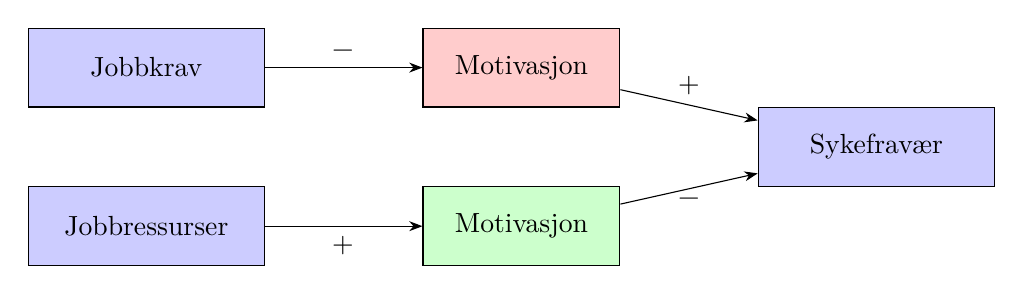
\begin{tikzpicture}[
      latent/.style={rectangle, draw, fill=blue!20, minimum width=3cm, minimum height=1cm},
      item/.style  ={rectangle, draw, fill=blue!10, font=\small},
      medi/.style  ={rectangle, draw, fill=green!20, minimum width=2.5cm, minimum height=1cm},
      medi2/.style ={rectangle, draw, fill=red!20,   minimum width=2.5cm, minimum height=1cm},
      moder/.style ={diamond,   draw, fill=yellow!20,aspect=2, minimum width=2.5cm, minimum height=1cm},
      >=Stealth,
      node distance=1cm and 2cm
    ]

    % Latente noder
    \node[latent]              (JK)  {Jobbkrav};
    \node[latent, below=of JK] (JR)  {Jobbressurser};

    % To separate motivasjons-noder
    \node[medi2, right=of JK] (M1) {Motivasjon};
    \node[medi,  right=of JR] (M2) {Motivasjon};

    % Piler fra latente til motivasjon med tegn
    \draw[->] (JK) -- node[midway, above] {$-$} (M1);
    \draw[->] (JR) -- node[midway, below] {$+$} (M2);

    % Sykefravær
    \node[latent, right=3cm of $(M1)!0.5!(M2)$] (SF) {Sykefravær};

    % Piler fra motivasjon til sykefravær med tegn
    \draw[->] (M1) -- node[midway, above] {$+$} (SF);
    \draw[->] (M2) -- node[midway, below] {$-$} (SF);

  \end{tikzpicture}
  \caption{JD–R-modellen}
  \label{fig:jdr_tikzz}
\end{figure}

Schaufeli \& Bakker (2004) testet i en SEM-analyse hvordan jobbkrav og
jobbressurser forklarer utbrenthet og jobbengasjement. Studien viste at
utbrenthet og jobbengasjement var negativt korrelert, og at jobbkravene
hadde en positiv effekt på utbrenthet, mens jobbressursene hadde en
signifikant \textbf{positiv} effekt på jobbengasjement. Dette kan
understøtte at høye krav skaper stress og fravær, mens ressurser fremmer
engasjement og opplevelse av mestring. Denne studien fokuserer på
hvordan utbrenthet har en medierende effekt på forholdet mellom jobbkrav
og helseproblemer, og engasjement medierer forholdet til jobbressurser
og intensjon om å slutte i arbeid. Studien deres inkluderte kun
respondenter fordelt på fire forskjellige arbeidsplasser og yrker, og vi
vil da videre fokusere på hvordan jobbkrav og jobbressurser påvirker
sykefravær gjennom motivasjon, og hvordan formue kan moderere disse
effektene for arbeidstakere i hele Norge.

\subsubsection{Formue i JD-R}\label{sec-formue-jdr}

Vi mener at økonomiske ressurser som formue, kan bidra til å forklare
sykefraværet og vil derfor inkludere formue som en direkte prediktor for
både motivasjon og sykefravær i vår modell.

Hobfoll (1989) definerer ressurser som noe som kan hjelpe individer med
å håndtere krav, og som kan fungere som en buffer mot stress
(Conservation of Resources (COR)-teori). Formue kan ses som en slik
økonomisk ressurs som gir en buffer som kan redusere sårbarheten for
både jobbrelatert og generelt stress. Personer med høy formue kan ha
større valgfrihet og tåle perioder med høy belastning eller økonomisk
usikkerhet bedre, uten at det nødvendigvis går like hardt utover helse
eller jobbmotivasjon. Motsatt vil personer med lav eller negativ formue
ofte være mer økonomisk avhengige av inntekten fra arbeid, og kan derfor
være mer sårbare for stressfaktorer.

Formue kan også ha betydning for fremtidsperspektiv og indre motivasjon.
Personer med lav formue kan oppleve mindre kontroll over egen
livssituasjon og lavere forventninger til fremtidig økonomisk trygghet,
noe som potensielt svekker arbeidsglede og motivasjon. Det er også mulig
at sammenhengen mellom formue og utfall som motivasjon eller sykefravær
ikke er lineær; effekten av økt formue kan være sterkere for de med lav
formue og avta med økende formuenivå (en bueformet effekt).

Selv om vår SEM-modell tester direkte lineære sammenhenger for formue,
er det teoretisk interessant å vurdere formue som en faktor som kan
påvirke hvordan individer opplever og håndterer jobbkrav og
jobbressurser. Denne mer komplekse rollen som moderator, hvor formue
endrer styrken på sammenhengen mellom arbeidsmiljøfaktorer og utfall, er
ikke direkte testet med interaksjonsledd i vår analyse, men tanken om at
formue kan dempe negative effekter av jobbkrav og forsterke positive
effekter av jobbressurser, er relevant. Üngüren et al. (2021) fant for
eksempel at økonomisk velvære\footnote{Økonomisk velvære kan defineres
  som en tilstand der en person fullt ut kan møte nåværende og løpende
  økonomiske forpliktelser, kan føle seg trygg på sin økonomiske
  fremtid, og er i stand til å ta valg som gjør det mulig å nyte livet.
  Financial Protection Bureau) (2015)} fungerte som en moderator som
reduserte den negative effekten av jobbusikkerhet på utbrenthet.

Ved å inkludere formue som en direkte prediktor i vår JD-R-inspirerte
modell, forsøker vi å fange noe av den direkte effekten av økonomisk
trygghet. I et samfunn med økende økonomisk ulikhet er det viktig å
forstå hvordan dette påvirker arbeidstakere og deres helse.

\subsection{Tidligere forskning}\label{tidligere-forskning}

Tidligere empirisk forskning har over tid vist positive forhold mellom
forskjellige Job Demands-Resources-faktorer og årsaker som kan føre til
sykefravær.

\subsubsection{Mikronivå: JD-R-studier i helse- og
omsorgssektoren}\label{mikronivuxe5-jd-r-studier-i-helse--og-omsorgssektoren}

Vander Elst et al. (2016) brukte en JD-R-modell hvor de utførte en
SEM-analyse på Belgisk hjemme-pleiepersonell. Jobbkrav og jobbressurser
ble modellert som prediktorer. Studien viste at jobbkravene var positivt
assosiert med utbrenthet, mens jobbressursene var positivt assosiert med
jobbengasjement. Denne studien viser også at JDR-mekanismer holder i
andre sammenhenger hvor arbeidstakere er under emosjonelt press og
skiftarbeid, noe som impliserer at JDR-modellen er robust på tvers av
sektorer og bransjer.

\subsubsection{Mikronivå:
formue-helse-koblinger}\label{mikronivuxe5-formue-helse-koblinger}

Jaeggi et al. (2021) undersøkte effekten av ulikhet i formue i et
småskala samfunn av innfødte i Tsimane i Bolivia med 871 observasjoner,
\(n = 871\). I studien testet de relativ husholdningrikdom og ulikhet i
formue mot forskjellige psykologiske variabler og helseutfall som
depresjon, BMI, blodtrykk og sykelighet.

Studien viste til en kobling mellom formueulikhet hvor de med lavere
formue hadde større sannsynlighet for å få høyere blodtrykk og
luftveissykdommer som kunne lede til dødsfall. De fant også at de med
høyere formue hadde lavere sannsynlighet for å få depresjon og høyere
BMI. Dette indikerer at ulikhet i formue kan moderere stress og
helserisiko på individnivå og vi antar da at dette kan være overførbart
til Norge, og at formue kan moderere effekten av jobbkrav og
jobbressurser på sykefravær.

\subsubsection{Mikronivå: JD-R-studier i
Norge}\label{mikronivuxe5-jd-r-studier-i-norge}

Langseth-Eide \& Vittersø (2021) bygger videre på tidligere forskning
ved JD-R-modellen. De argumenterer for at JD-R-modellen ved tidligere
forskning har hatt fokus på organisasjonsnivået, og at det er viktig å
se på hvordan JD-R-modellen kan brukes bedre på jobbressurser,
jobbengasjement og helserelaterte utfall. De gjorde en paneldata studie
på fast ansatte i Norge med to års tidsforsinkelse med 1533 ansatte
første tidsperiode, \(n =1533\) og 1503 ansatte, \(n = 1503\) neste
tidsperiode.

Over lengre tid fant de at jobbressurser hadde en positiv effekt på
jobbengasjement, og at jobbengasjement var negativt assosiert med
sykefravær. Dette impliserer at høyere jobbressurser kan føre til høyere
jobbengasjement, som igjen kan føre til lavere sykefravær i Norge, og
derfor vil vi bygge videre på denne studien ved å inkludere formue som
en moderator i JD-R-modellen.

\subsubsection{Makronivå: Ulikhet i
samfunnet}\label{makronivuxe5-ulikhet-i-samfunnet}

JD-R-modellen operer primært på individnivå, men en makroøkonomisk
studie om inntektsulikhet har vist at økonomisk ulikhet i en befolkning
korrelerer med høyere sykefravær og dårligere helse. Pickett \&
Wilkinson (2015) undersøkte sammenhengen mellom inntektsulikhet og helse
i 34 OECD-land, og fant at høyere inntektsulikhet var assosiert med
høyere sykefravær og dårligere helseutfall. Studien viste også at
inntektsulikhet hadde en negativ effekt på livskvalitet og trivsel, og
at dette kunne føre til økt sykefravær. Det kan antas at inntektsulikhet
forsterker psykososialt stress ved lav formue, derfor vil vi undersøke
hvordan formue påvirker sykefravær i Norge, og hvordan formue kan
moderere effekten av jobbkrav og jobbressurser på sykefravær.

Mekanismene som følger på mikronivå er da:

\[
\text{Høyere jobbkrav} \rightarrow \text{Økt utbrenthet} \rightarrow \text{Høyere sykefravær}
\]

\[
\text{Høyere jobbressurser} \rightarrow \text{Økt jobbengasjement} \rightarrow \text{Lavere sykefravær}
\]

Hvor formue fungerer som en moderator ved å påvirke stress til individer
før jobbkravene utløser negative effekter på helse.

På makronivå vil samfunnsmessig ulikhet forme de jobbkrav og ressurser
som virksomheter og arbeidstakere får, og dermed styrke JDR-mekanismer,
også på tvers av sektorer og bransjer. Dermed får vi et teoretisk og
empirisk grunnlag for vår undersøkelse av at:

\[
\text{Formue} \rightarrow \text{Jobbkrav og jobbressurser} \rightarrow \text{Sykefravær i Norge}
\]

\subsection{Modelloppsett}\label{modelloppsett}

Modellen vi blir å bruke blir da som følger:

\begin{figure}
  \centering
  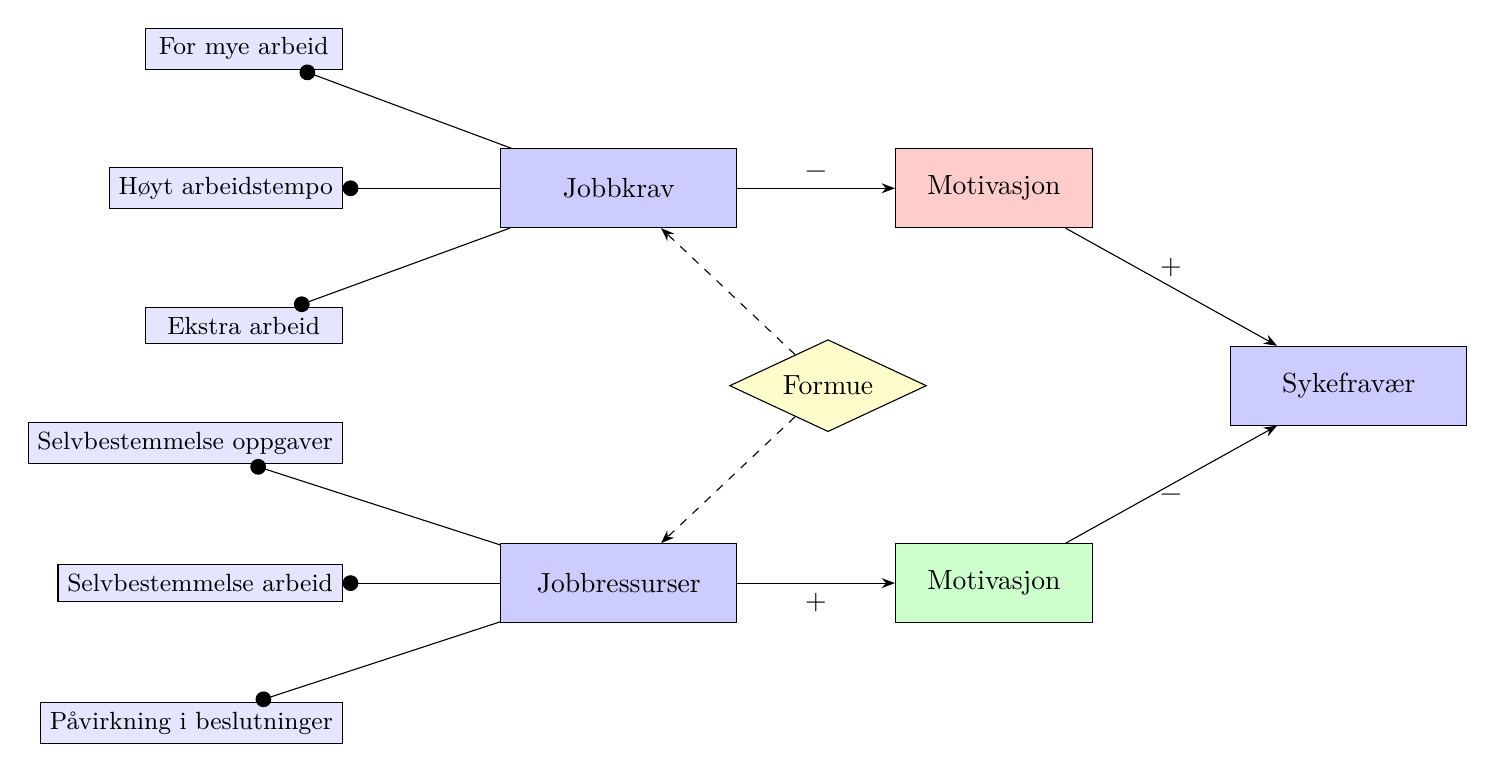
\begin{tikzpicture}[
      latent/.style={rectangle, draw, fill=blue!20, minimum width=3cm, minimum height=1cm},
      item/.style  ={rectangle, draw, fill=blue!10, font=\small, minimum width=2.5cm},
      medi/.style  ={rectangle, draw, fill=green!20, minimum width=2.5cm, minimum height=1cm},
      medi2/.style ={rectangle, draw, fill=red!20,   minimum width=2.5cm, minimum height=1cm},
      moder/.style ={diamond,   draw, fill=yellow!20,aspect=2, minimum width=2.5cm, minimum height=1cm},
      >=Stealth,
      node distance=1cm and 2cm
    ]

    % Latente noder
    \node[latent]              (JK)  {Jobbkrav};
    \node[latent, below=of JK, yshift=-3cm] (JR) {Jobbressurser};

    % Indikator-noder for Jobbkrav
    \node[item, above left=of JK]      (v1) {For mye arbeid};
    \node[item, left=of JK]            (v2) {Høyt arbeidstempo};
    \node[item, below left=of JK]      (v5) {Ekstra arbeid};
    \draw[-{Circle[length=2mm]}] (JK) -- (v1);
    \draw[-{Circle[length=2mm]}] (JK) -- (v2);
    \draw[-{Circle[length=2mm]}] (JK) -- (v5);

    % Indikator-noder for Jobbressurser
    \node[item, above left=of JR]            (v3) {Selvbestemmelse oppgaver};
    \node[item, left=of JR]      (v4) {Selvbestemmelse arbeid};
    \node[item, below left=of JR, yshift=0cm] (v6) {Påvirkning i beslutninger};
    \draw[-{Circle[length=2mm]}] (JR) -- (v3);
    \draw[-{Circle[length=2mm]}] (JR) -- (v4);
    \draw[-{Circle[length=2mm]}] (JR) -- (v6);

    % Moderator-node plassert midt over
    \node[moder, right=1.4cm of $(JK)!0.5!(JR)$] (FN) {Formue};
    \draw[->, dashed] (FN) -- (JK);
    \draw[->, dashed] (FN) -- (JR);

    % To separate motivasjons-noder
    \node[medi2, right=of JK] (M1) {Motivasjon};
    \node[medi,  right=of JR] (M2) {Motivasjon};

    % Piler fra latente til motivasjon med tegn
    \draw[->] (JK) -- node[midway, above] {$-$} (M1);
    \draw[->] (JR) -- node[midway, below] {$+$} (M2);

    % Sykefravær
    \node[latent, right=3cm of $(M1)!0.5!(M2)$] (SF) {Sykefravær};

    % Piler fra motivasjon til sykefravær med tegn
    \draw[->] (M1) -- node[midway, above] {$+$} (SF);
    \draw[->] (M2) -- node[midway, below] {$-$} (SF);

  \end{tikzpicture}
  \caption{Utvidet JD–R-modell med formue som moderator, indikatorer og motivasjonsløp.}
  \label{fig:jdr_tikz}
\end{figure}

I modellen vår (\autoref{fig:jdr_tikz}) har vi inkludert formue som en
moderator som påvirker både jobbkrav og jobbressurser. Dette betyr at
formue kan endre hvordan jobbkrav og jobbressurser påvirker
sykefraværet. Vi har også separate motivasjonsløp for jobbkrav og
jobbressurser, som gjør at vi kan se hvordan motivasjon påvirkes av
begge disse faktorene. Vi antar at formuen blir å fungere som en
stress-avlastning eller buffer mot jobbkravene og forsterke effekten av
jobbressurser, og fungere som en psykologisk trygghet. Dette kan føre
til at personer med høyere formue opplever lavere sykefravær, mens de
med lavere formue kan oppleve høyere sykefravær på grunn av økt stress
og lavere tilgang til ressurser.

\subsubsection{Hypoteseliste}\label{hypoteseliste}

Med dette rammeverket formulerer vi følgende hypoteser:

\textbf{H1:} Høyere jobbkrav gir høyere sykefravær (Direkte effekt
\(JK \rightarrow SF\))

\textbf{H2:} Høyere jobbressurser gir lavere sykefravær (Direkte effekt
\(JR \rightarrow SF\))

\textbf{H3:} Høyere formuenivå gir lavere sykefravær (Primært via økt
motivasjon \(FN \rightarrow M \rightarrow SF\) men også direkte effekt
\(FN \rightarrow SF\))

\textbf{H4:} Jobbressurser og formue øker motivasjon (Direkte effekter
\(JR \rightarrow M\) og \(FN \rightarrow M\))

For en grundig gjennomgang av hypotesene og hvordan de er relatert til
JD-R-modellen, se kapittel \ref{sec-hypot}.

\section{Data}\label{data}

I dette kapitlet går vi gjennom datagrunnlaget for oppgaven. Vi vil
først forklare hvordan dataene er fremskaffet for å så forklare
variablene. Vi vil også gi en innledende oversikt over dataene,
inkludert deskriptiv statistikk for alle variablene i analysen.

I problemstillingen \emph{forklarer nivået på formue sykefraværet i
Norge?} så velger vi å bruke en Structural Equation Model fordi denne
kan bedre vise oss hvordan formue påvirker sykefraværet, inkludert
eventuelle indirekte sammenhenger via motivasjon, mellom variablene vi
velger å bruke. Dette gjør analysen mer kompleks, men vi kan bedre peke
på hvilke effekter som er positive eller negative på selve sykefraværet.

Dataen vi bruker er hentet fra Statistisk sentralbyrå (SSB) sin
\href{https://www.ssb.no/arbeid-og-lonn/arbeidsmiljo-sykefravaer-og-arbeidskonflikter/artikler/levekarsundersokelsen-om-arbeidsmiljo-2022}{levekårsundersøkelse
om arbeidsmiljø}, som ble gjennomført i 2022. Vedlagt følger et bilde av
kodeboken:


\includegraphics{dokumentobjekter/bilder/codebook.png}

Statistisk sentralbyrå har gjennomført levekårsundersøkelser siden 1973.
Levekårsundersøkelsen kartlegger arbeidsmiljøforhold blant sysselsatte i
Norge, og tar opp temaer som forhold på arbeidsplassen, fysisk,
ergonomisk og psykososialt arbeidsmiljø, yrkesrelaterte helseplager og
sykefravær og krav og muligheter for selvbestemmelse på jobb.

\subsection{Datakilde og utvalg}\label{datakilde-og-utvalg}

Undersøkelsen er basert på et landsrepresentativt utvalg på 35 345
sysselsatte personer i alderen 18-66 til undersøkelsen i 2022. Utvalget
er tilfeldig trukket fra folkeregisteret, og dataene er samlet inn
gjennom telefonintervjuer og selvadministrert webskjema fra august 2022
til april 2023.

Den totale svarprosenten for undersøkelsen var på 51 prosent, og dataene
er vektet for å være representativt for den norske befolkningen i
alderen 18-66 for å korrigere for noen av skjevhetene i forbindelse med
frafall.

\subsection{Variabler}\label{variabler}

Vi kommer til å bruke flere variabler fra levekårsundersøkelsen for å
analysere sammenhengen mellom formue og sykefravær. Vi vil bruke både
avhengige og uavhengige variabler, latente variabler, samt
kontrollvariabler for å kontrollere for andre faktorer som kan påvirke
sykefraværet.

\subsubsection{Avhengig og uavhengig
hovedvariabel}\label{avhengig-og-uavhengig-hovedvariabel}

Sykefravær:

Datasettet inneholder en ferdig variabel for sykefraværsprosent
(sfpros\_uten\_feriekorr\_2022, sfpros\_uten\_feriekorr\_2023), men vi
velger å beregne denne selv siden de med 0 fravær står som NA, også for
å kunne ta høyde for avtalt arbeidstid.

Vi benytter variablene sfdagsvj\_2022 (sykefraværsdagsverk) og
mdagsv\_2022 (avtalte dagsverk) fra Levekårsundersøkelsen.
Sykefraværsraten (\(SF_i\)) for individ \(i\) beregnes som:

\[
SF_i = 
\begin{cases}
0, & \text{hvis } \mathrm{mdagsv\_2022}_i > 0 \text{ og } \mathrm{sfdagsvj\_2022}_i = 0 \\
\frac{ \mathrm{sfdagsvj\_2022}_i }{ \mathrm{mdagsv\_2022}_i }, & \text{hvis } \mathrm{mdagsv\_2022}_i > 0 \text{ og } \mathrm{sfdagsvj\_2022}_i > 0 \\
\text{NA}, & \text{hvis } \mathrm{mdagsv\_2022}_i \leq 0
\end{cases}
\]

Dette gjør at individer med avtalte dagsverk, men uten legemeldt
sykefraværsdager, får verdien 0 i stedet for NA slik det gjøres i den
ferdigberegnede variabelen sfpros\_uten\_feriekorr\_2022.

Vi har fjernet alle som har over 14 dager sammenhengende sykefravær, for
å unngå å inkludere langtidssykemeldte som kan ha andre årsaker til
fravær enn de vi ønsker å undersøke. Dette gjør at vi får et mer
representativt bilde av korttidsfravær og dets sammenheng med formue.

Formue:

Bruttofinanskapital i alt vil være vår hoveduavhengige variabel, og vi
vil bruke bruttofinanskapital i alt som mål på formue. Denne variabelen
inneholder verdien av alle finansielle eiendeler som respondenten eier,
inkludert kontanter, aksjer, obligasjoner og andre investeringer og har
en maks verdi på 2 500 000.

Formuefordelingen er veldig høyreskjev med mange individer med lav
formue og få med svært høy formue. Denne skjevheten med mange
observasjoner i den nedre enden av formuefordelingen og få i den øvre
enden, kan skape problemer for analysen vår. Gjennomsnitt vil være
sterkt påvirket av de få ytre ekstreme verdiene og vi kan se at
variansen ikke er konstant.

Vi kan ikke forvente lineære sammenhenger over hele skalaen så for å
håndtere denne skjevheten og representere formue på en skala som bedre
viser den relative formuen til individer, så transformerer vi
formuevariabelen. Vi bruker en invertert kumulativ fordeling\footnote{Invertert
  kumulativ fordeling er en metode for å transformere en variabel slik
  at den følger en normalfordeling, og brukes ofte for å håndtere
  skjevheter i data.} (ved bruk av qnorm i R) for å normalisere
formuefordelingen. Vi gjør dette med samme begrunnelse som Gugushvili \&
Wiborg (2025) hvor det gjøres for å kunne sammenligne den relative
formuen til individer i stedet for den absolutte formuen.

Resultatet er en variabel der hver individets formuesverdi er erstattet
med en Z-skåre som reflekterer deres relative posisjon i
formuefordelingen, men på en skala som er tilnærmet normalfordelt, som
vist i \autoref{fig:histogram_formue_fordeling}. En verdi på 0 på
Formue\_qnorm indikerer en formue nær medianen (eller gjennomsnittet,
siden fordelingen nå er relativt symmetrisk). En verdi på -1 indikerer
en formue omtrent ett standardavvik under medianen, og +1 ett
standardavvik over.

Denne metoden rangerer alle de observerte formueverdiene for å
konvertere dem til Z-skårer fra en standard normalfordeling. Dette gjør
at variabelen er mindre sensitiv for ekstreme verdier, og at vi kan
bruke formue som en kontinuerlig variabel i analysen.

Vi definerer lav formue som de mer enn et standardavvik under
gjennomsnittet, middels formue som de innenfor ett standardavik, og høy
formue som de mer enn ett standardavvik over gjennomsnittet.

En av våre hypoteser er at formue påvirker individets sensitivitet for
inntektsendringer. Altså individets konsumnnivå eller etterspurt fritid
endrer seg ulikt basert på om de har mye formue eller ikke. Dette kan
være fordi individet har mer buffer til å tåle endringer i inntekt, og
dermed kan individet være mer villig til å ta seg fri fra jobb. Motsatt
vil individer med lav formue være mer sårbare for inntektsendringer, og
kan derfor være mindre tilbøyelige til å være borte fra jobb, selv ved
sykdom, for å opprettholde sin inntekt. Dette kan bety at de med høyere
formue har bedre forutsetninger for å opprettholde god helse som ved en
mindre belastende jobbsituasjon, noe som kan føre til lavere sykefravær,
mens de med lavere formue opplever mer stress knyttet til økonomi, som
kan gi høyere sykefravær.

\subsubsection{Latente variabler}\label{latente-variabler}

Jobbkrav:

Jobbkrav er en latent variabel som vi måler med tre indikatorer: For mye
arbeid (QPS15\_ny), Høyt arbeidstempo (QPS14\_ny) og Ekstra arbeid
(Sp47f). Disse indikatorene er basert på spørsmål i
Levekårsundersøkelsen som måler hvor mye arbeid respondenten opplever at
de har, hvor høyt tempo de opplever på jobben, og om de ofte må gjøre
ekstra arbeid utenom det som er avtalt. Disse indikatorene vil gi oss en
indikasjon på hvor høye jobbkravene er for individet.

Jobbressurser:

Jobbressurser er en latent variabel som vi måler med fire indikatorer:
Grad av selvbestemmelse over oppgaver (Sp56a2), Grad av selvbestemmelse
over arbeid som skal gjøres (Sp56b2), Grad av påvirkning på beslutninger
i arbeidet (QPS53) og til hvilken grad man kan bestemme eget
arbeidstempo (QPS47). Disse indikatorene er basert på spørsmål i
Levekårsundersøkelsen som måler hvor mye støtte og ressurser
respondenten opplever at de har på jobben, og hvor mye kontroll de har
over eget arbeid. Disse indikatorene vil gi oss en indikasjon på hvor
gode jobbressursene er for individet.

\subsubsection{Kontrollvariabler}\label{kontrollvariabler}

Alder:

Alder til respondenten ved utgangen av 2022. Denne kontrollvariabelen
gjør vi ordinal ettersom vi fordeler alderen til respondenten i
aldersgrupper. Vi vil bruke aldersgruppene 18-29, 30-54 og 55-66 år. Da
kan vi påpeke hvis det er forskjeller i sykefravær mellom de
forskjellige aldersgruppene fra unge til eldre personer.

Kjønn:

Kjønn til respondenten. Denne kontrollvariabelen er en dummyvariabel,
hvor 0 er kvinne og referansekategorien 1 er menn. Da vil vi i analysen
direkte se effekten av å være kvinne på sykefraværet.

Utdanning:

Utdanningsnivået til respondenten er en ordinal variabel, og vi vil
bruke utdanningsgruppene grunnskole eller mindre, videregående skole,
Universitet/Høgskole og forskernivå. Denne variabelen inkluderes for å
justere for mulige utdanningsrelaterte forskjeller i sykefravær.

Motivasjon:

For variabelen motivasjon bruker vi selvrapportert motivasjon på jobb
(M) som en ordinal variabel, og vi vil bruke denne variabelen for å
kontrollere for eventuelle forskjeller i sykefraværet basert på hvor
motivert respondenten er på jobben sin. Variabelen er basert på en skala
med 5 nivåer (1=svært sjelden/aldri motivert til 5=veldig ofte
motivert).

Barn:

Har barn under 5 år i husholdningen som er en kategorisk variabel. Vi
vil bruke denne variabelen for å kontrollere for eventuelle forskjeller
i sykefraværet basert på om respondenten har barn under 5 år.

Stillingsprosent (\(SP_i\)):

Antall timer en person arbeider er en sentral faktor som kan påvirke
både eksponering for jobbkrav og jobbressurser og forekomsten av
sykefravær. Studien til Langseth-Eide (2019) om ``workaholism'' og
jobbengasjement innenfor JD-R-modellen, viser at et høyt timeantall på
jobb ikke er et ensartet fenomen. Både ansatte som er ``workaholics''
(med potensielt negative helsekonsekvenser) og de som er høyt
jobbengasjerte (ofte med positive helseeffekter) kan rapportere å jobbe
mer enn forventet. Dette indikerer at årsakene til, og konsekvensene av,
mange arbeidstimer kan variere betydelig.

For å ta høyde for denne kompleksiteten og kontrollere for variasjon i
arbeidsomfang, inkluderer vi respondentens avtalte stillingsprosent
(arb\_stillingspst) som en kontrollvariabel. Denne variabelen
reflekterer den formelle arbeidsmengden. Ved å inkludere
stillingsprosent (\(SP_i\)) i modellen, kan vi forsøke å se effekten for
en ulik ``eksponeringstid''.

\subsection{Deskriptiv statistikk}\label{deskriptiv-statistikk}

I dette avsnittet vil vi gi en oversikt over deskriptiv statistikk for
alle variablene i analysen. Vi vil presentere gjennomsnitt,
standardavvik og minimums- og maksimumsverdier for alle variablene, samt
korrelasjonsmatrisen for de uavhengige variablene.

I \autoref{tab:deskriptiv} presenteres deskriptiv statistikk for alle
variablene i analysen. Vi ser at sykefraværet i 2022 har et gjennomsnitt
på 1.70 prosent (0.00170), med en minsteverdi på 0 prosent og
maksimalverdi på 48.08 prosent. Alder ligger på et gjennomsnitt på 43.33
år, med en minsteverdi på 18 år og maksimalverdi på 66, som stemmer med
alderen til respondentene i datasettet. Utdanningsnivået har et
gjennomsnitt på 4.65, som tilsvarer videregående skole, med en
minimumsverdi på 2 (grunnskole eller mindre) og en maksimumsverdi på 8
(doktorgrad).

Av de opprinnelig 17971 inviterte respondentene i datasettet så
fullførte 6 103 svarene til alle de relevante variablene etter at vi
fjernet de som var langtidssykemeldt over 2 uker. Den endelige andelen
av de inviterte blir da \(\frac{6103}{17971} = 33.9\%\). Dette kan føre
til skjevheter i dataene, og kan bli en svakhet ved analysen når vi
tolker resultatene. Siden det er vanskelig for oss å vite om det er
systematiske forskjeller mellom de som svarte og de som ikke svarte, så
kan vi ikke si noe sikkert om hvor representativt utvalget er for den
norske befolkningen.

\begin{table}[ht]
\centering
\begin{tabular}{lrrrrrrr}
\toprule
Variabel                               & Min    & 1.\,Q  & Median & Mean   & 3.\,Q  & Max    & N    \\
\midrule
Sykefravær 2022                        & 0.0000 & 0.0000 & 0.0000 & 0.0170 & 0.0193 & 0.4808 & 6103 \\
Alder                                  & 18     & 33     & 45     & 43.33  & 54     & 66     & 6103 \\
Utdanning                              & 2      & 4      & 4      & 4.65   & 6      & 8      & 6103 \\
Tilfredshet                            & 1      & 4      & 4      & 4.19   & 5      & 5      & 6103 \\
Motivasjon                             & 1      & 4      & 4      & 4.03   & 5      & 5      & 6103 \\
Barn                                   & 0      & 0      & 0      & 0.14   & 0      & 1      & 6103 \\
Selvbestemmelse (oppgaver)             & 1      & 2      & 3      & 3.03   & 4      & 5      & 6103 \\
Selvbestemmelse (arbeidsinnhold)       & 1      & 3      & 4      & 3.73   & 4      & 5      & 6103 \\
Grad arbeidstempo                      & 1      & 3      & 4      & 3.37   & 4      & 5      & 6103 \\
Påvirkningsgrad                        & 1      & 3      & 3      & 3.47   & 4      & 5      & 6103 \\
For mye arbeid                         & 1      & 3      & 4      & 3.95   & 5      & 5      & 6103 \\
Høyt arbeidstempo                      & 1      & 4      & 4      & 4.13   & 5      & 5      & 6103 \\
Ekstra arbeid                          & 1      & 1      & 2      & 2.63   & 4      & 5      & 6103 \\
Stillingsprosent                       & 0      & 100    & 100    & 90.66  & 100    & 120    & 6103 \\
\bottomrule
\end{tabular}
\caption{Deskriptiv statistikk for hovedvariabler (N = 6103)}
\label{tab:deskriptiv}
\end{table}

I \autoref{tab:deskr_formue} ser vi at sykefraværet i 2022 har et
gjennomsnitt på 2 prosent (0.02) for de med lav formue, 2 prosent (0.02)
for de med middels formue og 1 prosent (0.01) for de med høy formue.
Dette antyder at de med høyere formue har litt lavere sykefravær, selv
om forskjellene er relativt små.

Alderen øker noe med formuegruppe: gjennomsnittsalderen er 40.44 år i
lav formue, 42.43 år i middels formue og 49.96 år i høy formue. Når
motivasjon måles på skalaen 1--5, er gjennomsnittsskårene 3.98 i lav
formue, 4.02 i middels formue og 4.15 i høy formue.

Forskjellene i motivasjon er små, men systematisk: personer med høy
formue rapporterer noe høyere motivasjon enn de med lav formue,
tilfredshet følger også omtrent samme mønster (4.14 mot 4.17 og
4.29).Samtidig ser vi at de med høyest formue også har den høyeste
gjennomsnittsalderen, noe som indikerer en kobling mellom alder og
formue (eldre personer har gjerne opparbeidet mer formue).

\begin{table}[H]
\centering
\begin{tabular}{lcccccc}
\toprule
                        & \multicolumn{2}{c}{Lav formue (n = 883)} 
                        & \multicolumn{2}{c}{Middels formue (n = 4255)} 
                        & \multicolumn{2}{c}{Høy formue (n = 965)}         \\
\cmidrule(r){2-3}\cmidrule(lr){4-5}\cmidrule(l){6-7}
Variabel                & M      & SD     & M       & SD     & M      & SD    \\
\midrule
Alder                   & 40.44  & 12.61  & 42.43   & 12.41  & 49.96  & 10.24 \\
Motivasjon              &  3.98  &  0.98  &  4.02   &  0.90  &  4.15  &  0.83 \\
Tilfredshet             &  4.14  &  0.88  &  4.17   &  0.85  &  4.29  &  0.76 \\
Sykefravær 2022         &  0.02  &  0.05  &  0.02   &  0.04  &  0.01  &  0.03 \\
\bottomrule
\end{tabular}
\caption{Deskriptiv statistikk etter formuegruppe}
\label{tab:deskr_formue}
\end{table}

I \autoref{tab:deskr_kjonn} presenteres deskriptiv statistikk for
sykefravær etter kjønn. Vi ser at sykefraværet i 2022 har et
gjennomsnitt på 1 prosent for menn og 2 prosent for kvinner, kvinner har
da dobbelt så høyt sykefravær enn menn. Dette kan skyldes at kvinner i
større grad enn menn jobber i yrker med høyere sykefravær, eller at
kvinner er mer tilbøyelige til å rapportere sykefravær enn menn. Det kan
også være andre faktorer som påvirker sykefraværet, som for eksempel
alder, utdanning og arbeidsforhold. Vi ser også at vi har en bra
fordeling av kvinner og menn i utvalget, der 47.9 prosent av
respondentene er kvinner og 52.1 prosent er menn.

\begin{table}[ht]
\centering
\begin{tabular}{lrrrr}
\toprule
Kjønn   & N   & \%   & Gj.snitt sykefravær & SD    \\
\midrule
Mann    & 3177 & 52.1 & 1\% (0.01)               & 4 (0.04) \\
Kvinne  & 2926 & 47.9 & 2\% (0.02)               & 4 (0.04) \\
\bottomrule
\end{tabular}
\caption{Deskriptiv statistikk for sykefravær etter kjønn (N = 6103)}
\label{tab:deskr_kjonn}
\end{table}

I \autoref{tab:deskr_utdanning} presenteres deskriptiv statistikk for
sykefravær etter utdanningsnivå. Vi ser at sykefraværet i 2022 har et
gjennomsnitt på 2 prosent for de med grunnskole eller mindre, 2 prosent
for de med videregående skole og 1 prosent for de med
universitet/høgskole. Dette tyder på at sykefraværet er høyere for de
med lavere utdanning, og at det kan være en liten sammenheng mellom
utdanningsnivå og sykefravær.

\begin{table}[ht]
\centering
\begin{tabular}{lrrrr}
\toprule
Utdanningsnivå                & N    & \%   & Gj.snitt sykefravær & SD   \\
\midrule
Grunnskole eller mindre       & 816 & 13.3 & 2\% (0.02)                    & 4 (0.04)   \\
Videregående                   & 2941 & 48.2 & 2\% (0.02)                  & 4 (0.04)   \\
Universitet/Høgskole           & 2346 & 38.5 & 1\% (0.01)                   & 4 (0.04)  \\
\bottomrule
\end{tabular}
\caption{Deskriptiv statistikk for sykefravær i 2022 etter utdanningsnivå (N = 6103).}
\label{tab:deskr_utdanning}
\end{table}

\clearpage

\subsubsection{Figurer}\label{figurer}

I \autoref{fig:histogram_sykefravar} presenteres histogram og
tetthetskurve for sykefraværet i 2022. Vi ser at sykefraværet er veldig
høyreskjevt, med en høyere andel av respondentene som har lavt
sykefravær enn de som har høyt sykefravær både på menn og kvinner. Vi
vet fra \autoref{tab:deskr_kjonn} at gjennomsnittet er på 3 prosent for
menn mens det er på 6 prosent for kvinner, noe som gjenspeiles i grafen.
Det er vanskelig å se, men det er også noen uteliggere hvor flere
respondenter har mer enn 40 prosent sykefravær på både menn og kvinner,
noe som fører til halen som strekker seg mot høyre i histogrammet.

\begin{figure}[H]
\caption{Sykefravær i 2022}
\label{fig:histogram_sykefravar}
\centering
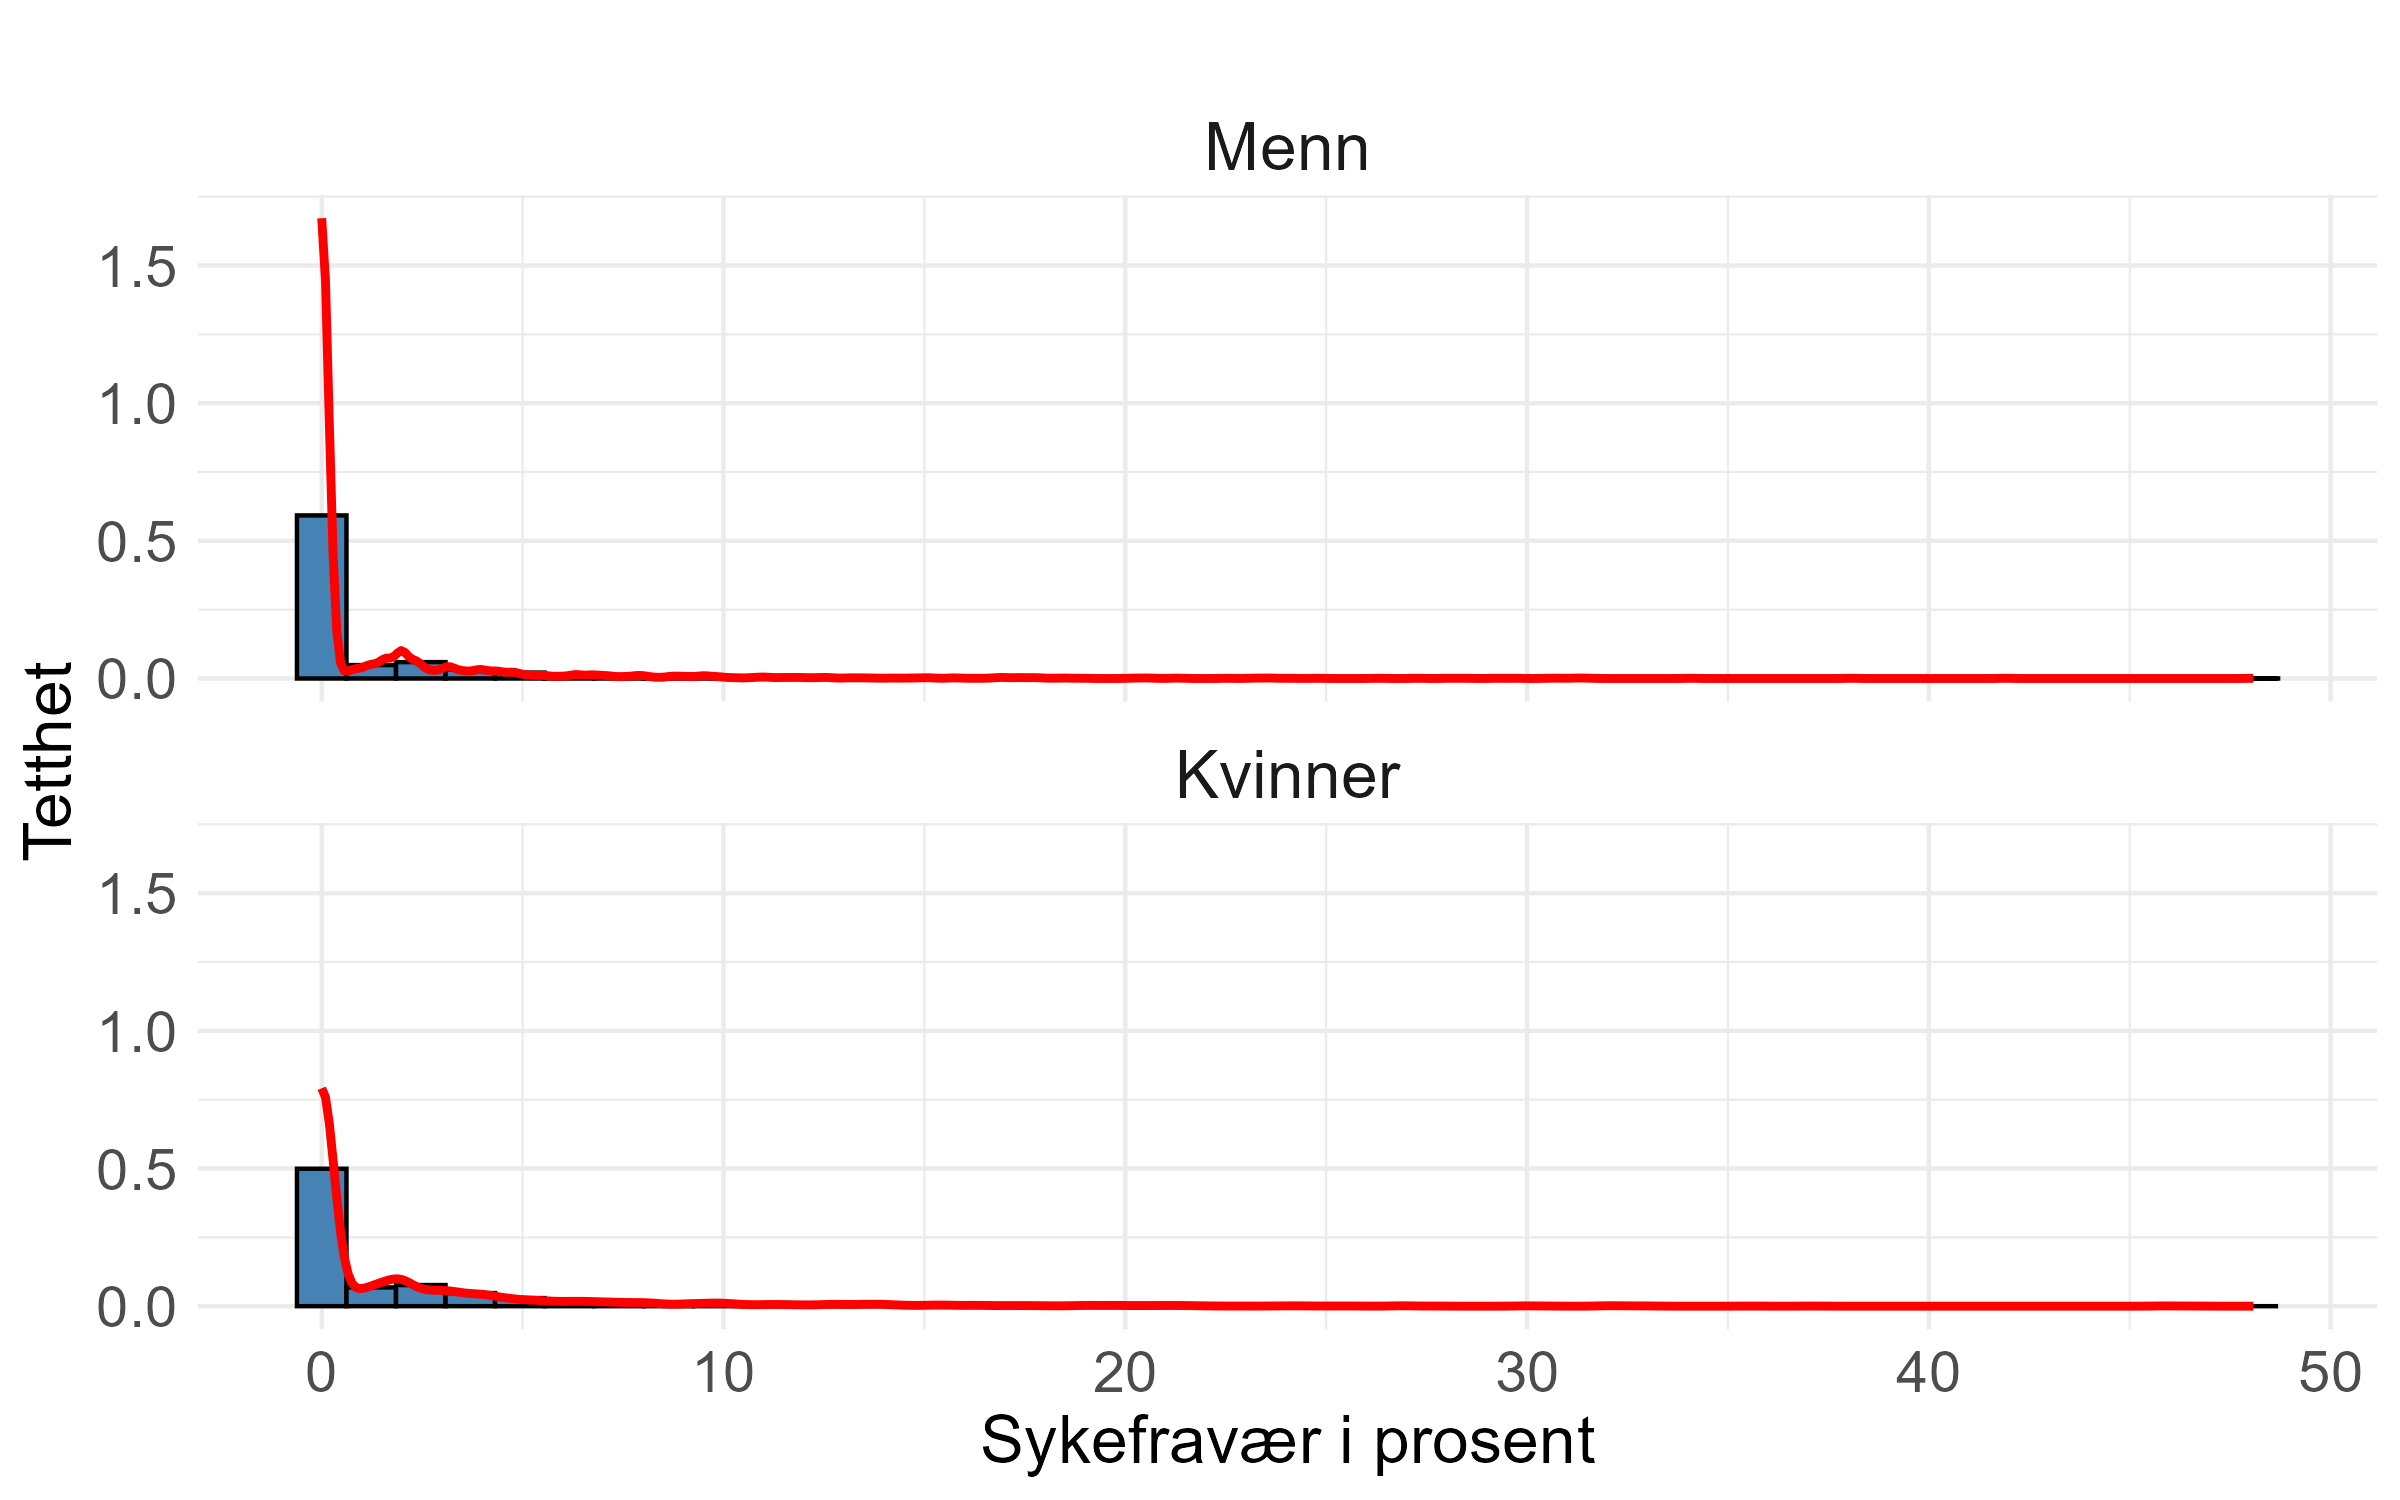
\includegraphics[width=0.8\textwidth]{dokumentobjekter/figurer/fig_sykefrav.png}
\end{figure}

I 2022 var det \(n=4081\) som hadde 0\% sykefravær, dette gjør at vår
fordeling er tydelig høyreskjev. I
\autoref{fig:histogram_sykefravar_log} er sykefraværet logtransformert
med +0.01, noe som fører til å glatte ut fordelingen og gjøre den mer
normalfordelt. Dette er en vanlig teknikk for å håndtere høyreskjeve
fordelinger, og det gjør at vi kan gjøre analysen vår mer robust mot
skjevheter. Men selv om vi har logtransformert sykefraværet, så er det
fortsatt mange som har lavt sykefravær, noe som kan påvirke resultatene
våre.

\vspace{-0.5cm}
\begin{figure}[H]
\caption{Sykefravær i 2022 logtransformert med +0.01}
\label{fig:histogram_sykefravar_log}
\centering
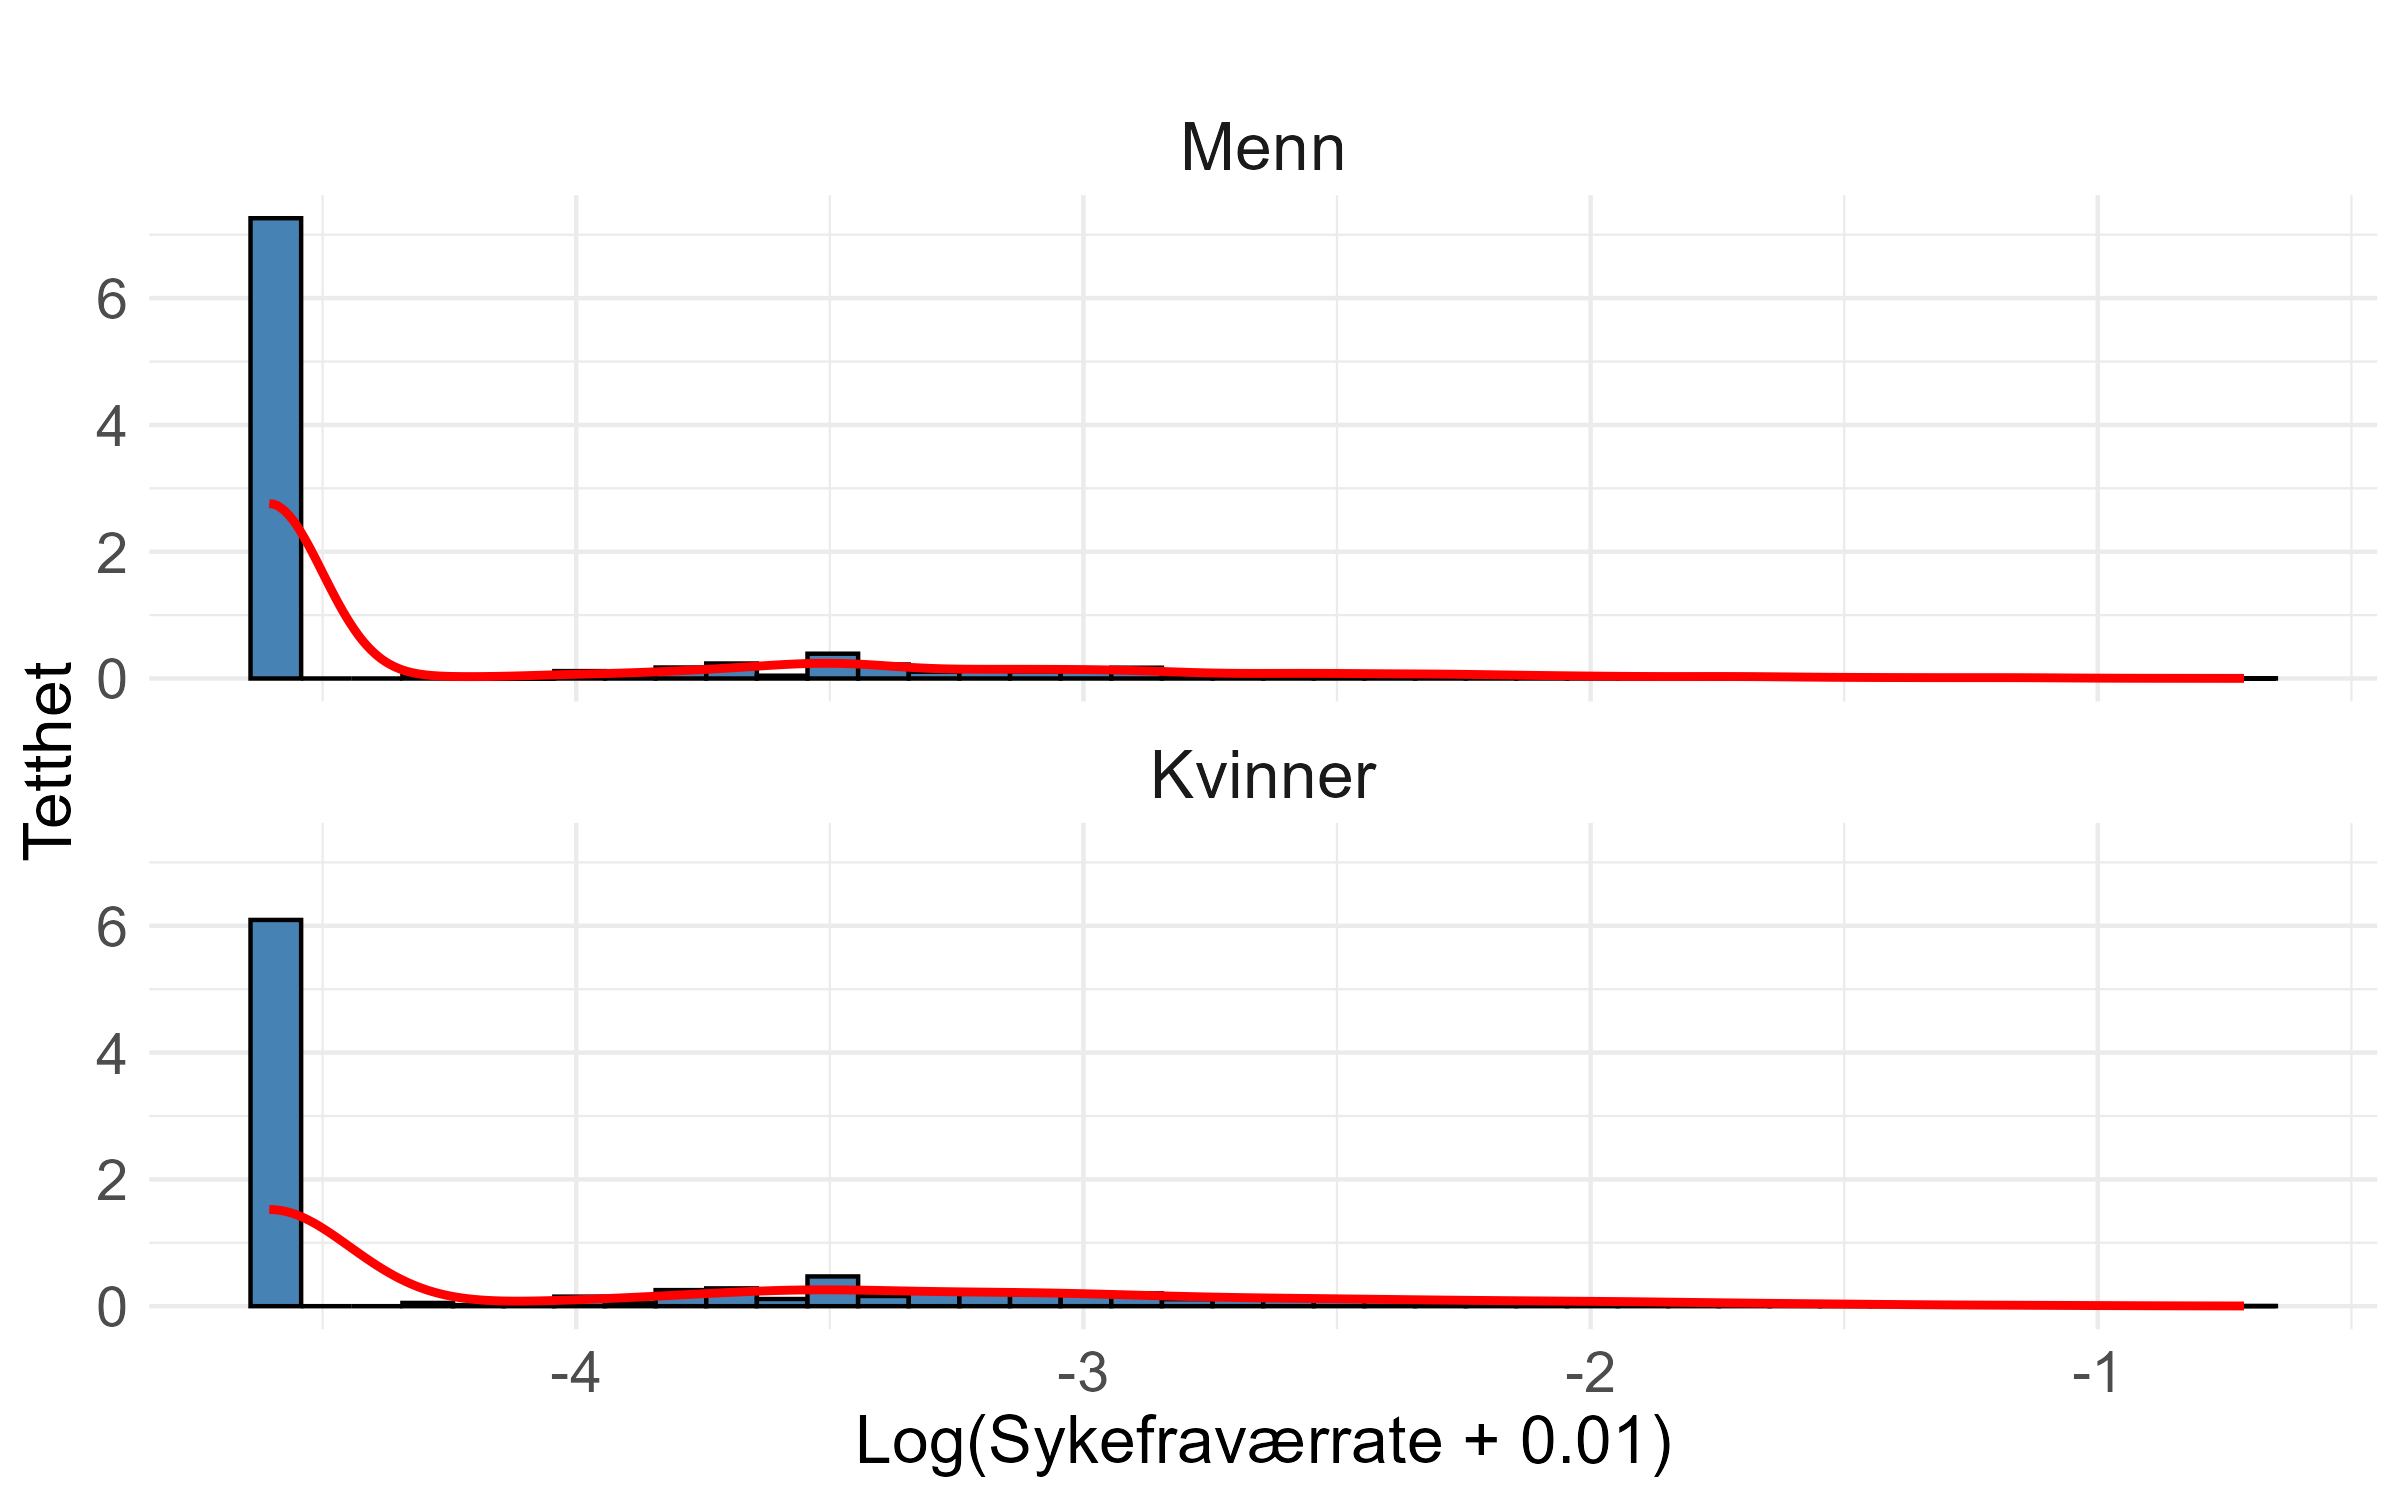
\includegraphics[width=0.8\textwidth]{dokumentobjekter/figurer/fig_sykefrav_log.png}
\end{figure}

Når vi ser på aldersfordelingen i \autoref{fig:histogram} så ser vi at
den er jevn og symmetrisk fordelt blant respondentene. Som nevnt
tidligere så er spennet på alderene til respondentene i undersøkelsen
mellom 18 til 66 år. Medianalderen kan man se i den blå stiplede linjen
som er på 44 år for menn og 45 år for kvinner.

\begin{figure}[H]
\caption{Histogram og tetthetskurve for alder}
\label{fig:histogram}
\centering
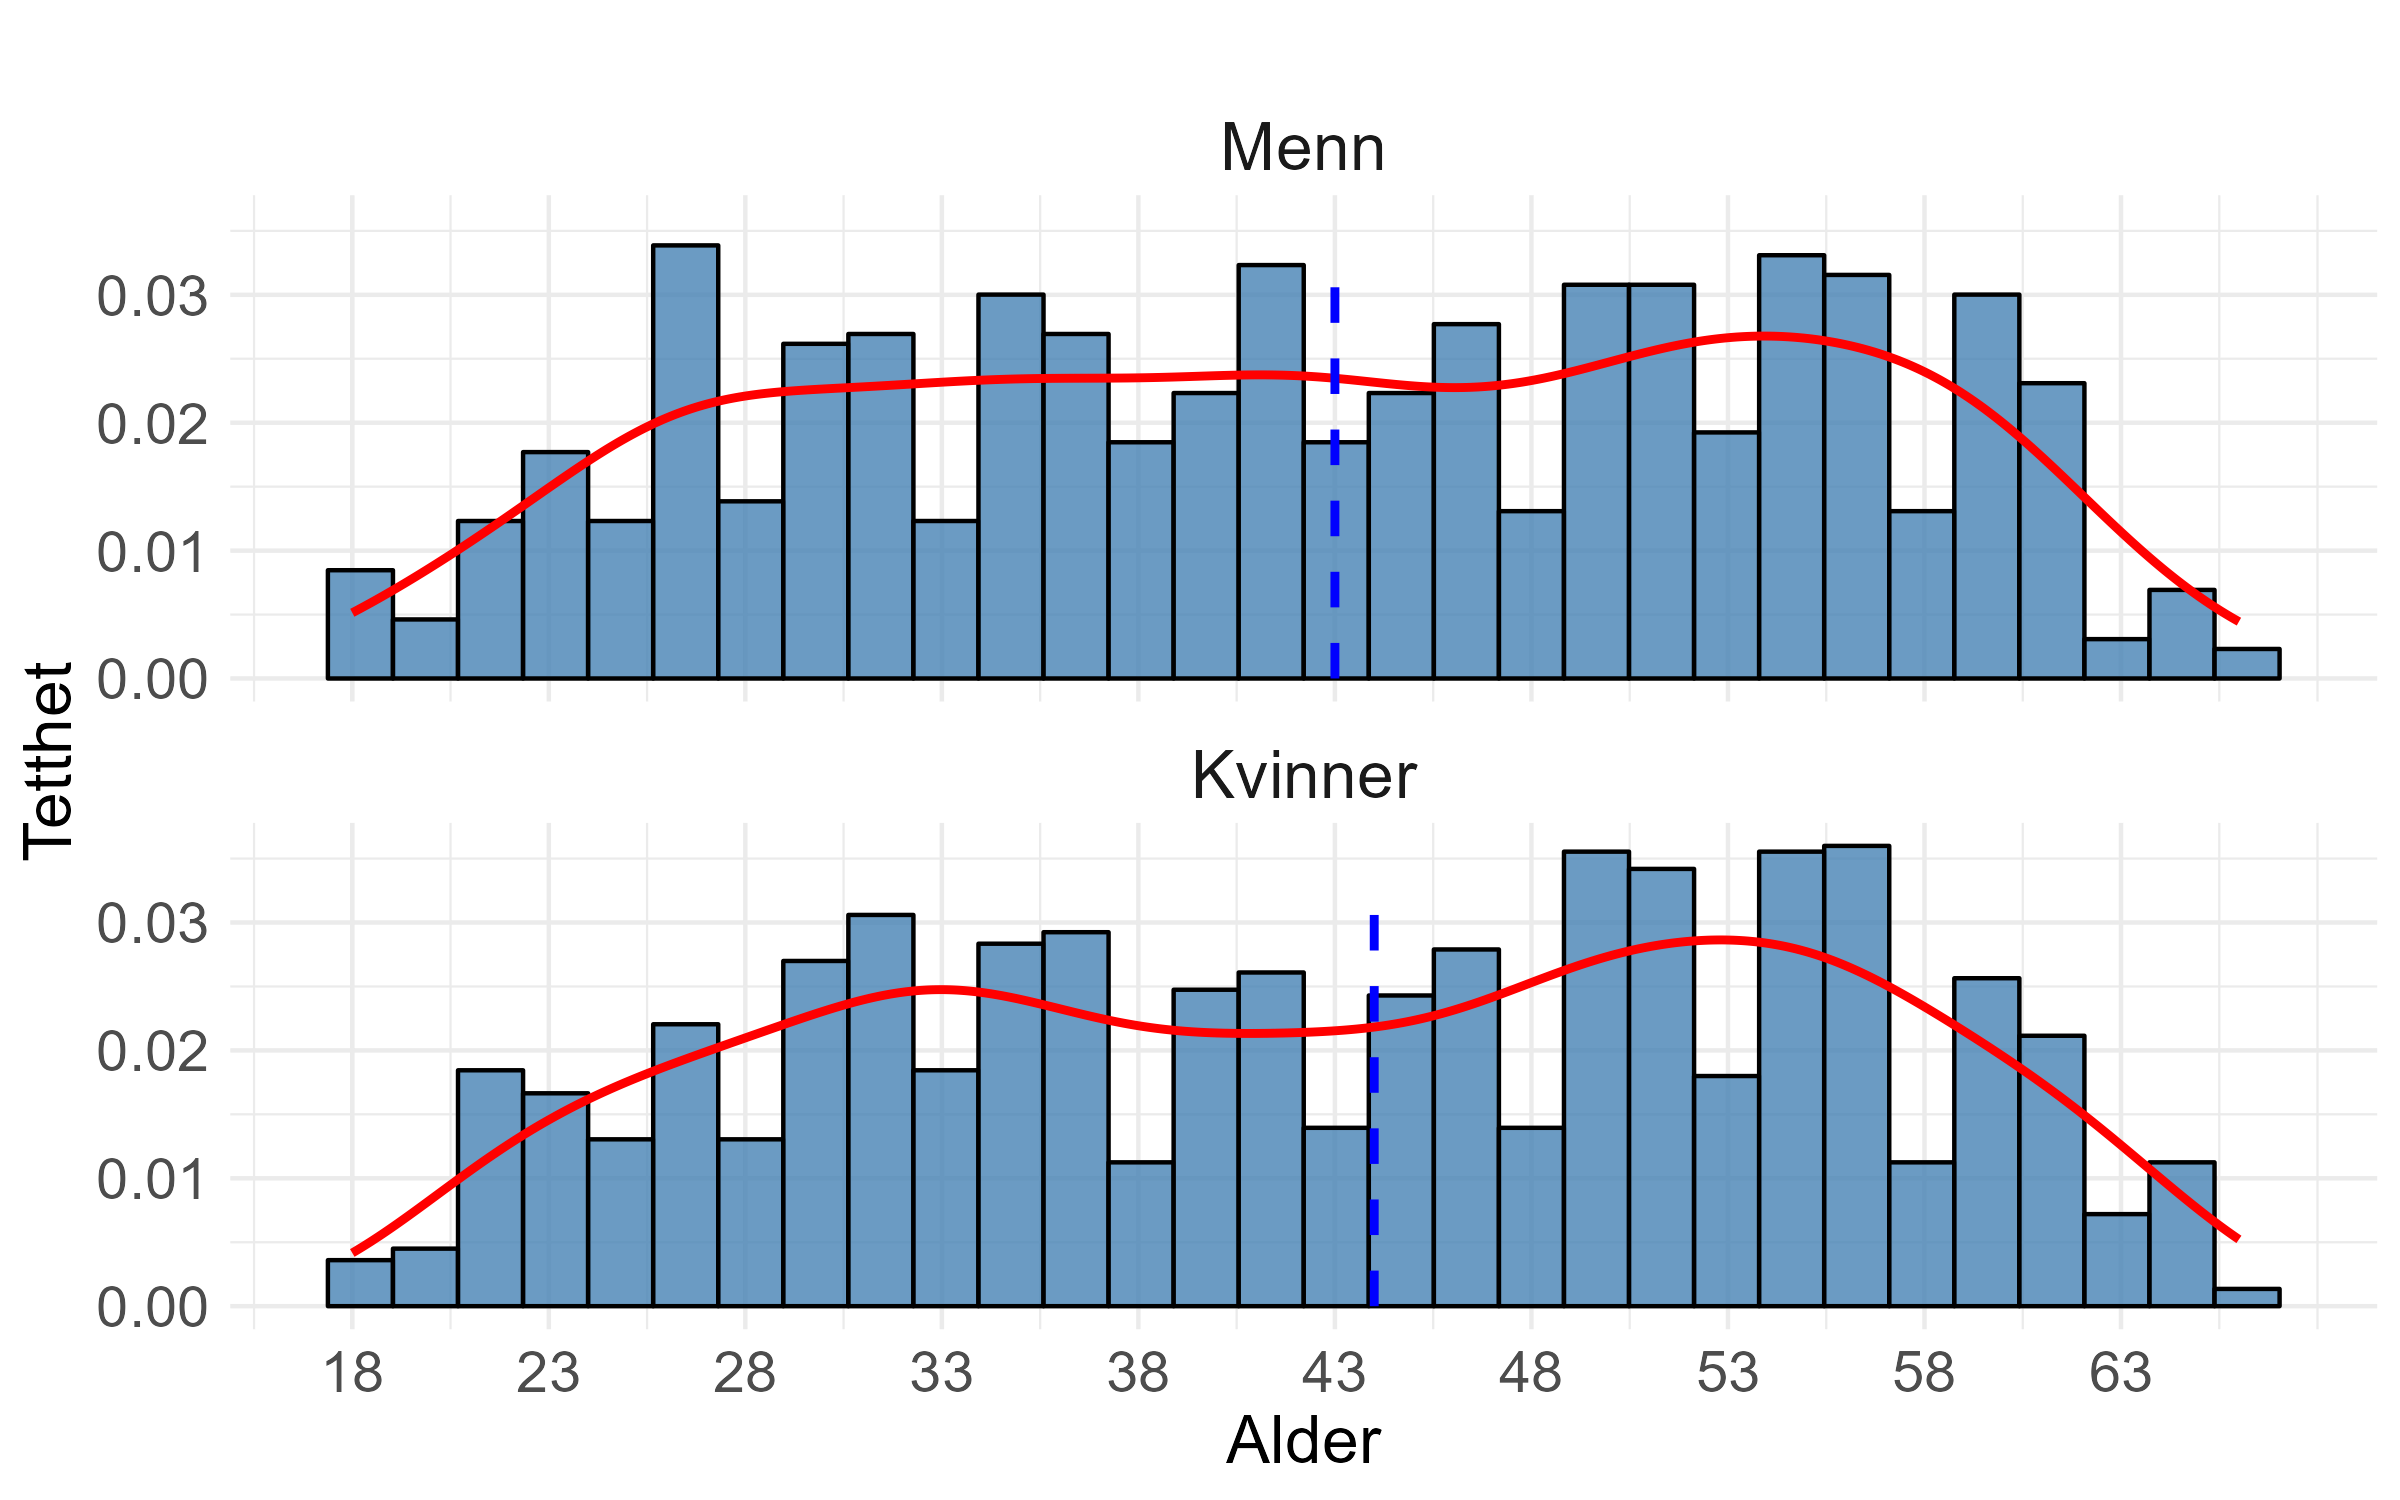
\includegraphics[width=0.8\textwidth]{dokumentobjekter/figurer/fig_2.png}
\end{figure}

\newpage

For analysen så har vi fordelt alder inn i tre breddeintervaller på
18-29, 30-55 og 55-66 år. I \autoref{fig:barplot} presenteres et barplot
av aldersgruppene. Vi har flest respondenter i aldersgruppen 30-54 år
med totalt 59.6 prosent som vi bruker som referansegruppe.

\begin{figure}[H]
\caption{Aldersgruppefordeling}
\label{fig:barplot}
\centering
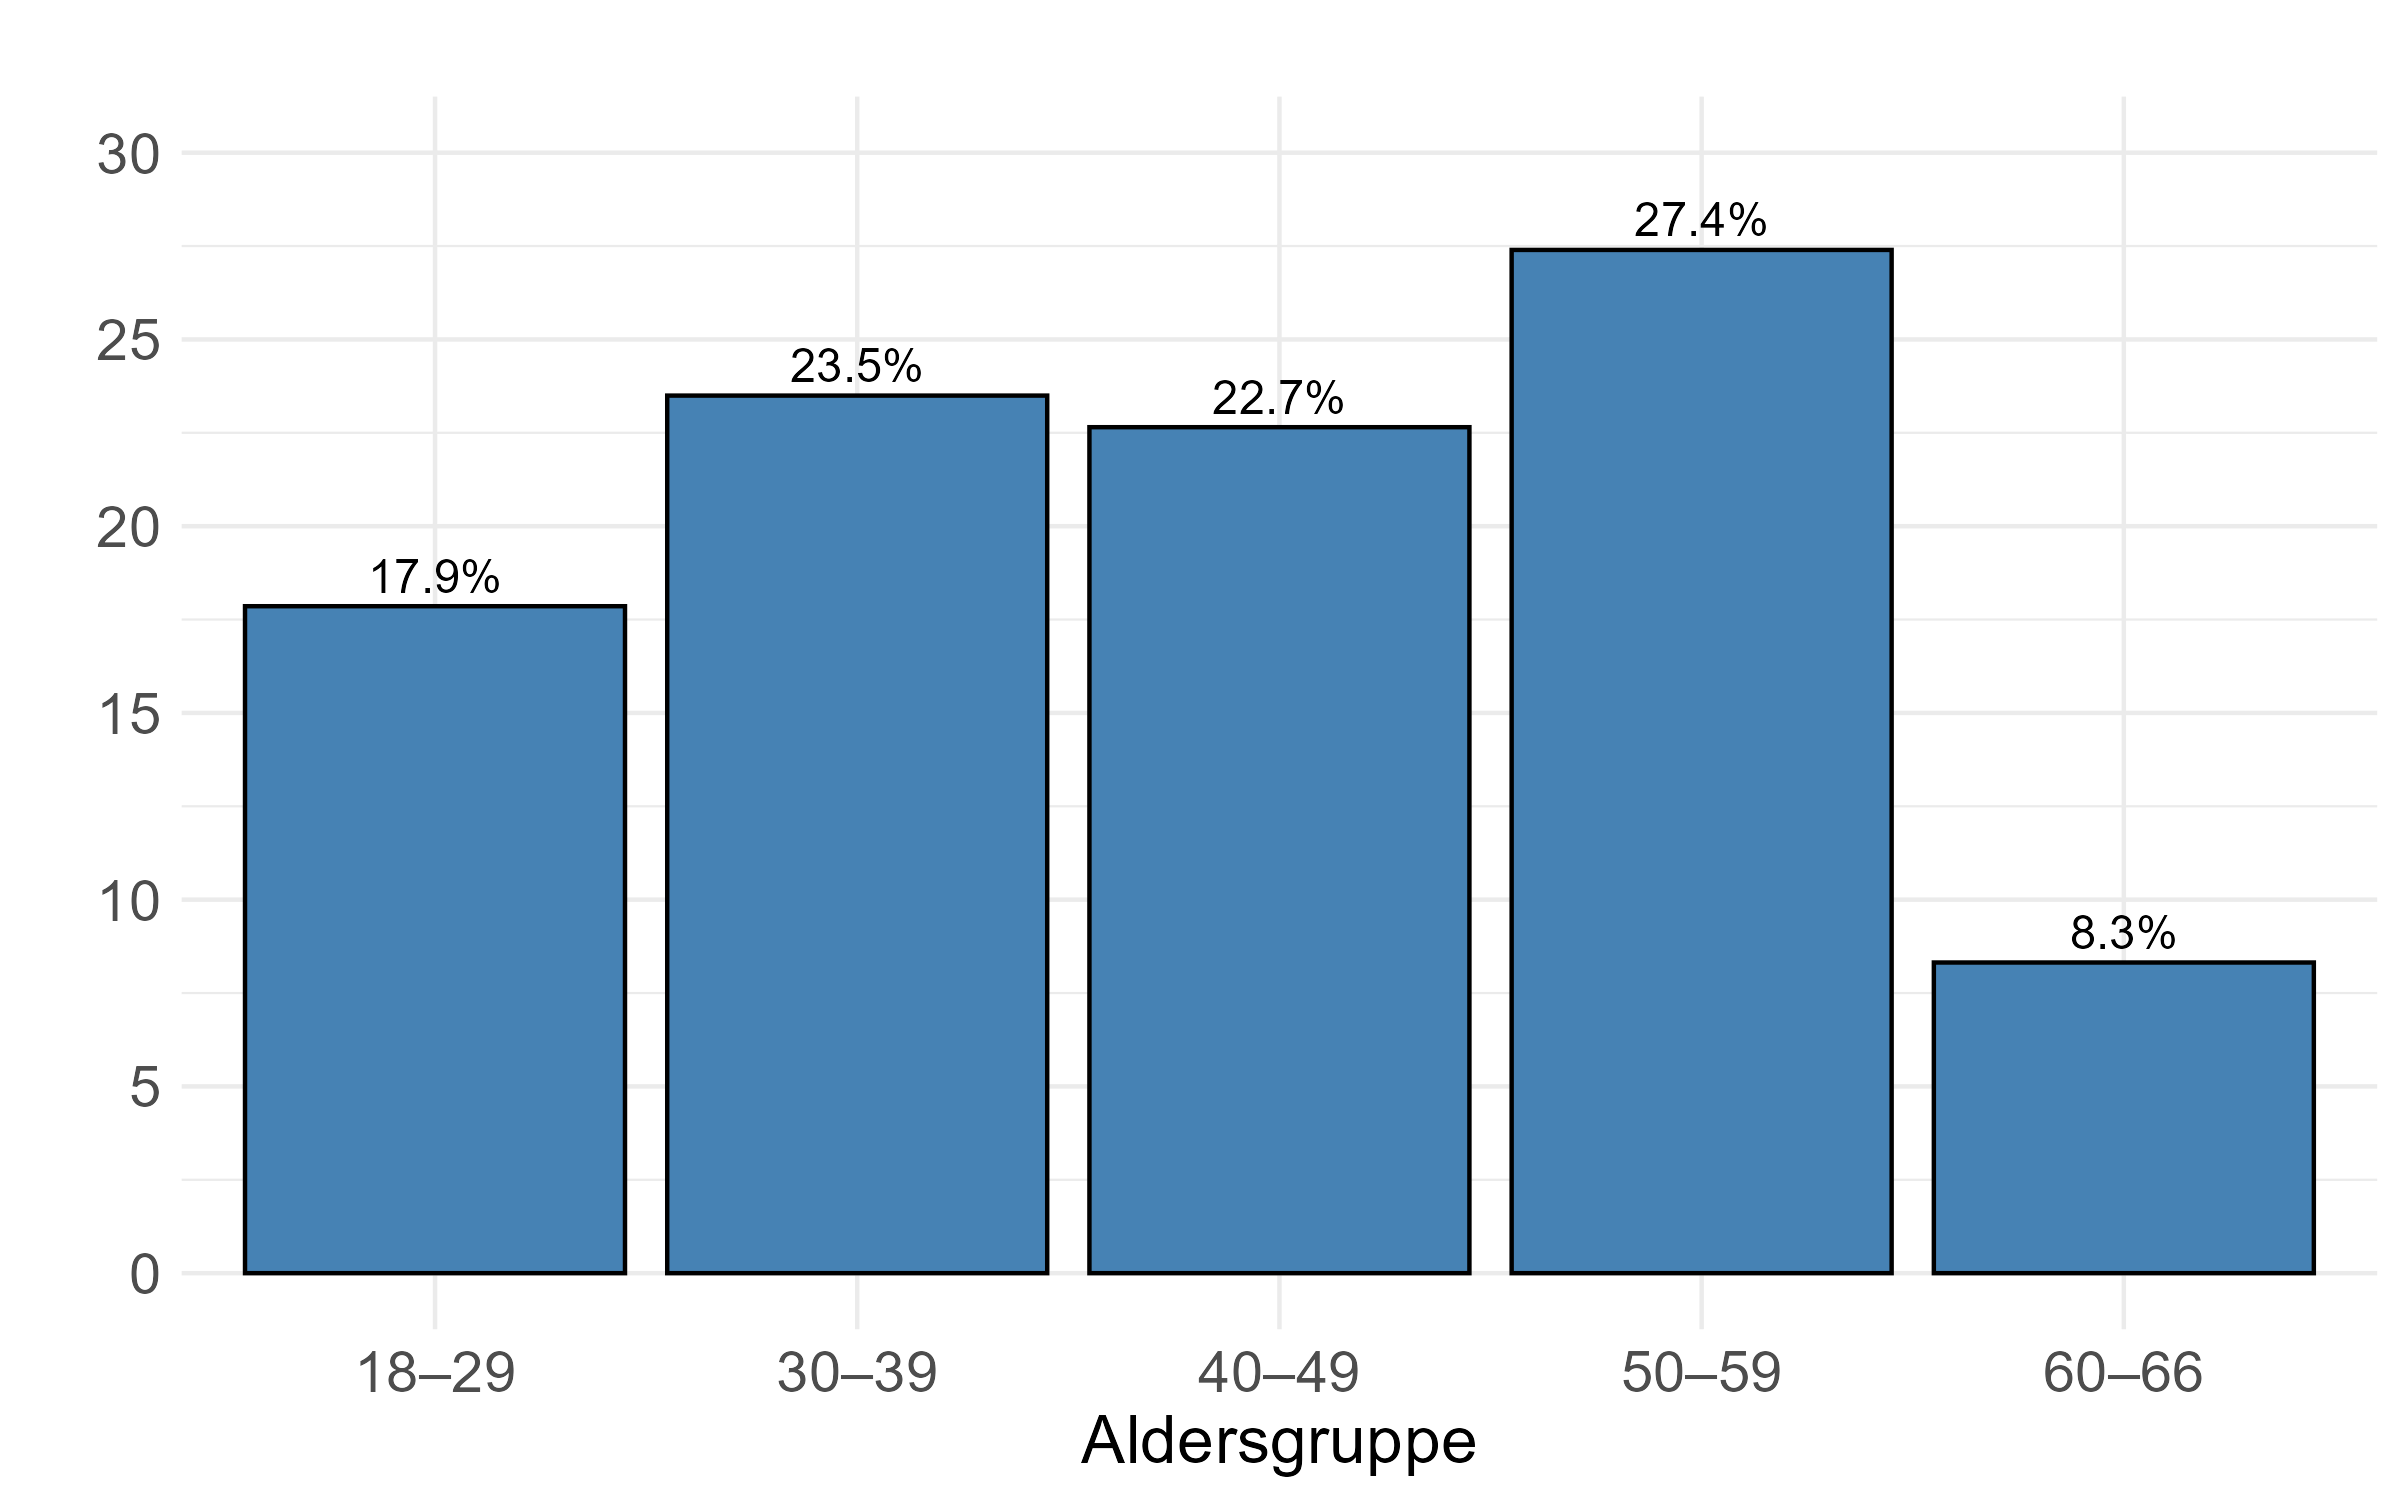
\includegraphics[width=0.8\textwidth]{dokumentobjekter/figurer/fig_3.png}
\end{figure}

I \autoref{fig:histogram_formue} presenteres histogram og tetthetskurve
for bruttofinanskapitalen. Som man kan se er formuefordelingen
høyreskjev både for menn og kvinner, med en høyere andel av
respondentene som har lav formue enn de som har høy formue noe som kan
svekke analysen.

\vspace{-0.5cm}
\begin{figure}[H]
\caption{Fordeling av bruttofinanskapital}
\label{fig:histogram_formue}
\centering
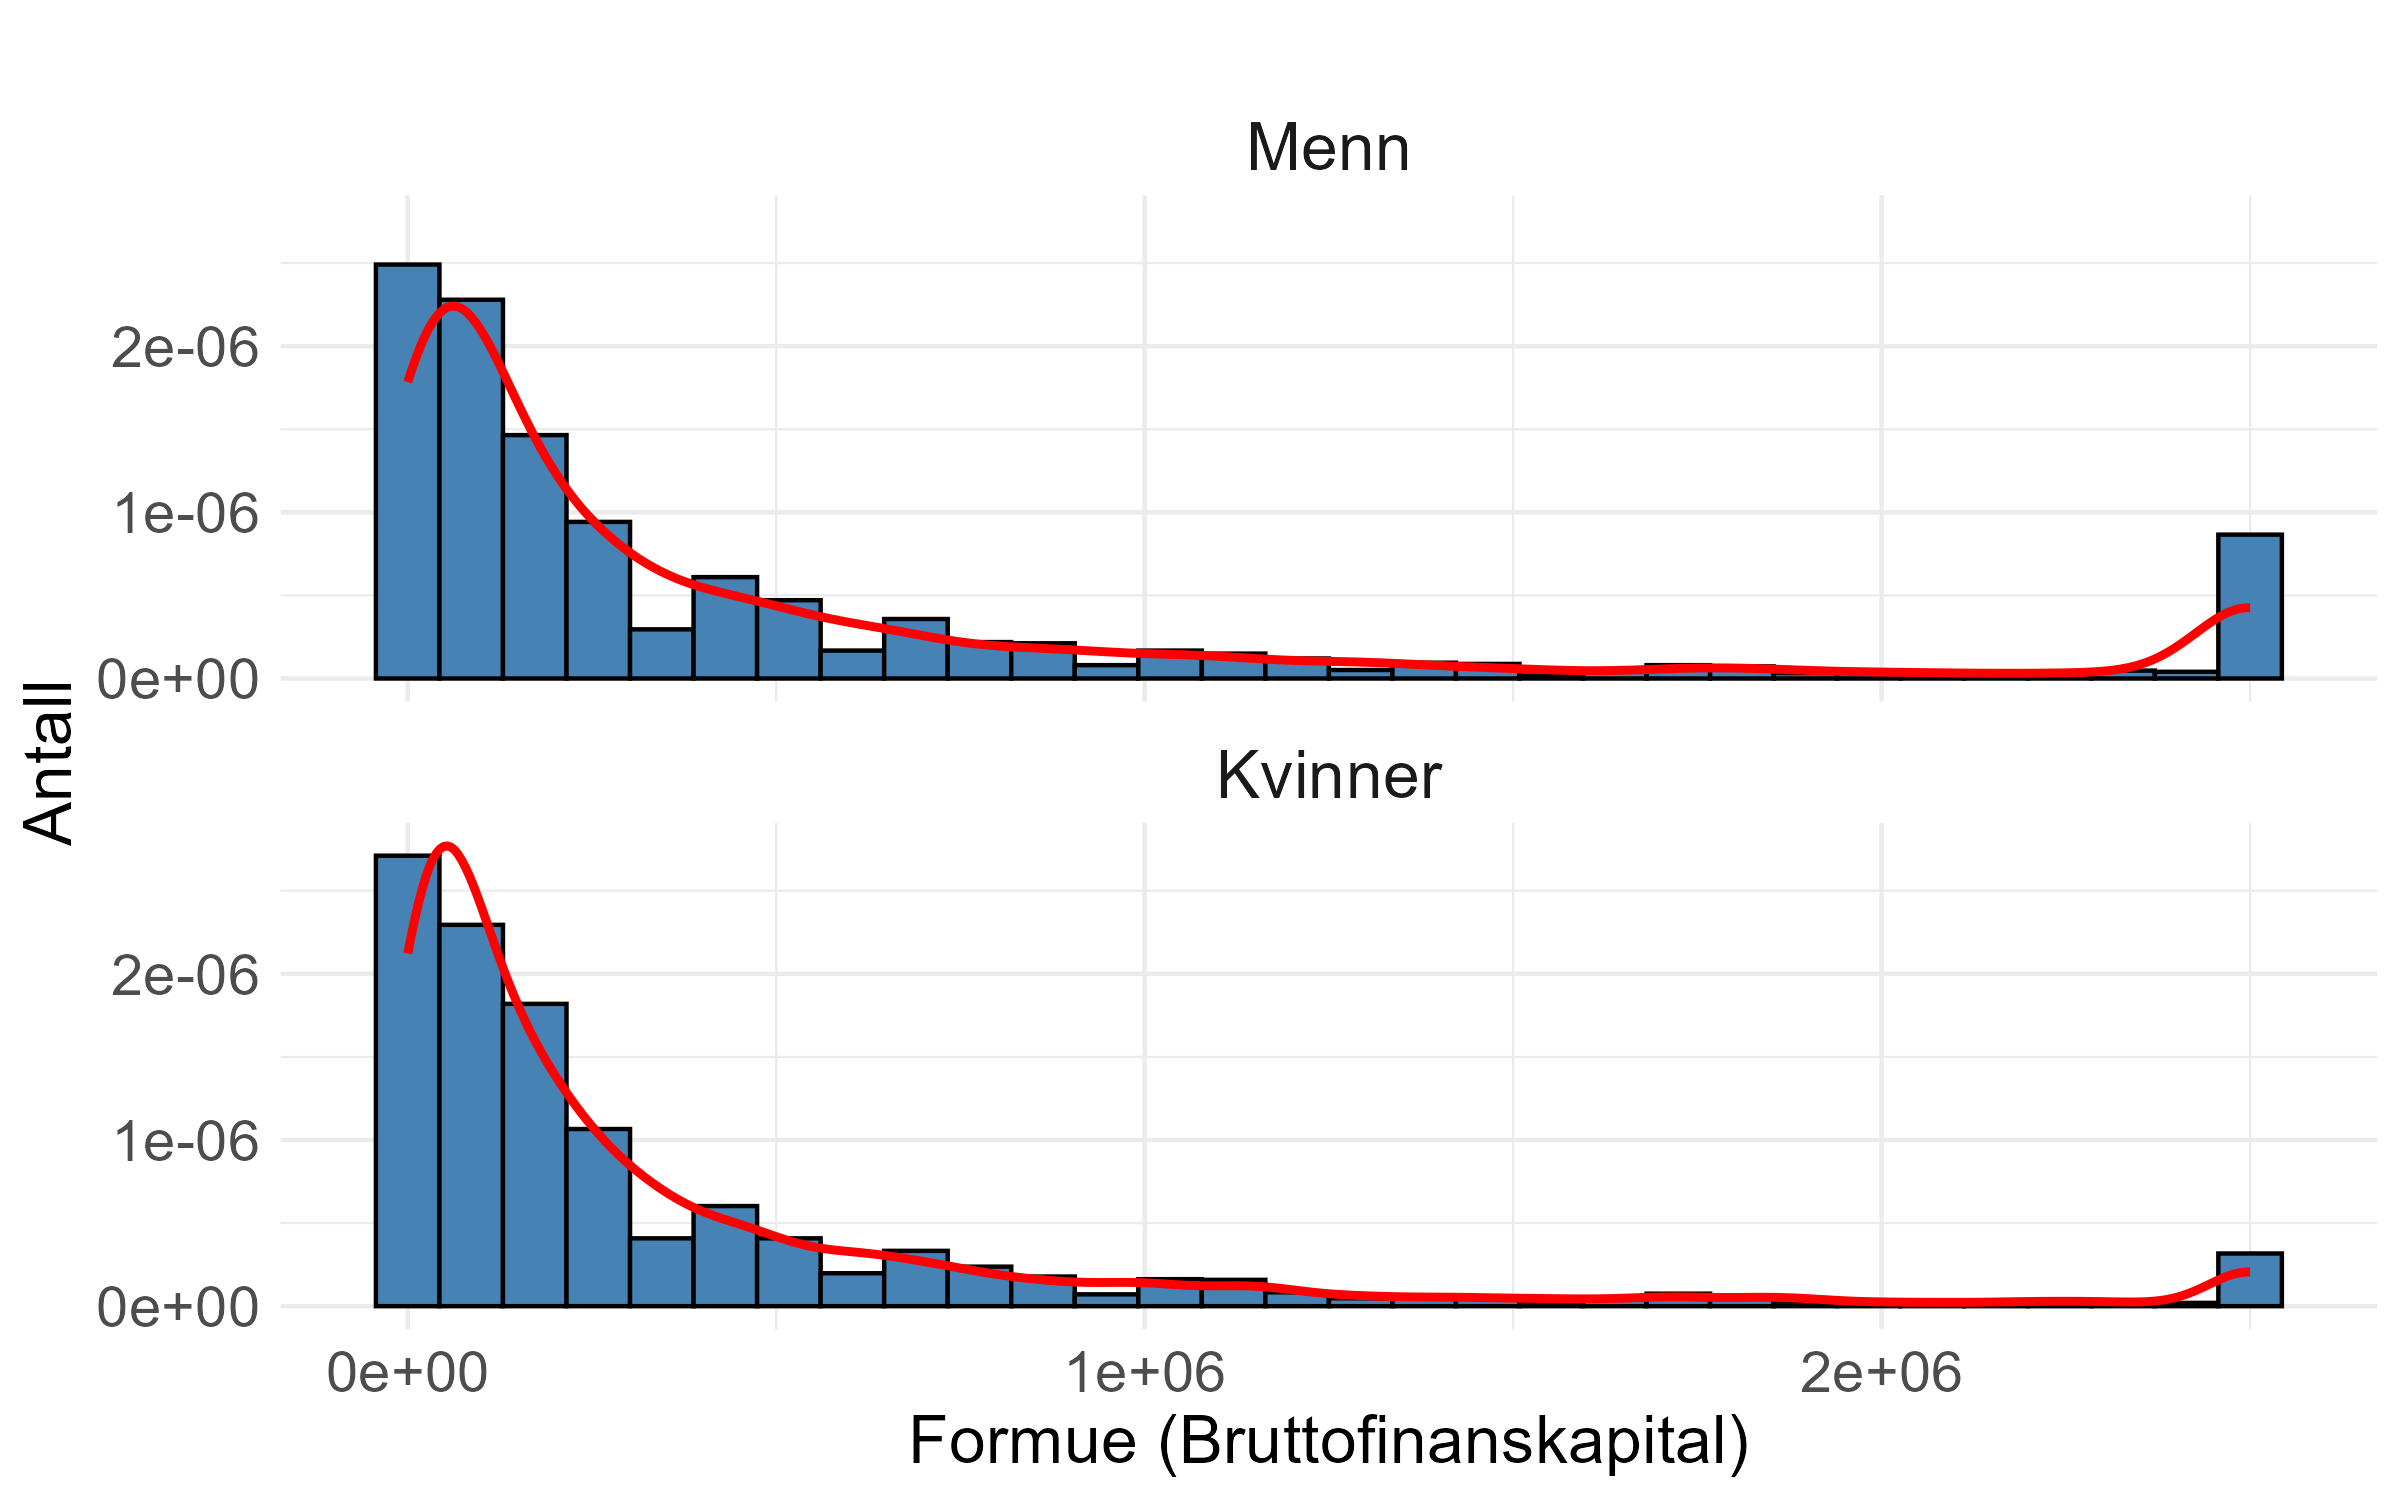
\includegraphics[width=0.8\textwidth]{dokumentobjekter/figurer/fig_4_1.png}
\end{figure}

For å korrigere for denne skjevheten i formuefordelingen må vi gjøre en
invertering av den kumulative fordelingen av bruttofinanskapitalen. Som
man kan se i \autoref{fig:histogram_formue_fordeling} så er den
inverterte kumulative fordelingen av bruttofinanskapitalen mer
normalfordelt, noe som gjør at vi kan bruke den i analysen vår.

\vspace{-0.75cm}
\begin{figure}[H]
\caption{Invertert kumulativ fordeling av bruttofinanskapital}
\label{fig:histogram_formue_fordeling}
\centering
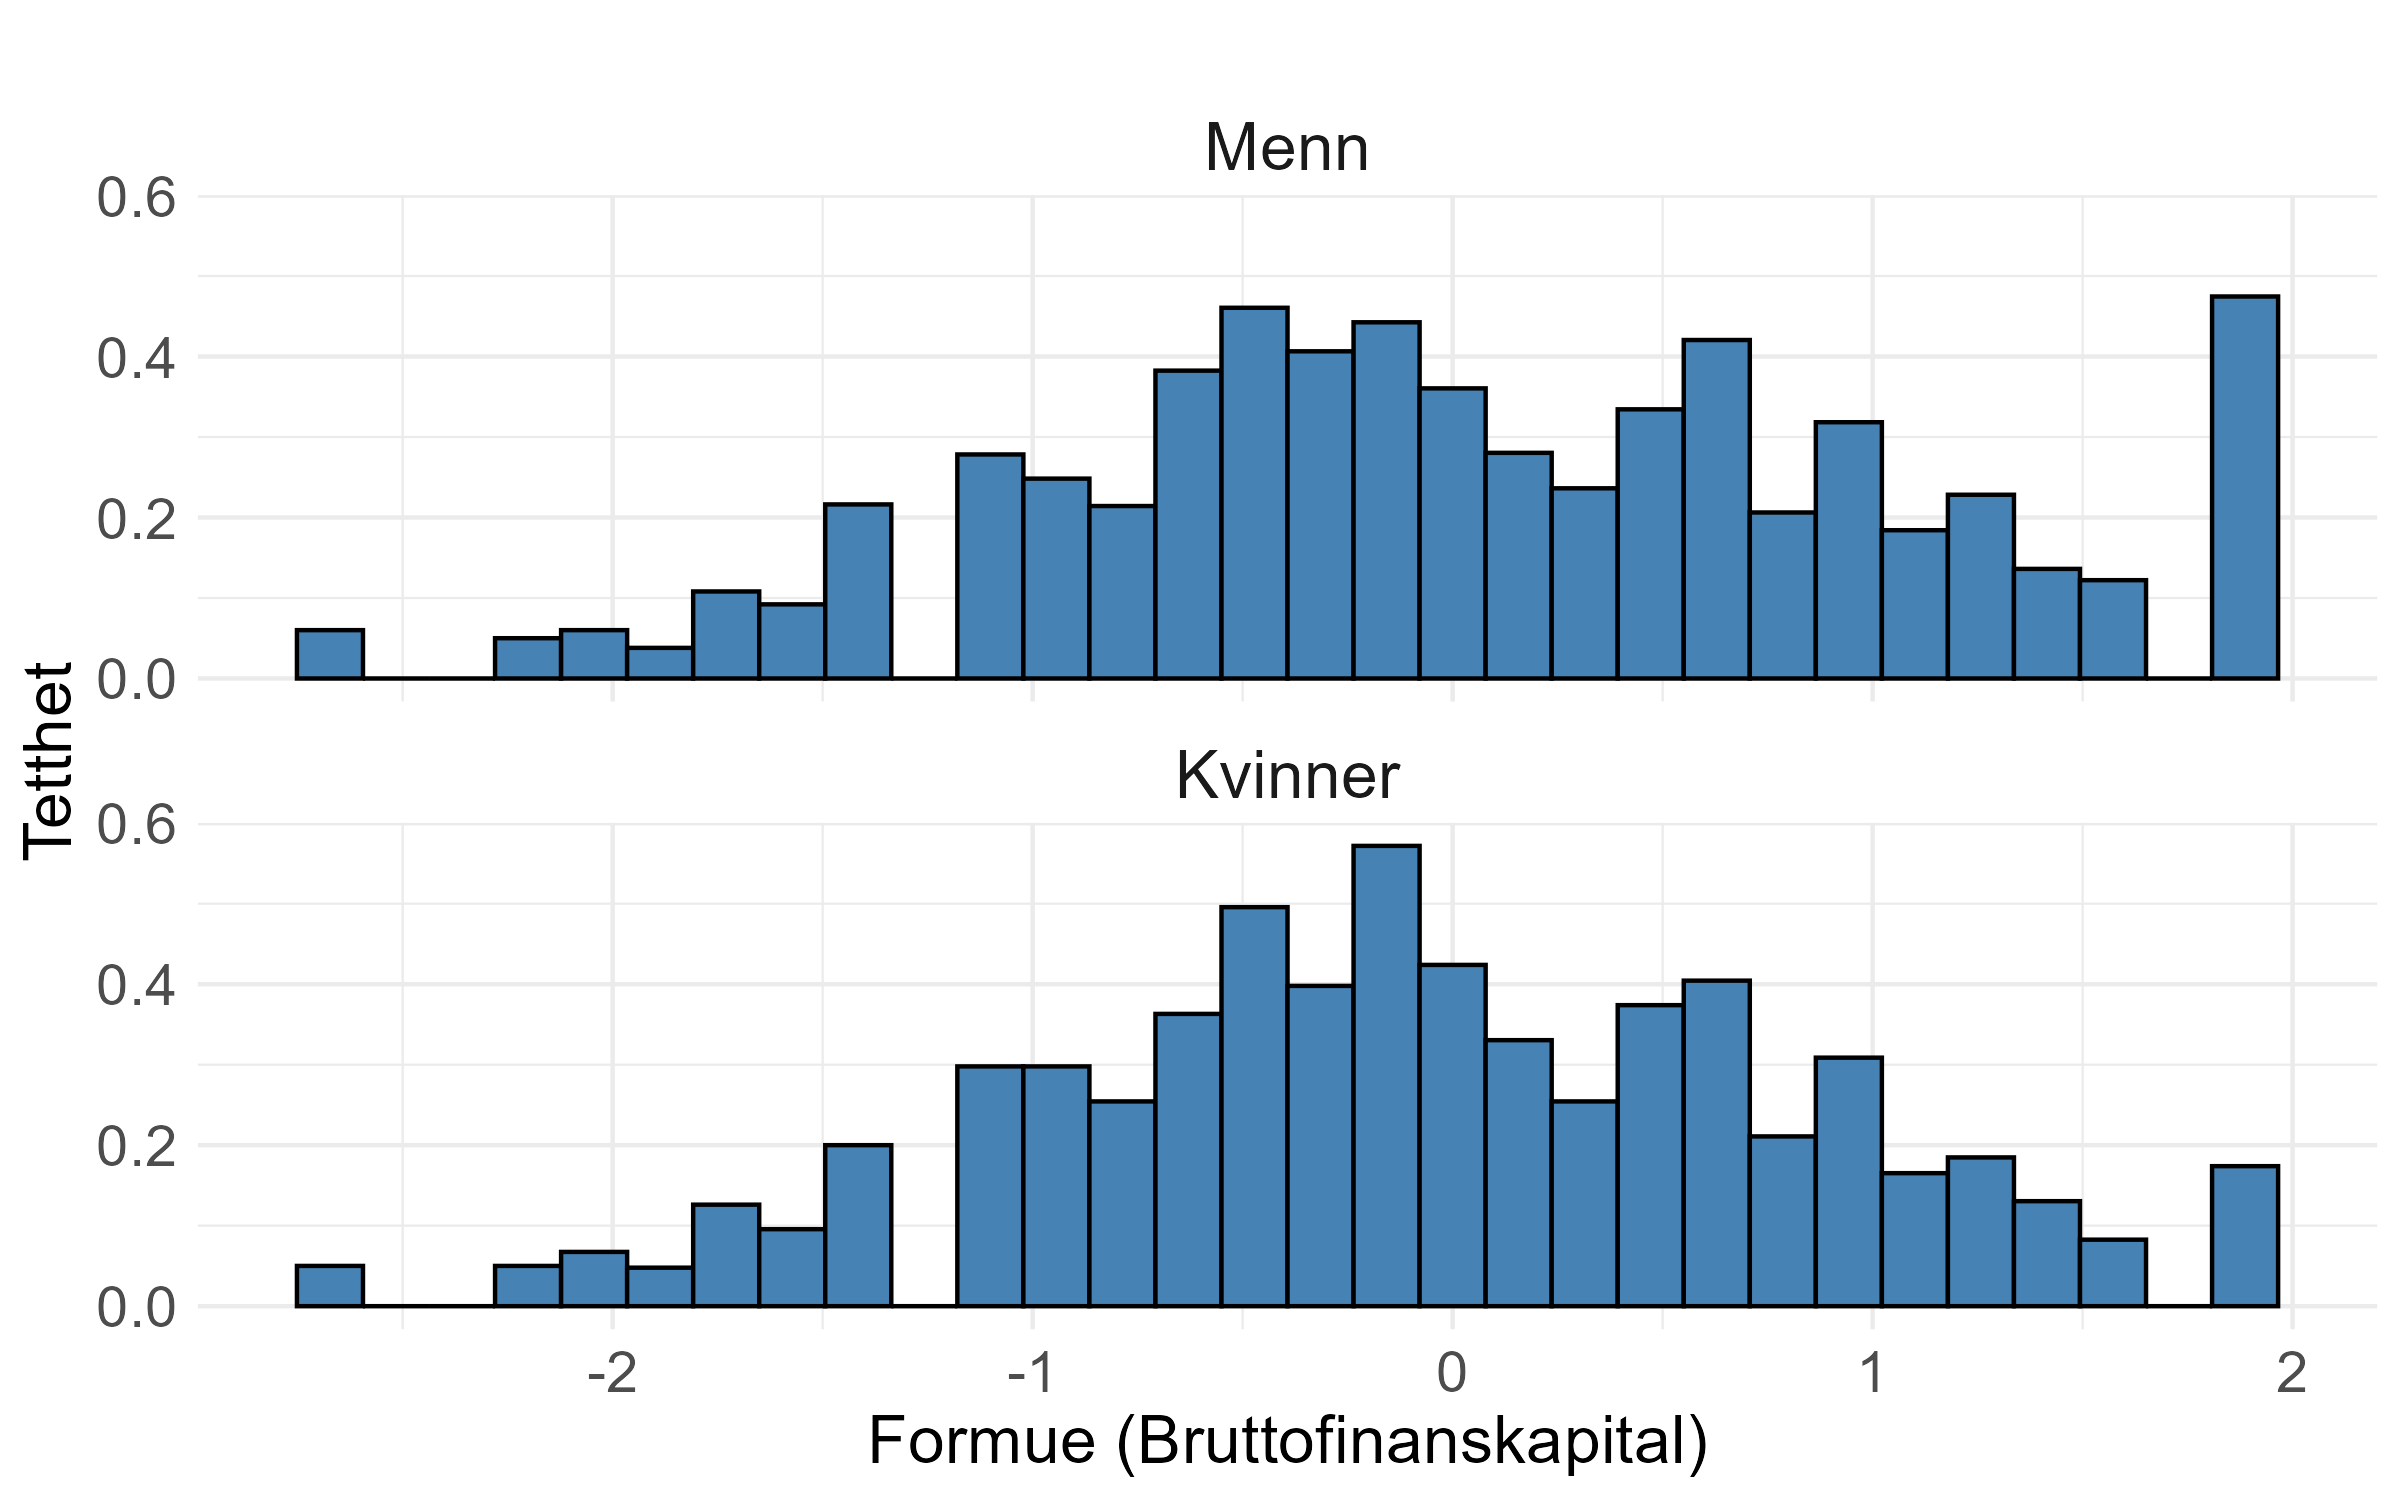
\includegraphics[width=0.8\textwidth]{dokumentobjekter/figurer/fig_4_2.png}
\end{figure}
\vspace{-0.75cm}

Når vi ser på fordelingen av utdanningsgrupper fordelt på kjønn i
\autoref{fig:barplot_2} så ser vi at det er flest menn i
utdanningsgruppen videregående skole med 53.7 prosent, mens kvinner har
noe lavere med 42.3 prosent. Mer kvinner enn menn har
universitetsutdannings eller høyskole med 46.7 prosent mot 30.8 prosent
for menn. Menn har også lavest utdanningsnivå med 15.5 prosent i
utdanningsgruppen grunnskole eller mindre, mens kvinner har 11 prosent i
den samme utdanningsgruppen. Menn har lavere utdanningsnivå enn kvinner,
og kvinner er mer tilbøyelige til å ta høyere utdanning.

\vspace{-0.5cm}
\begin{figure}[H]
\caption{Fordeling av utdanningsgrupper fordelt på kjønn}
\label{fig:barplot_2}
\centering
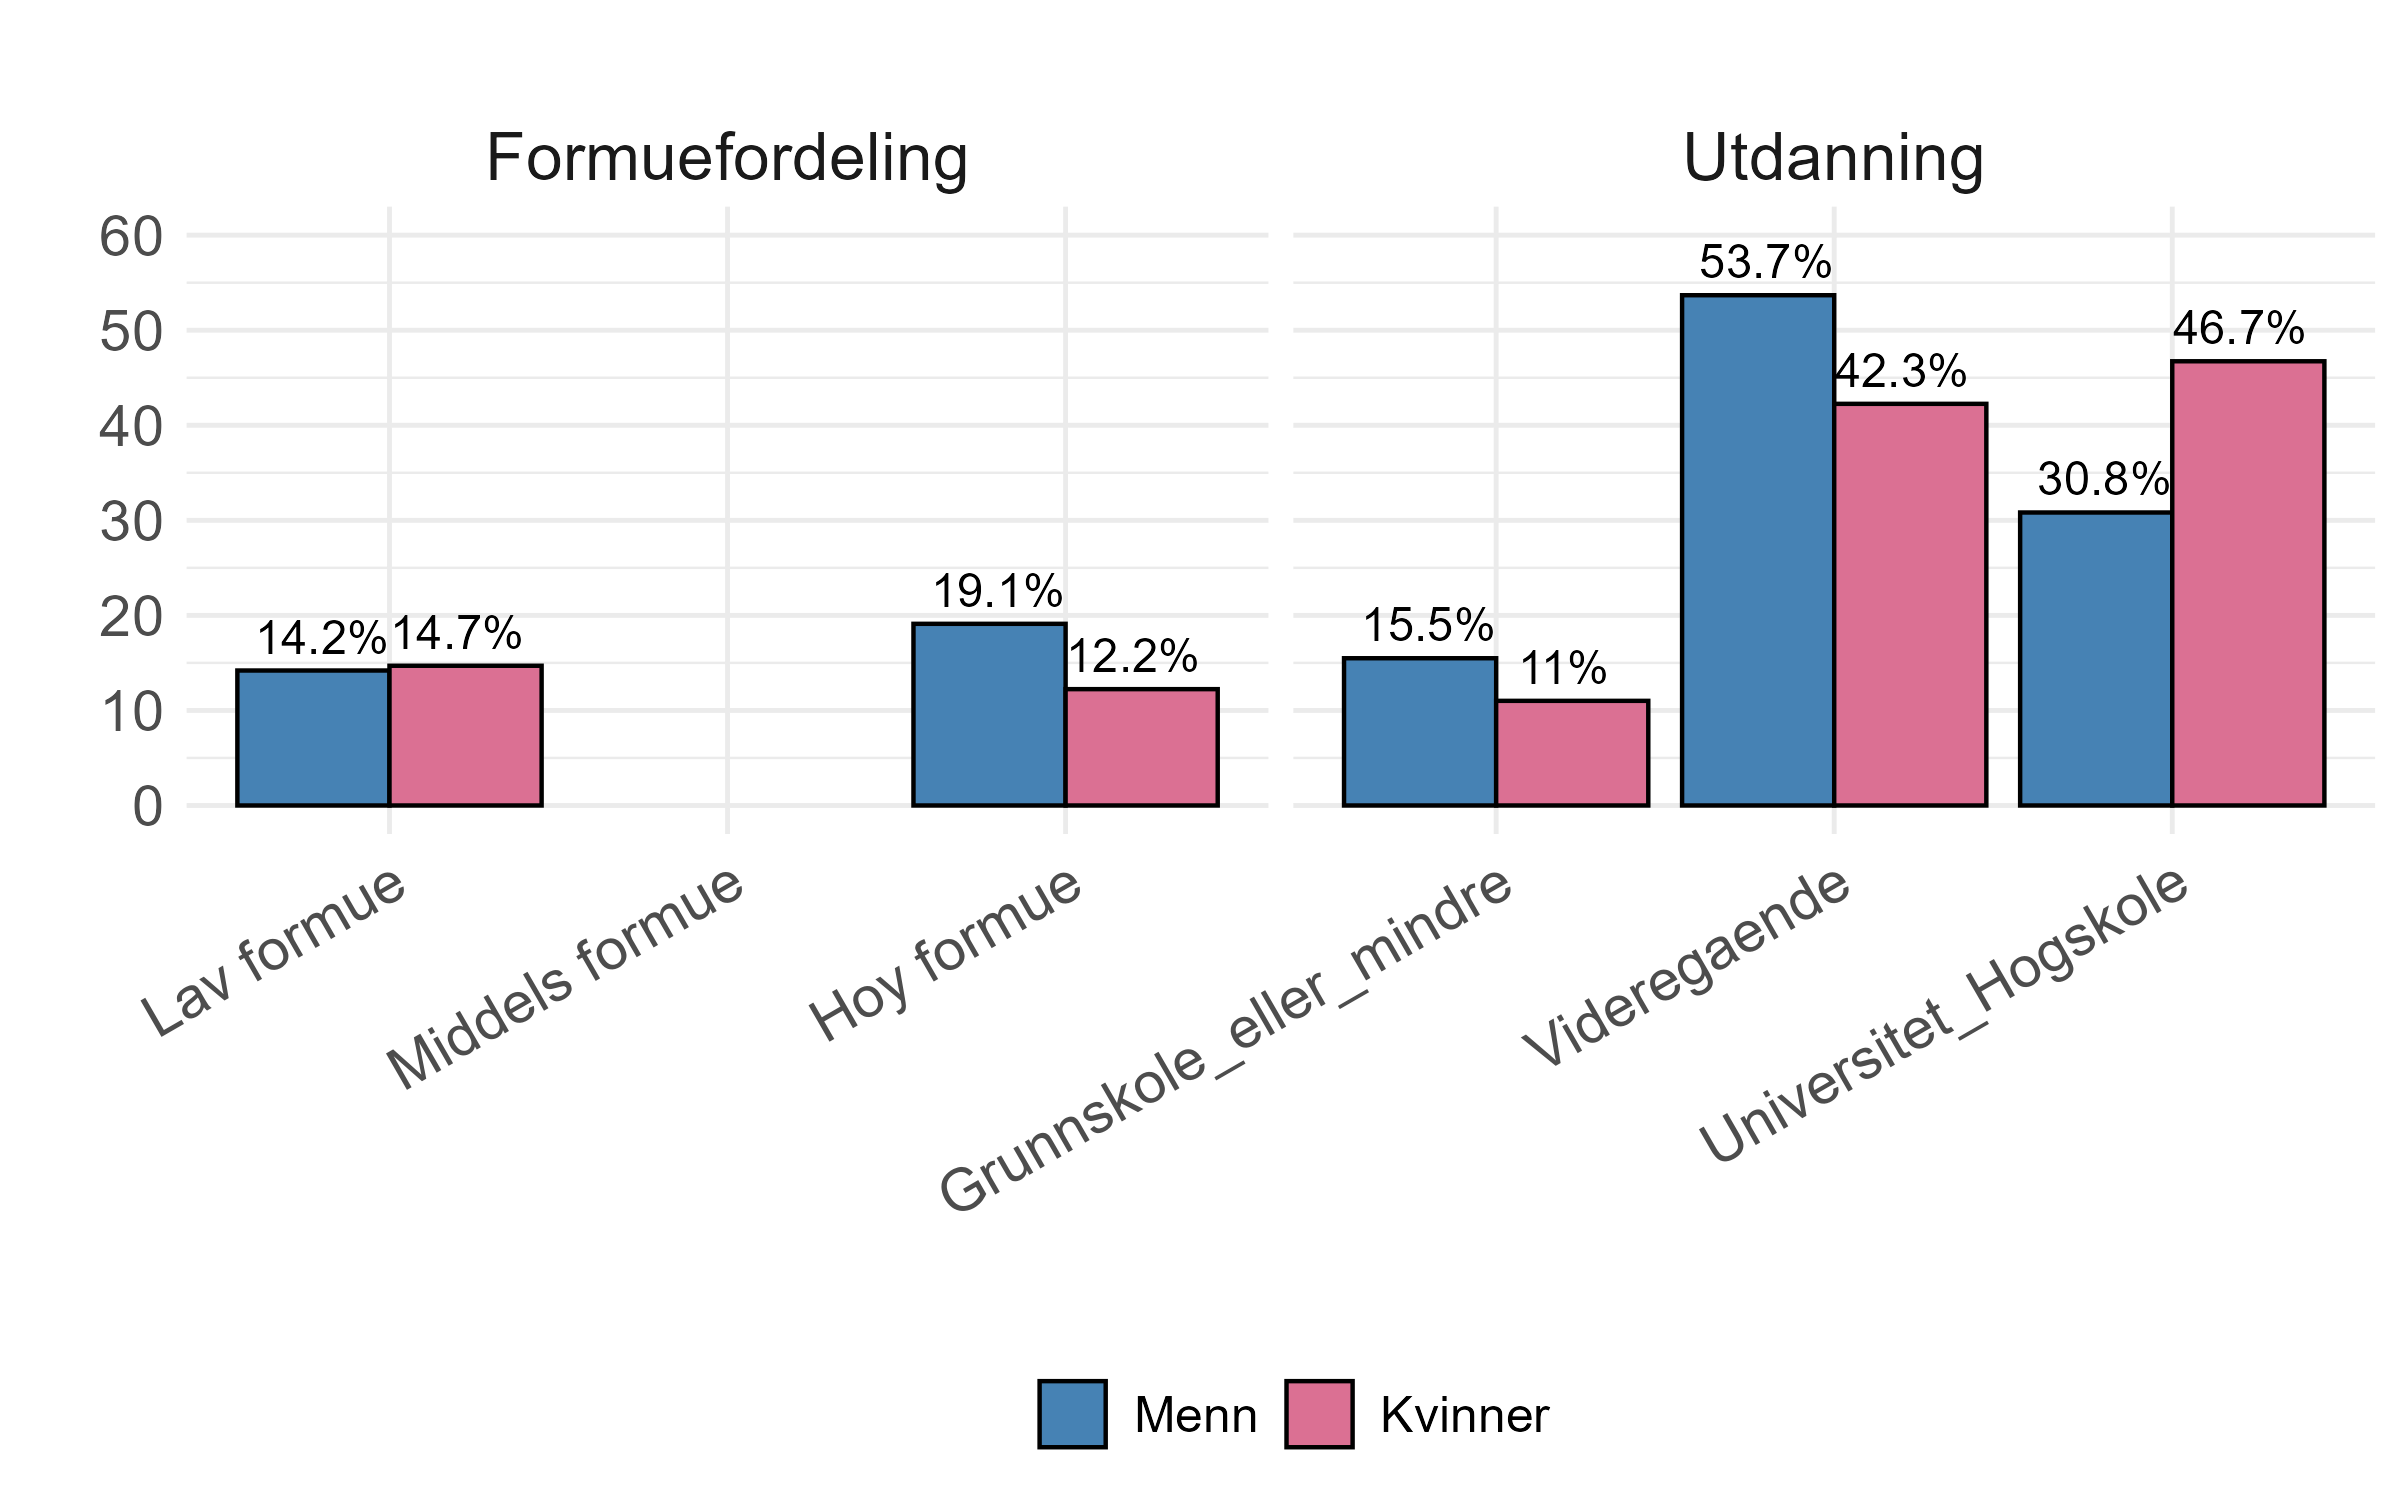
\includegraphics[width=0.75\textwidth]{dokumentobjekter/figurer/fig_5.png}
\end{figure}
\vspace{-1cm}

I \autoref{fig:boxplot} presenteres et boksplott av sykefravær etter
formuegrupper som er definert etter standardavvik fra gjennomsnittet. Vi
har tre formuegrupper: lav formue (under 1 standardavvik under
gjennomsnittet), middels formue (mellom 1 standardavvik under og over
gjennomsnittet) og høy formue (over 1 standardavvik over
gjennomsnittet).

Vi kan se at det er en liten trend i sykefraværet etter formuegruppe,
der de med høy formue har lavest sykefravær, mens de med lav formue har
høyest sykefravær. Dette er i tråd med hypotesen vår om at formue kan
påvirke sykefraværet.

Medianen vises i den sorte streken i midten av boksen, og den viser at
sykefraværet med små marginer går ned fra lav formue, til middels formue
og til høy formue. Bunnen og toppen til boksene viser oss henholdsvis
første og tredje kvartil, og de stiplede linjene viser oss minimum og
maksimum sykefravær. Det er også noen uteliggere som er vist med små
prikker, og de viser at det er noen respondenter som har rapportert
sykefravær på over 40 prosent. Dette kan være at de har vært sykemeldt i
en lengre periode. I bakgrunnen av figuren man man se alle
observasjonene spredt utover for en bedre oversikt siden det er mange
observasjoner som går over hverandre i boksen. Dette er gjort med en
funksjon som sprer ut observasjonene litt for å få en bedre oversikt
over dem.

I analysen bruker vi ikke formuegruppene, men figuren inkluderes for å
få en bedre oversikt over hvordan sykefraværet fordeler seg etter
formue.

\begin{figure}[H]
\caption{Boksplott av sykefravær etter formuegruppe}
\label{fig:boxplot}
\centering
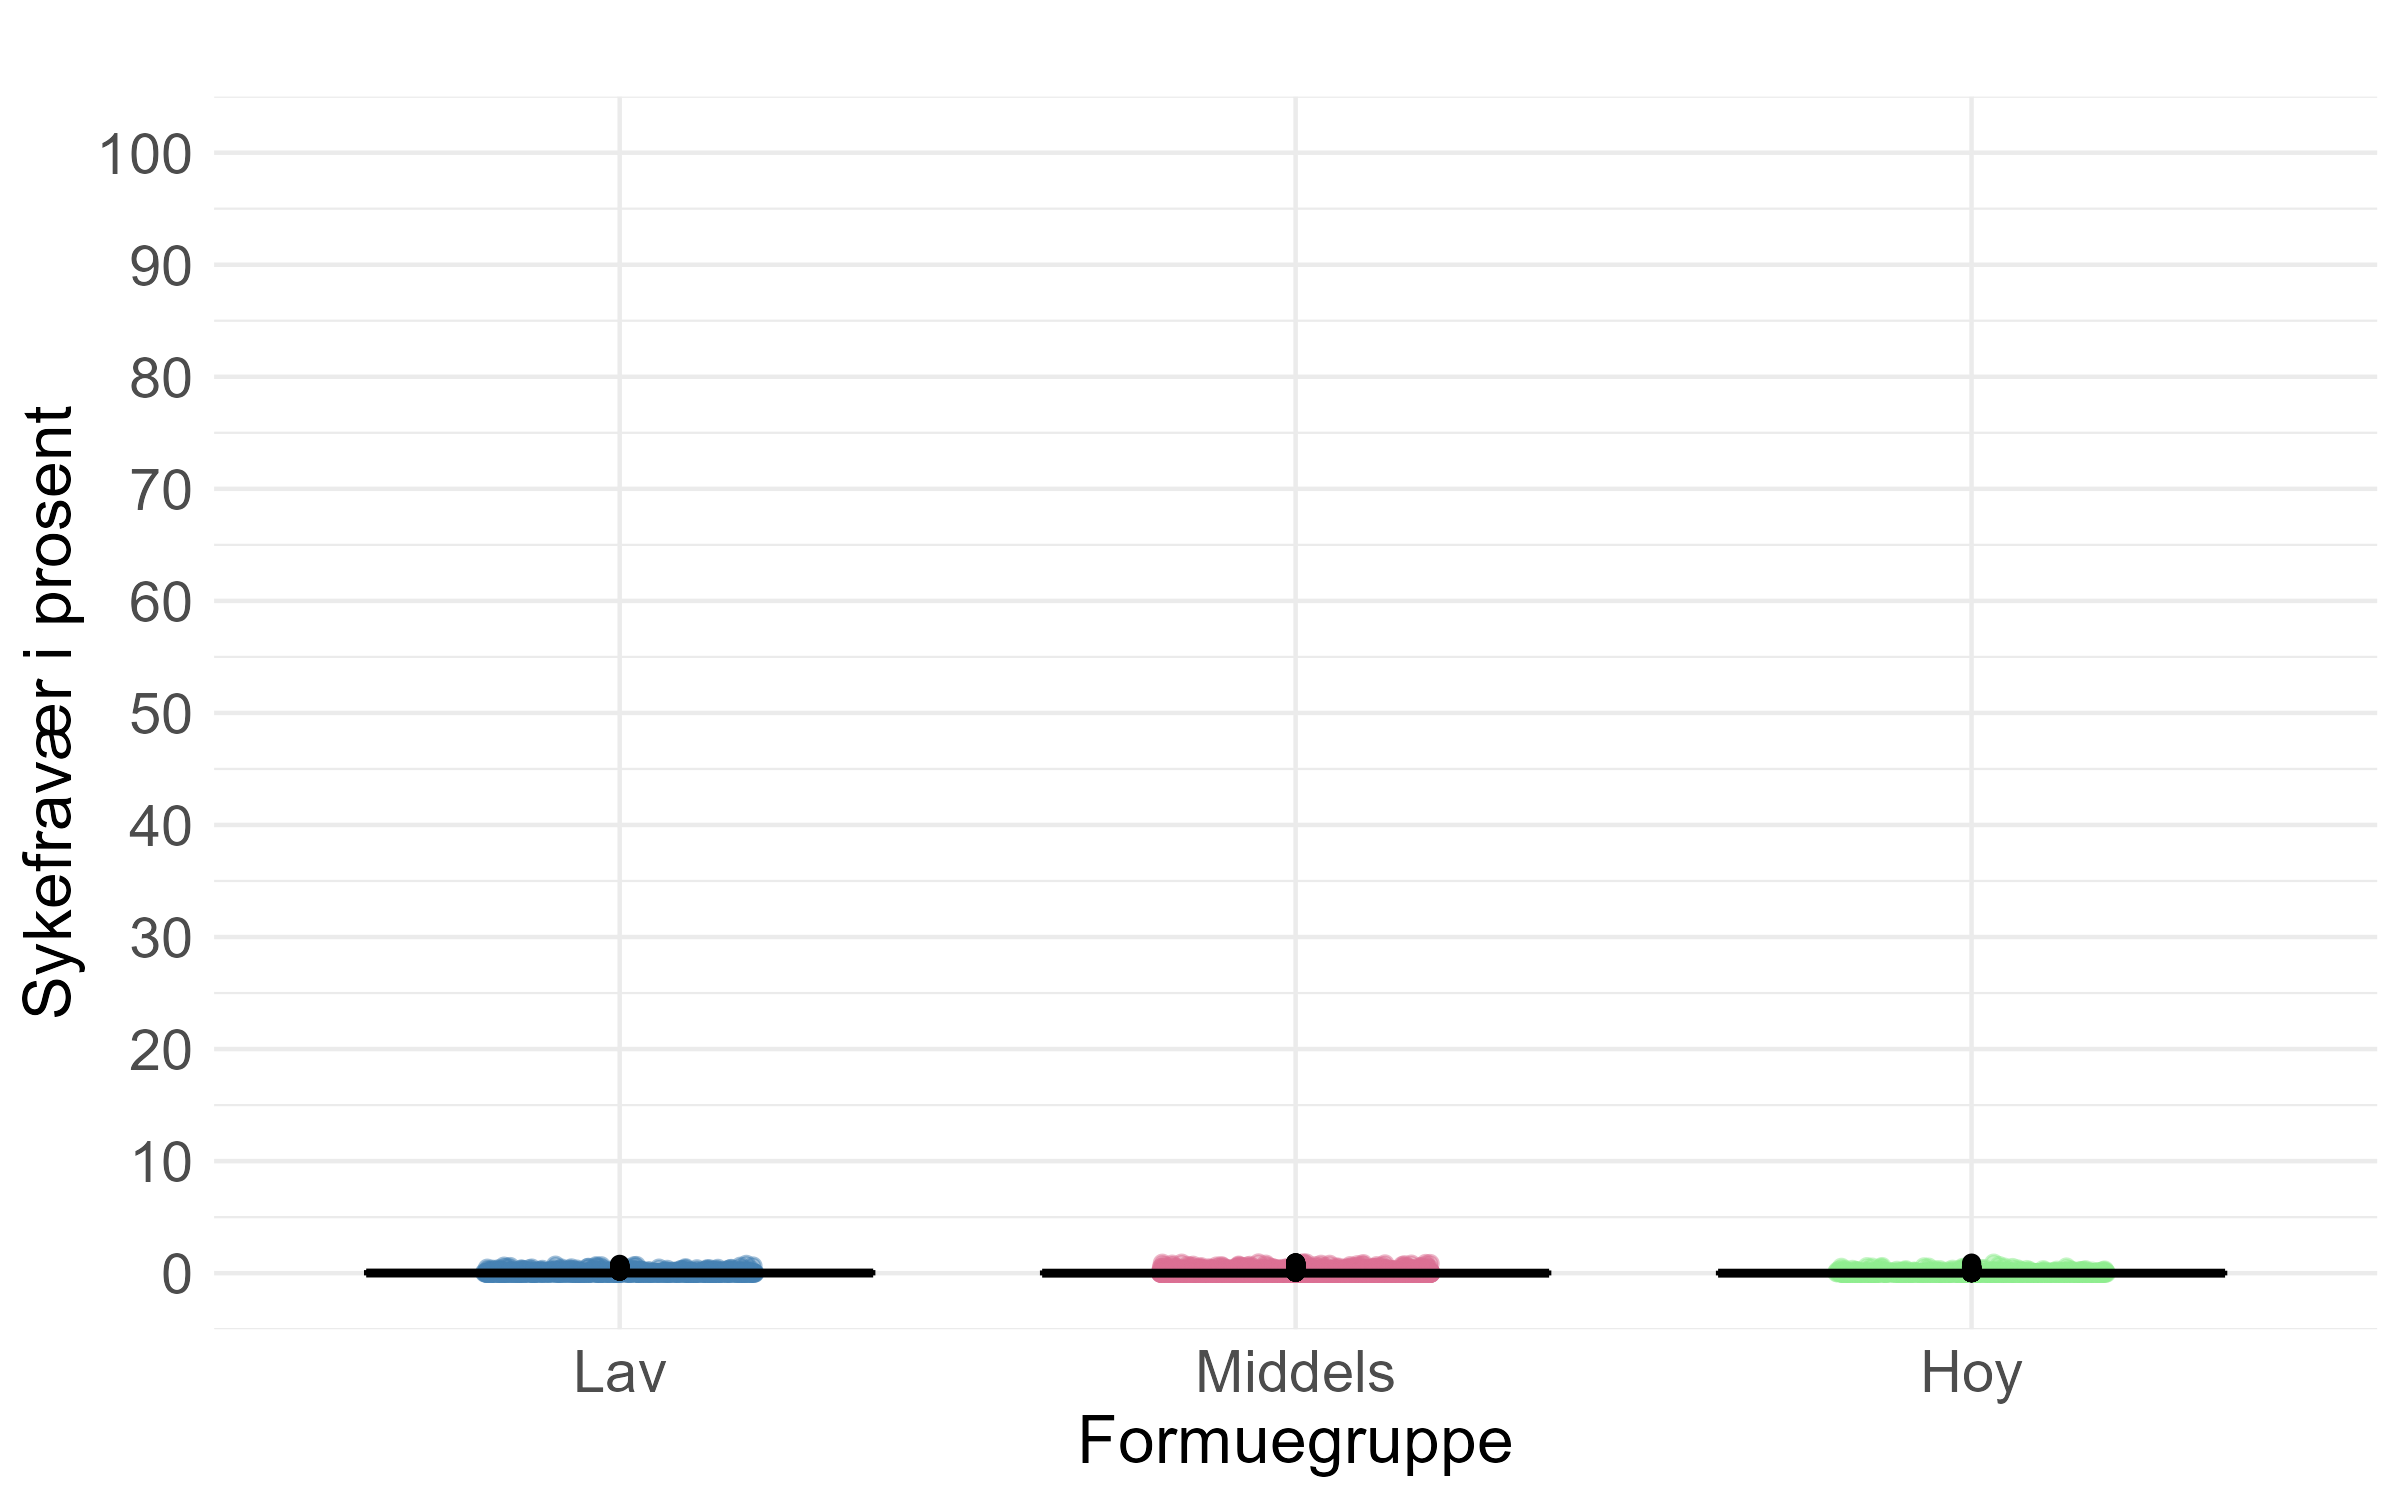
\includegraphics[width=0.8\textwidth]{dokumentobjekter/figurer/fig_6.png}
\end{figure}

\newpage

I \autoref{fig:boxplot_2} presenteres et boksplott av sykefravær etter
utdanningsnivå. Vi ser at sykefraværet er relativt jevnt mellom
utdanningsnivåene, og som tidligere vet vi at gjennomsnittlig sykefravær
er lavere for høyt utdannede og litt høyere for de med lavere utdanning.

\vspace{-0.5cm}
\begin{figure}[H]
\caption{Boksplott av sykefravær etter utdanningsnivå}
\label{fig:boxplot_2}
\centering
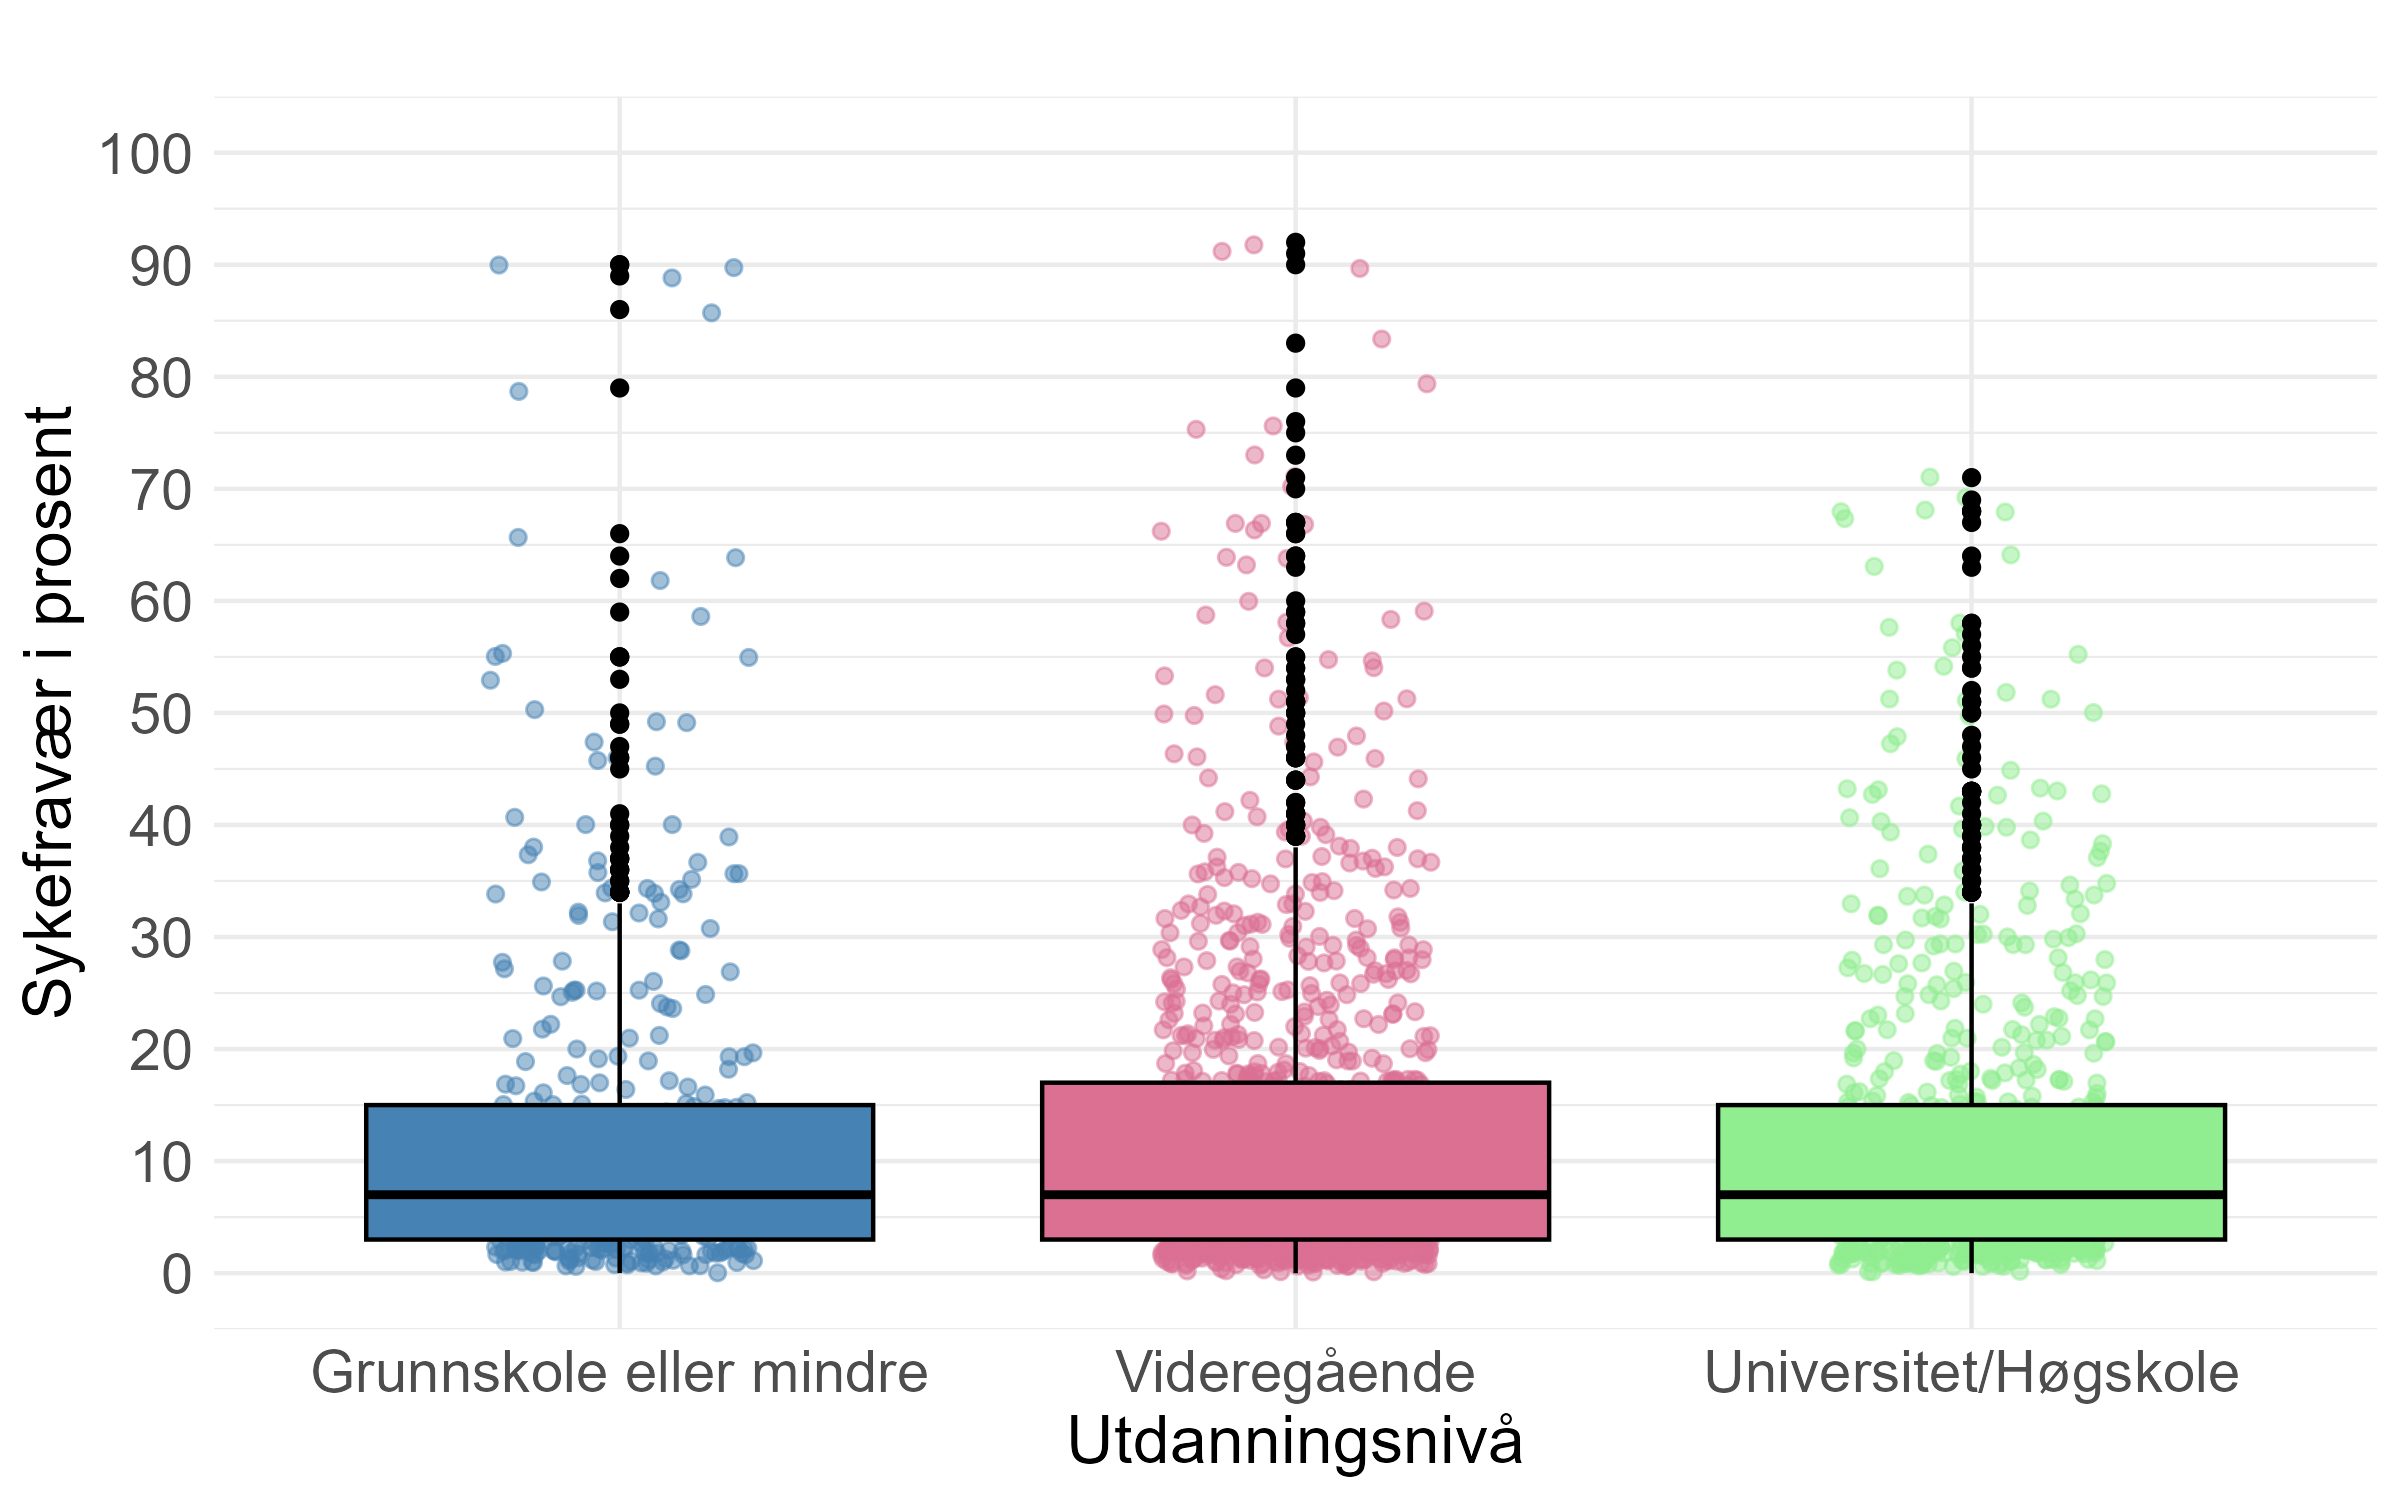
\includegraphics[width=0.8\textwidth]{dokumentobjekter/figurer/fig_7.png}
\end{figure}
\vspace{-1cm}

I \autoref{fig:kontrollvariabler} presenteres fordelingen av de
arbeidsrelaterte variablene som inngår i de latente variablene jobbkrav
og jobbressurser samt motivasjon. Vi ser at det er en høy andel som
rapporterer at de har for mye arbeid, og at de jobber i et høyt tempo.
Det er også en høy andel som rapporterer at de jobber ekstra, og
selvbestemmelse i oppgaver og grad av arbeidstempo er ganske
normalfordelt. Motivasjon har de fleste respondenter selvrapportert at
de har høyt av i arbeidet.

\vspace{-0.5cm}
\begin{figure}[H]
\caption{Fordeling av arbeidsrelaterte variabler}
\label{fig:kontrollvariabler}
\centering
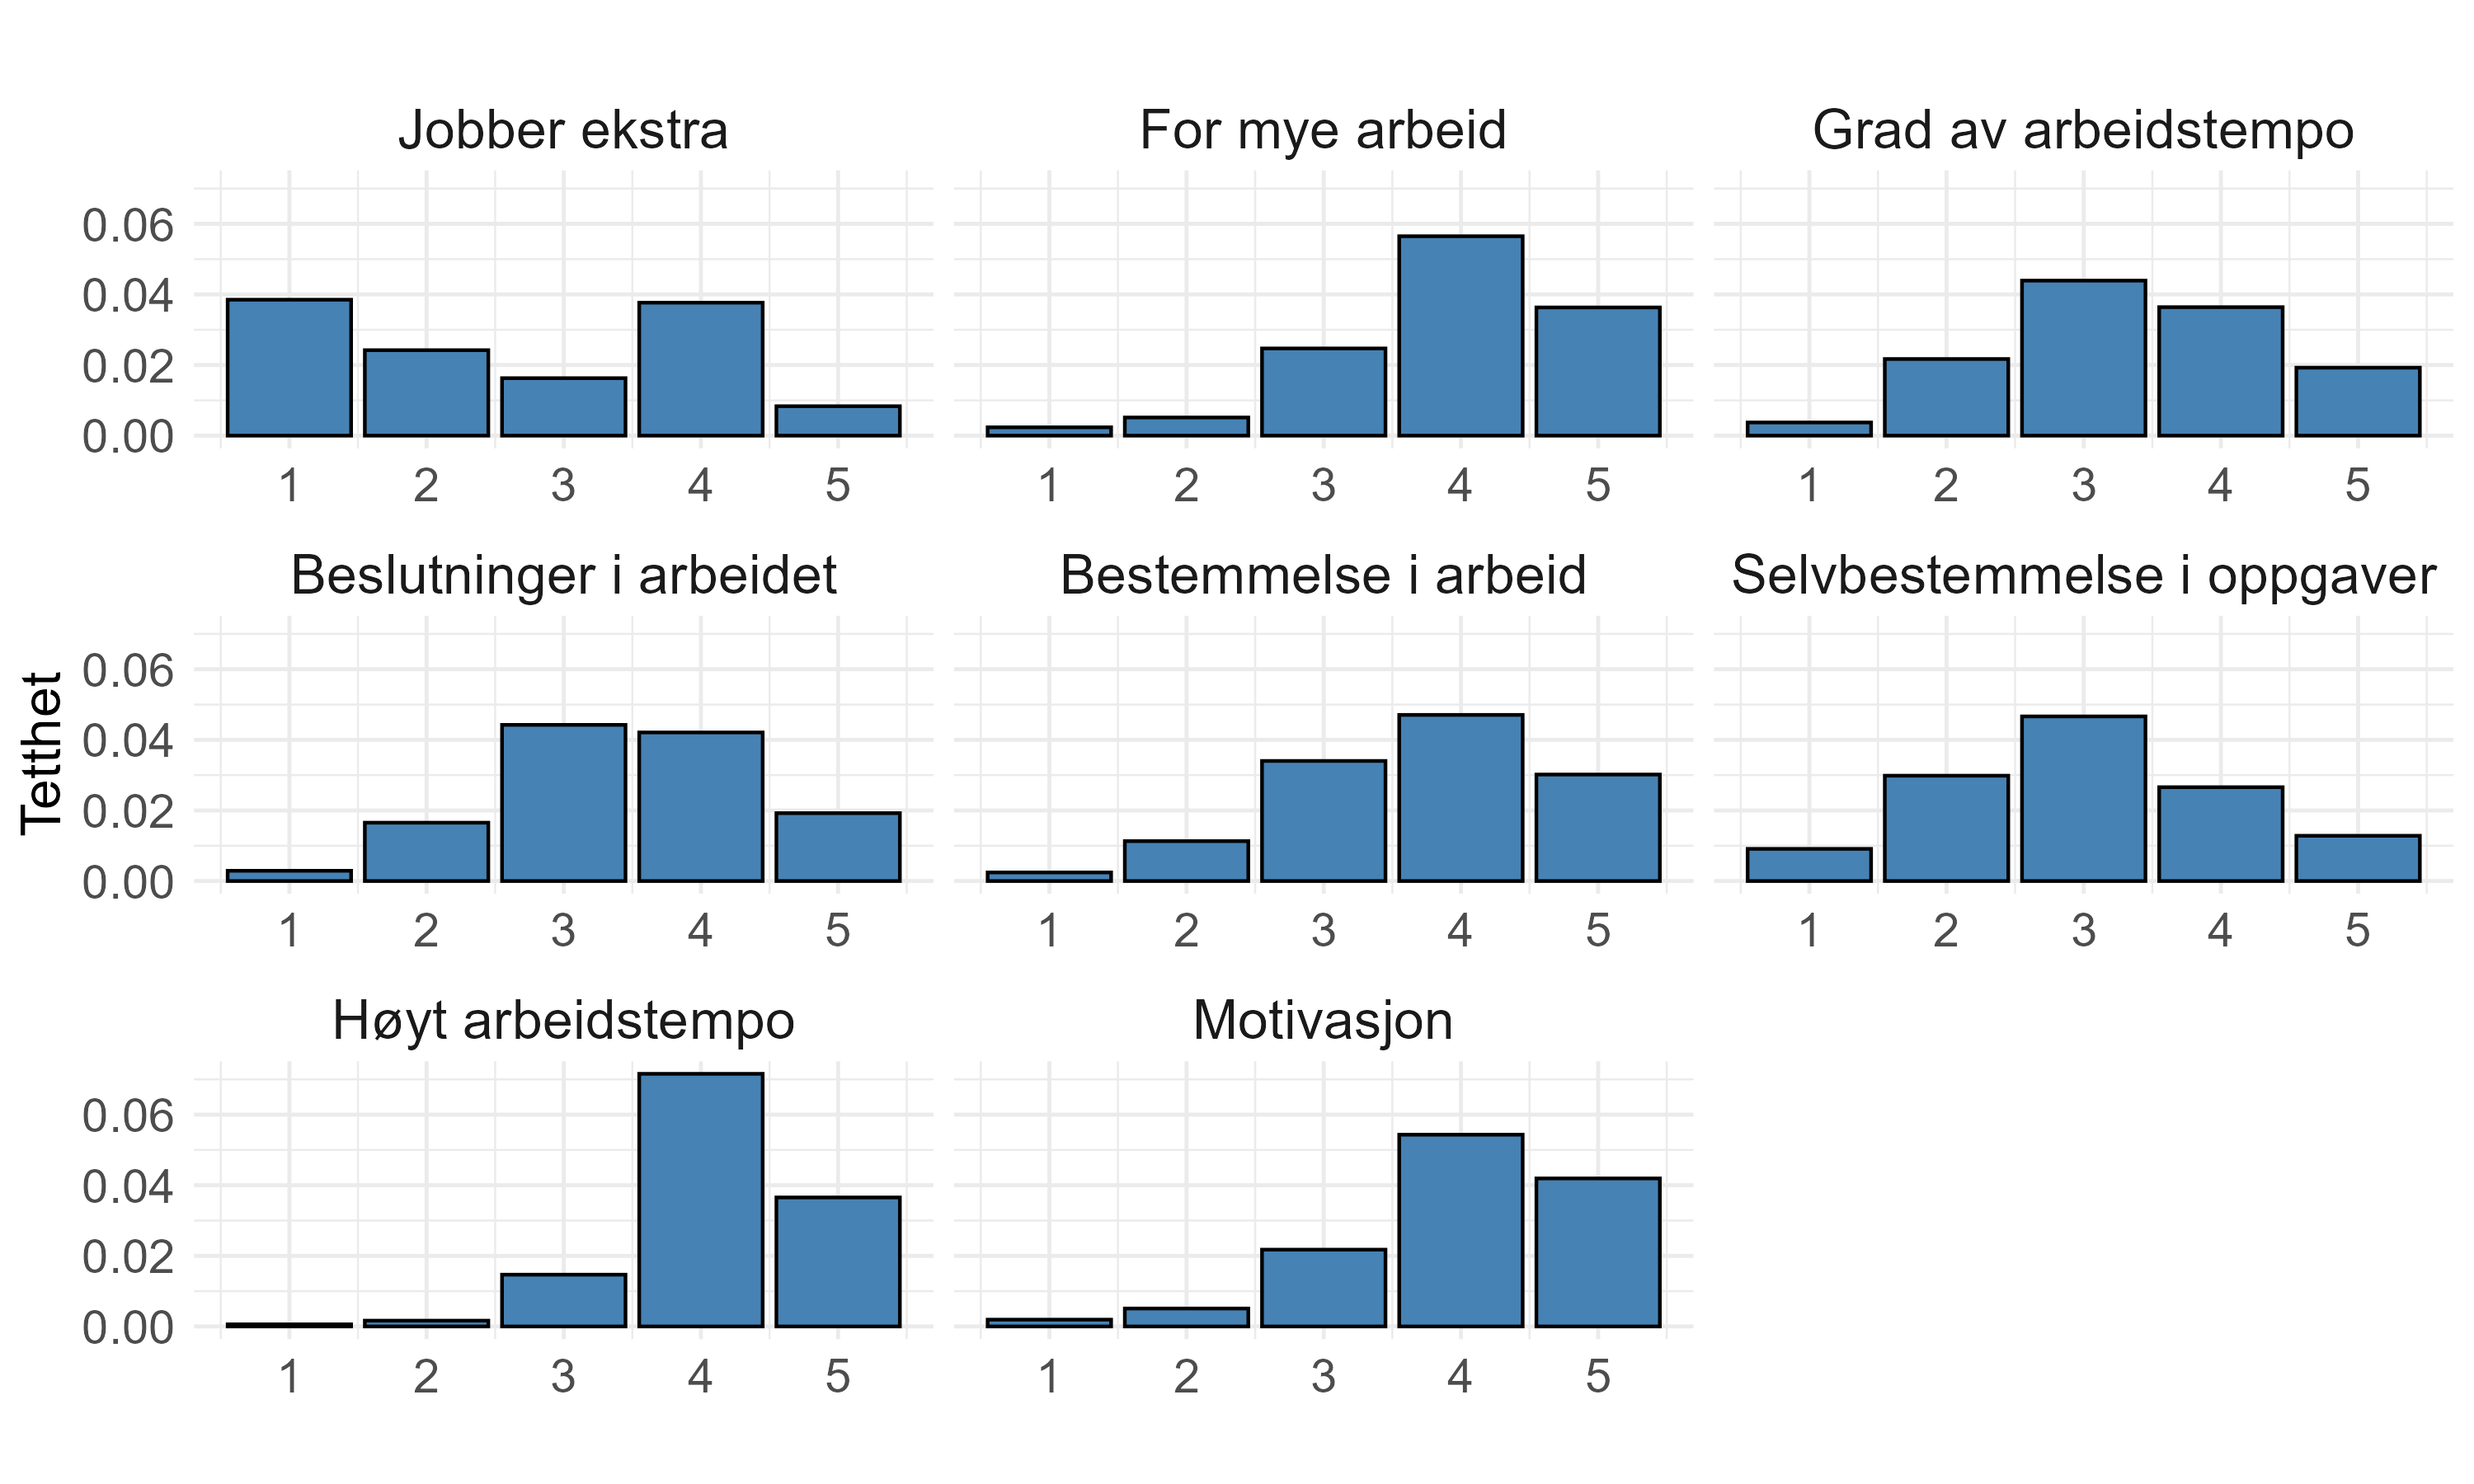
\includegraphics[width=0.8\textwidth]{dokumentobjekter/figurer/fig_kontrollvariabler.png}
\end{figure}
\vspace{-1cm}

\newpage

\section{Metode}\label{sec-metode}

\subsection{Structural Equation Model
(SEM)}\label{structural-equation-model-sem}

Vår analyse benytter en Structural Equation Model (SEM). Formue inngår
som en direkte forklaringsvariabel for både motivasjon og sykefravær.
Motivasjon modelleres som en medierende variabel, hvor jobbressurser og
formue kan påvirke motivasjonen, som igjen kan påvirke sykefraværet.
Jobbkrav antas å ha en direkte effekt på sykefravær.

Dette modellvalget bygger på JD-R-rammeverket. Ved å bruke en SEM-modell
kan vi teste de postulerte direkte og indirekte sammenhengene.

\subsubsection{Ligning til modellen}\label{ligning-til-modellen}

Modellen består av to ligninger: en for motivasjon (\(M_i\)) og en for
sykefravær (\(SF_i\)).

\paragraph{\texorpdfstring{Ligning for motivasjon
\(M_i\)}{Ligning for motivasjon M\_i}}\label{ligning-for-motivasjon-m_i}

Motivasjonen (\(M_i\)) antas å påvirkes av jobbressurser, formuenivå og
kontrollvariablene \(X_{ik}\).

\begin{equation}
  M_i = \alpha_0 + \alpha_1 JR_i + \alpha_2 FN_i + \sum_k \alpha_{3k}X_{ik} + \epsilon_{Mi} \label{eq:motivasjon}
\end{equation}

Hvor \(\alpha_0\) er konstantleddet, \(\alpha_1\) er effekten for
jobbressurser, \(\alpha_2\) er effekten av formue, og \(\alpha_{3k}\) er
effektene av kontrollvariablene. \(\epsilon_{Mi}\) er feilleddet for
motivasjonsmodellen.

\paragraph{\texorpdfstring{Hovedmodell for sykefravær
\(SF_i\)}{Hovedmodell for sykefravær SF\_i}}\label{hovedmodell-for-sykefravuxe6r-sf_i}

Sykefraværet antas å påvirkes direkte av jobbkrav (\(JK_i\)),
jobbressurser (\(JR_i\)), formue (\(FN_i\)) og motivasjon (\(M_i\)),
samt kontrollvariablene \(X_{ij}\).

\begin{equation}
SF_i = \beta_0 + \beta_1 JK_i + \beta_2 JR_i + \beta_3 FN_i
        + \beta_4 M_i + \Sigma_j \gamma_{j}X_{ij} + \epsilon_{1i} \label{eq:sf_utvidet}
\end{equation}

Hvor \(\beta_0\) er konstantleddet, \(\beta_1\) er effekten av jobbkrav,
\(\beta_2\) er effekten av jobbressurser, \(\beta_3\) er effekten av
formue, og \(\beta_4\) er effekten av motivasjon. \(\gamma_{j}\) er
effekten av kontrollvariablene \(X_{ij}\) som alder, stillingsprosent,
kjønn og utdanning. Dette vil si at for eksempel koeffisienten
\(\gamma_{SP}\) som del av \(\sum_j \gamma_{j}X_{ij}\) vil vise den
direkte sammenhengen mellom stillingsprosent og sykefravær kontrollert
for de andre variablene. \(\epsilon_{SFi}\) er feilleddet for
sykefraværmodellen.

\subsubsection{Forklaring av alle deler i
modellen}\label{forklaring-av-alle-deler-i-modellen}

\begin{table}[H]
\centering
\begin{tabular}{ll}
\toprule
Symbol & Forklaring \\ 
\midrule
$SF_i$ & Log-transformert sykefraværsprosent for individ $i$ \\
$JK_i$ & Latent variabel for individ $i$ (høyere = mer krav) \\
$JR_i$ & Latent variabel for individ $i$ (høyere = mer støtte/autonomi) \\
$FN_i$ & Normalisert formue (basert på qnorm-transformasjon) for individ $i$ \\
$M_i$ & Observert motivasjonsscore for individ $i$ \\
$X_{ik}/X_{ij}$ & Kontrollvariabler (for eks, alder, kjønn, utdanning, stillingsprosent),  \\
$\alpha_0, \beta_0$ & Konstantledd \\
$\alpha_1, \alpha_2, \beta_1, \beta_2, \beta_3, \beta_4$ & Strukturelle koeffisienter som estimerer styrken på sammenhengene \\
$\alpha_{3k}, \gamma_{j}$ & Koeffisienter for kontrollvariablene \\
$\epsilon_{Mi}, \epsilon_{SFi}$ & Feilledd for de endogene variablene motivasjon og sykefravær \\
\hline
\end{tabular}
\caption{Oversikt over variabler i modellen}
\label{tab:variabler}
\end{table}

\subsubsection{Beskrivning av metode}\label{beskrivning-av-metode}

Vår medierende variabel Motivasjon (\(M_i\)) i \autoref{eq:motivasjon}
er modellert som en funksjon av jobbressurser (\(JR_i\)) og formue
(\(FN_i\)), samt kontrollvariabler. Her forventer vi at \(\alpha_1 > 0\)
i tråd med JD-R modellen og Langseth-Eide \& Vittersø (2021) hvor
jobbressurser bygger engasjement og motivasjon. Vi forventer også at
\(\alpha_2 > 0\) som betyr at høyere formue vil føre til høyere
motivasjon. Dette bygger på antagelsen om at økonomisk trygghet
reduserer stress og frigjør mental kapasitet. Det bygger også på at på
at utsikter til økonomisk fremgang, eller fraværet av en følelse av at
det ikke er mulig å bli økonomisk trygg som kan oppstå ved stor ulikhet
Gesiarz et al. (2020), og at du dermed kan styrke den indre motivasjonen
for arbeidet.

\subsubsection{SEM-spesifikasjoner}\label{sem-spesifikasjoner}

Vi kjører to separate SEM-spesifikasjoner for å teste robustheten av
våre resultater. Den første inkluderer alle observasjoner i utvalget,
der sykefravær log-transformeres som log(sykefravær + 0.01) for å
håndtere nullverdier og skjevhet. Den andre modellen inkluderer kun
respondenter med registrert sykefravær, og benytter log(sykefravær
+0.01). Dette er for å undersøke om estimatene endres vesentlig når
null-gruppen utgår.

I appendix vil det være inkludert to tabeller der det er testet på
dataen for 2023 for å videre undersøke om det er noen endringer i
estimatene når vi bruker data fra 2023.

\paragraph{Endring av variabler}\label{endring-av-variabler}

De ordinale variablene har en skala fra 1-5, hvor 1 ofte er en form for
``oftest'' eller ``veldig fornøyd'', og 5 er ``aldri'' eller ``veldig
misfornøyd''.

Vi snur om på skalaen til de negative variablene fordi skalaen til
variabler som hvor fornøyd vil si at 1 er ofte veldig fornøyd, og 5
tilsier veldig misfornøyd, mens på foreks for mye å gjøre, så vil 1
tilsi daglig og 5 tilsi aldri. Som vi ser i \autoref{kontrollvariabler}
så vil det være enklere å tolke resultatene når vi har en skala som er
lik for alle variablene.

\subsubsection{Estimator}\label{estimator}

Siden flere av våre observerte variabler er ordinale, og fordi vi ikke
kan anta multivariat normalfordeling for alle variablene i modellen (se
foreks den markerte skjevheten for sykefravær i
\autoref{fig:histogram_sykefravar} og fordelingen av de ordinale
indikatorene i \autoref{fig:kontrollvariabler}), er estimatorer som
sannsynlighets maksimering ikke godt egnet. MLE forutsetter
kontinuerlige og multivariat normalfordelte data, og brudd på disse
antakelsene kan føre til upålitelige standardfeil og teststatistikker
(Finney \& DiStefano, 2006).

Gitt disse egenskapene ved våre data, har vi valgt å bruke
WLSMV-estimatoren (Weighted Least Squares Mean and Variance adjusted) i
vår SEM-analyse. WLSMV er en robust estimator som er spesielt utviklet
for modeller som inkluderer kategoriske eller ordinale observerte
variabler Muthén (1984). Den håndterer slike variabler ved å estimere en
matrise av polykoriske\footnote{Polykoriske korrelasjon beregner
  sammenhengen mellom to ordinale variabler ved å anta at hver av dem
  bunner i en latent, kontinuerlig fordeling} eller
polyseriale\footnote{Polyserial korrelasjon brukes når en variabel er
  ordinal og den andre er kontinuerlig. Det antas at den ordinale
  variabelen stammer fra en latent kontinuerlig skala, delt opp i
  kategorier av terskler.} korrelasjoner som input for analysen, sammen
med terskelverdier for de ordinale variablene. Disse tersklene
representerer de punktene på en underliggende kontinuerlig skala hvor
skillet mellom de observerte kategoriene går.

WLSMV estimatoren fungerer ved å minimere en veid sum av kvadrerte avvik
mellom de observerte og estimerte kovariansmatrisen. Betegnelsen MV
(Mean and Variance adjusted) i WLSMV indikerer at kji-kvadrat
teststørrelsen og standardfeilene er justert for å bedre håndtere avvik
fra antakelsen om multivariat normalfordeling. Justeringen gjøres ved
bruk av en diagonal vektmatrise som består består av variansene til de
estimerte korrelasjonene og tersklene.

I lavaan pakken har vi spesifisert parameteriseringen ``Theta'' som
modellerer feilvariansene til de latente responsvariablene som er under
de observerte ordinale variablene, og residualvariansene til de
observerte kontinuerlige variablene.

Variabelen for formue er transformert ved en invertert kumulativ
normalfordeling (Formue\_qnorm) for å håndtere dens skjevhet og for å
representere relativ formue. Sykefravær er log-transformert
(log(sykefravær+0.01)) i hovedmodellen (Modell 1) for å stabilisere
variansen og håndtere nullverdier. En alternativ modell (Modell 2)
benytter log(sykefravær + 0.01) på et subsett av data som ekskluderer
individer med null dager sykefravær for å teste robustheten til funnene.

\subsubsection{Hypoteser}\label{sec-hypot}

\paragraph{\texorpdfstring{Hypotese 1(H1): \(\beta_1 > 0\) Høyere
jobbkrav gir høyere
sykefravær}{Hypotese 1(H1): \textbackslash beta\_1 \textgreater{} 0 Høyere jobbkrav gir høyere sykefravær}}\label{hypotese-1h1-beta_1-0-huxf8yere-jobbkrav-gir-huxf8yere-sykefravuxe6r}

Dette er en grunnleggende antagelse i JD-R-modellen (Schaufeli \&
Bakker, 2004; Vander Elst et al., 2016). Høye krav (fysiske, psykiske,
emosjonelle) tærer på individets ressurser og kan føre til utbrenthet og
helseplager, som igjen øker sannsynligheten for sykefravær.

\paragraph{\texorpdfstring{Hypotese 2(H2): \(\beta_2 < 0\) Høyere
jobbressurser gir lavere
sykefravær}{Hypotese 2(H2): \textbackslash beta\_2 \textless{} 0 Høyere jobbressurser gir lavere sykefravær}}\label{hypotese-2h2-beta_2-0-huxf8yere-jobbressurser-gir-lavere-sykefravuxe6r}

Jobbressurser (støtte, autonomi, tilbakemelding) fungerer som
beskyttende faktorer. De hjelper ansatte med å håndtere krav, oppnå mål
og fremmer personlig vekst, noe som fører til høyere engasjement og
bedre helse, og dermed lavere fravær (Langseth-Eide \& Vittersø, 2021).

\paragraph{\texorpdfstring{Hypotese 3(H3): \(\beta_3 < 0\) Høyere
formuenivå gir lavere
sykefravær}{Hypotese 3(H3): \textbackslash beta\_3 \textless{} 0 Høyere formuenivå gir lavere sykefravær}}\label{hypotese-3h3-beta_3-0-huxf8yere-formuenivuxe5-gir-lavere-sykefravuxe6r}

Vi forventer en direkte, gunstig effekt av formue på sykefravær. Formue
fungerer som en ``buffer'' mot levekårsproblemer (Hattrem, n.d.;
Normann, 2009) og gir økonomisk trygghet. Dette kan redusere generelt
stressnivå og forbedre helsen, slik funn fra Jaeggi et al. (2021)
indikerer (høyere formue -\textgreater{} lavere blodtrykk, færre
luftveissykdommer). Økonomisk trygghet kan også gi bedre tilgang til
helsetjenester og en større evne til å håndtere helseutfordringer uten å
måtte ty til langvarig fravær.

\paragraph{\texorpdfstring{Hypotese 4(H4): Formue øker motivasjon
\(\alpha_2 > 0\)}{Hypotese 4(H4): Formue øker motivasjon \textbackslash alpha\_2 \textgreater{} 0}}\label{hypotese-4h4-formue-uxf8ker-motivasjon-alpha_2-0}

Vi forventer en indirekte vei der formue påvirker sykefravær gjennom
motivasjon. Som nevnt \autoref{sec-formue-jdr}, forventer vi at høyere
formue øker motivasjonen \(\alpha_2 > 0\) som ved å redusere finansiell
usikkerhet, og gode fremtidsutsikter. Videre forventer vi at høyere
motivasjon/engasjement reduserer sykefraværet, slik Langseth-Eide \&
Vittersø (2021) fant.

\newpage

\section{Analyse og resultater}\label{sec-analyse}

I dette kapittelet presenter vi resultatene fra SEM-analysen. Analysen
er utført med lavaan-pakken i R, basert på den teoretiske modellen og
metodebeskrivelsen i henholdsvis kapittel \ref{sec:teori} og
\ref{sec-metode}. Formålet er å undersøke sammenhengen mellom formue,
jobbkrav, jobbressurser, motivasjon og sykefravær. Vi benytter en
Weighted Least Squares Mean and Variance adjusted (WLSMV) estimator.
Denne estimatoren er valgt fordi flere av våre sentrale
indikatorvariabler (som måler jobbkrav, jobbressurser og motivasjon) er
ordinale, og fordi vi ikke kan anta normalfordeling for alle variablene
som vist i \autoref{fig:kontrollvariabler}, spesielt ikke for sykefravær
som vist i \autoref{fig:histogram_sykefravar_log}.

Resultatene presenteres i to modeller: Modell 1 inkluderer alle
respondenter hvor sykefravær er log-transformert (logsyk =
\(log(sykefravær_2022+0.01)\)), mens Modell 2 kun inkluderer
respondenter med registrert sykefravær og benytter samme
log-transformasjon (logsyk\_u0 = \(log(sykefravær_2022+0.01)\)). Dette
gjøres for å kunne sjekke om resultatene er robuste når vi ekskluderer
individer med null sykefravær. Vi presenterer også resultater for 2023 i
appendix for å undersøke om det er noen endringer i estimatene når vi
bruker data fra 2023.

\subsubsection{Tolkning av resultater}\label{tolkning-av-resultater}

Tolkning av resultat-tabellene

Resultatene fra SEM-analysene presenteres i tabellform

Avhengig variabel: Viser hvilken endogen variabel i modellen som
predikeres i den aktuelle delen av tabellen (enten Motivasjon eller
logsyk/logsyk\_u0).

Prediktor: Navnet på den uavhengige variabelen (observert eller latent)
eller kontrollvariabelen som predikerer den avhengige variabelen.
Bokstavkombinasjonene i parentes (f.eks. \(\alpha_1\), \(\beta_1\))
refererer til parameterbenevnelsene brukt i våre ligningsspesifikasjoner
i kapittel \ref{sec-metode} og i lavaan-koden.

Estimat: Dette er den ustandardiserte regresjonskoeffisienten. Den viser
endringen i den avhengige variabelen for en enhets endring i
prediktorvariabelen, kontrollert for alle andre variabler i ligningen.
For eksempel, hvis logsyk er avhengig variabel og Formue\_qnorm er
prediktor, viser estimatet hvor mye logsyk endres når Formue\_qnorm øker
med én enhet (som tilsvarer ett standardavvik i den normaliserte
formuesfordelingen).

Std.Err: Standardfeilen til estimatet. Dette er et mål på usikkerheten i
estimatet; mindre standardfeil indikerer større presisjon.

z-verdi: Teststørrelsen for koeffisienten, beregnet som
\(\frac{\text{Estimat}}{\text{Std.Err}}\). Den brukes til å vurdere om
koeffisienten er signifikant forskjellig fra null.

p-verdi: Sannsynligheten for å observere en z-verdi som er minst like
ekstrem som den beregnede, gitt at nullhypotesen (om at den sanne
koeffisienten er null) er sann. Vi benevner p-verdier som signifikante
hvis de er mindre enn 0.05, og svært signifikante hvis de er mindre enn
0.001.

Std.all: Den fullstendig standardiserte koeffisienten. Denne
koeffisienten indikerer hvor mange standardavvik den avhengige
variabelen endres med når den uavhengige variabelen endres med ett
standardavvik, kontrollert for andre variabler. Dette gjør det lettere å
sammenligne styrken på effekter mellom ulike prediktorer som er målt på
forskjellige skalaer.

\subsubsection{Resultat for vår
hovedmodell}\label{resultat-for-vuxe5r-hovedmodell}

\begin{table}[htbp]
\centering
\caption{Resultater fra strukturmodellen (Modell 1) for prediksjon av motivasjon og sykefravær (\texttt{logsyk}).}
\label{tab:sem_results_model1}
\begin{tabular}{@{}llrrrrc@{}}
\toprule
Avhengig variabel & Prediktor & Estimat & Std.Err & z-verdi & p-verdi & Std.all \\
\midrule
\multicolumn{7}{l}{\textit{Prediktorer for motivasjon}} \\
& \texttt{Latent\_JR} ($\alpha_1$) & 0.479 & 0.019 & 25.304 & <0.001 & 0.430 \\
& \texttt{Formue\_qnorm} ($\alpha_2$) & 0.008 & 0.017 & 0.479 & 0.632 & 0.007 \\
& \texttt{ald\_ung} (c1) & -0.363 & 0.045 & -8.098 & <0.001 & -0.121 \\
& \texttt{ald\_elder} (c2) & 0.253 & 0.041 & 6.192 & <0.001 & 0.093 \\
& \texttt{Kvinne} (c3) & 0.013 & 0.033 & 0.406 & 0.685 & 0.006 \\
& \texttt{Utd\_grunnskole} (c4) & 0.016 & 0.047 & 0.346 & 0.730 & 0.005 \\
& \texttt{Utd\_universitet} (c5) & -0.016 & 0.035 & -0.462 & 0.644 & -0.007 \\
& \texttt{Barn} (c6) & 0.017 & 0.046 & 0.379 & 0.704 & 0.005 \\
& \texttt{arb\_stillingspst} (c7) & 0.004 & 0.001 & 6.134 & <0.001 & 0.087 \\
\midrule
\multicolumn{7}{l}{\textit{Prediktorer for sykefravær (\texttt{logsyk})}} \\
& \texttt{Latent\_JK} ($\beta_1$) & 0.042 & 0.020 & 2.071 & 0.038 & 0.035 \\
& \texttt{Latent\_JR} ($\beta_2$) & -0.087 & 0.013 & -6.887 & <0.001 & -0.108 \\
& \texttt{Formue\_qnorm} ($\beta_3$) & -0.104 & 0.012 & -9.015 & <0.001 & -0.123 \\
& \texttt{Motivasjon} ($\beta_4$) & -0.033 & 0.011 & -2.951 & 0.003 & -0.046 \\
& \texttt{ald\_ung} ($\gamma_1$) & 0.010 & 0.029 & 0.344 & 0.731 & 0.005 \\
& \texttt{ald\_elder} ($\gamma_2$) & 0.005 & 0.026 & 0.191 & 0.848 & 0.003 \\
& \texttt{Kvinne} $\gamma_3$ & 0.216 & 0.022 & 9.674 & <0.001 & 0.130 \\
& \texttt{Utd\_grunnskole} $\gamma_4$ & 0.037 & 0.030 & 1.230 & 0.219 & 0.015 \\
& \texttt{Utd\_universitet} $\gamma_5$ & -0.113 & 0.024 & -4.709 & <0.001 & -0.066 \\
& \texttt{Barn} $\gamma_6$ & 0.042 & 0.030 & 1.411 & 0.158 & 0.018 \\
& \texttt{arb\_stillingspst} $\gamma_7$ & 0.002 & 0.000 & 3.356 & 0.001 & 0.045 \\
\bottomrule
\end{tabular}
\raggedright
\footnotesize{\textit{Merk:} Estimat er ustandardisert koeffisient. Std.Err er standardfeil. Std.all er fullstendig standardisert koeffisient. Referansekategorier: Alder (30–54 år), Utdanning (videregående). \texttt{Formue\_qnorm} er normalisert formue. \texttt{arb\_stillingspst} er stillingsprosent. \texttt{logsyk} er log(sykefravær + 0.01).}
\end{table}

\subsection{Resultat knyttet til modell
1}\label{resultat-knyttet-til-modell-1}

\subsubsection{Prediksjon av log-transformert sykefravær i modell
1.}\label{prediksjon-av-log-transformert-sykefravuxe6r-i-modell-1.}

\paragraph{\texorpdfstring{Hypotese 1 Jobbkrav
\(\text{Latent JK} \rightarrow \text{Sykefravær } \beta_1 > 0\)}{Hypotese 1 Jobbkrav \textbackslash text\{Latent JK\} \textbackslash rightarrow \textbackslash text\{Sykefravær \} \textbackslash beta\_1 \textgreater{} 0}}\label{hypotese-1-jobbkrav-textlatent-jk-rightarrow-textsykefravuxe6r-beta_1-0}

Vi finner en positiv og statistisk signifikant sammenheng mellom
\textbf{Jobbkrav (\texttt{Latent\_JK})} og \texttt{logsyk} (Estimat =
\(0.042\), Std.all = \(0.035\), \(p = 0.038\)). Dette gir støtte til H1.
Økte jobbkrav er assosiert med en økning i log-transformert sykefravær.
Effekten er relativt liten, men signifikant, som indikerer at høyere
opplevde krav i jobben er forbundet med høyere sykefravær.

\paragraph{\texorpdfstring{Hypotese 2
\(\text{Latent JR} \rightarrow \text{Sykefravær } \beta_2 < 0\)}{Hypotese 2 \textbackslash text\{Latent JR\} \textbackslash rightarrow \textbackslash text\{Sykefravær \} \textbackslash beta\_2 \textless{} 0}}\label{hypotese-2-textlatent-jr-rightarrow-textsykefravuxe6r-beta_2-0}

Det er en negativ og statistisk signifikant sammenheng mellom
Jobbressurser (Latent\_JR) og logsyk (Estimat = \(-0.087\), Std.all =
\(-0.108\), \(p < 0.001\)). Dette gir i utgangspunktet sterk støtte til
H2. Økt tilgang på jobbressurser er assosiert med en reduksjon i
log-transformert sykefravær.

\paragraph{\texorpdfstring{Hypotese 3
\(\text{Formue} \rightarrow \text{Sykefravær } \beta_3 < 0\)}{Hypotese 3 \textbackslash text\{Formue\} \textbackslash rightarrow \textbackslash text\{Sykefravær \} \textbackslash beta\_3 \textless{} 0}}\label{hypotese-3-textformue-rightarrow-textsykefravuxe6r-beta_3-0}

Formue (Formue\_qnorm) viser en negativ og statistisk signifikant
sammenheng med logsyk (Estimat = \(-0.104\), Std.all = \(-0.123\),
\(p < 0.001\)). Dette gir sterk støtte til H3. En økning på et
standardavvik i den normaliserte formueskalaen har en reduksjon på 0.104
i log-transformert sykefravær, selv når vi kontrollerer for jobbkrav,
jobbressurser og motivasjon.

\subsubsection{Prediksjon av motivasjon}\label{prediksjon-av-motivasjon}

\paragraph{Hypotese 4}\label{hypotese-4}

Som vist i øvre del av \autoref{tab:sem_results_model1}, er
Jobbressurser (Latent\_JR) en sterk og positiv prediktor for Motivasjon
(Estimat = \(0.479\), Std.all = \(0.430\), \(p < 0.001\)). Dette er i
tråd med JD-R-modellen, som postulerer at ressurser i jobben fremmer en
motiverende prosess. Formue (Formue\_qnorm) viser derimot ingen
signifikant direkte sammenheng med Motivasjon (Estimat = \(0.008\),
\(p = 0.632\)). Vår antakelse om at formue direkte påvirker motivasjon
får dermed ikke støtte i denne modellen.

\subsubsection{Redegjørelse for effekt av kontrollvariabler i modell
1.}\label{redegjuxf8relse-for-effekt-av-kontrollvariabler-i-modell-1.}

\paragraph{Sykefravær}\label{sykefravuxe6r-1}

Kvinner har signifikant høyere sykefravær enn menn (Estimat = 0.216,
Std.all = 0.130, p\textless0.001).

Universitetsutdanning er assosiert med signifikant lavere sykefravær
(Estimat = −0.113, Std.all = −0.066, p\textless0.001) sammenlignet med
de med videregående utdanning. Grunnskoleutdanning viser ingen
signifikant forskjell fra videregående.

Høyere stillingsprosent gir signifikant resultat på høyere sykefravær
(Estimat = 0.002, Std.all = 0.045, p=0.001). Resultatet her tilsier at å
har stilling over gjennomsnittet er knyttet til noe høyere fravær.

Aldersgruppene viser ingen signifikant forskjell i sykefravær fra
referansegruppen (30-54 år), og heller ikke om de har barn under 5 år
viser noe signifikant effekt.

\paragraph{Motivasjon}\label{motivasjon-1}

Unge arbeidstakere (ald\_ung, 18-29 år) rapporterer signifikant lavere
motivasjon (Estimat = −0.363, Std.all = −0.121, p\textless0.001) enn
referansegruppen (30-54 år).

Eldre arbeidstakere (ald\_elder, 55-66 år) rapporterer signifikant
høyere motivasjon (Estimat = 0.253, Std.all = 0.093, p\textless0.001)
enn referansegruppen.

Høyere stillingsprosent (arb\_stillingspst) er også assosiert med
signifikant høyere sykefravær (Estimat = 0.004, Std.all = 0.087,
p\textless0.001).

Kjønn, utdanningsnivå og om individet har barn under 5 år viser ingen
signifikant sammenheng med motivasjon i denne modellen.

\subsection{Resultat knyttet til modell
2}\label{resultat-knyttet-til-modell-2}

Siden sykefraværet er så høyreskjevt selv når det er log-transformert i
\autoref{fig:histogram_sykefravar}, kan det gi oss p-verdier som er for
lave, og dermed kan det være at vi overestimerer effekten av
prediktorene.

Hvis vi ekskluderer de uten legemeldt sykefravær og log-transformerer
sykefraværet uten å legge til 0.01, slik at det er tilnærmet
normalfordelt, så kan vi se om dette endrer resultatene. Dette er gjort
i modell 2, og vi ser at det er store endringer i resultatene.

\begin{table}[htbp]
\centering
\caption{SEM‐resultater (Modell 2): Prediksjon av motivasjon og sykefravær (\texttt{logsyk\_u0}), estimert kun på de med sykefravær < 0 ($N = 2021$).}
\label{tab:sem_results_model2}
\begin{tabular}{@{}llrrrrc@{}}
\toprule
Avhengig variabel & Prediktor & Estimat & Std.Err & z‐verdi & p‐verdi & Std.all \\
\midrule
\multicolumn{7}{l}{\textit{Prediktorer for \texttt{Motivasjon}}} \\
& \texttt{Latent\_JR} ($\alpha_1$)        & 0.548 & 0.038 & 14.610 & <0.001 & 0.431 \\
& \texttt{Formue\_qnorm} ($\alpha_2$)     & 0.022 & 0.030 & 0.742  & 0.458  & 0.018 \\
& \texttt{ald\_ung} (c1)          & -0.463& 0.075 & -6.206 & <0.001 & -0.161 \\
& \texttt{ald\_elder} (c2)        & 0.183 & 0.073 & 2.524  & 0.012  & 0.065 \\
& \texttt{Kvinne} (c3)            & 0.132 & 0.058 & 2.291  & 0.022  & 0.057 \\
& \texttt{Utd\_grunnskole} (c4)   & 0.052 & 0.076 & 0.685  & 0.493  & 0.016 \\
& \texttt{Utd\_universitet} (c5)  & -0.146& 0.064 & -2.273 & 0.023  & -0.061 \\
& \texttt{Barn} (c6)              & 0.068 & 0.078 & 0.873  & 0.383  & 0.021 \\
& \texttt{arb\_stillingspst} (c7) & 0.001 & 0.001 & 1.079  & 0.281  & 0.027 \\
\midrule
\multicolumn{7}{l}{\textit{Prediktorer for \texttt{logsyk\_u0}}} \\
& \texttt{Latent\_JK} ($\beta_1$)        & 0.027 & 0.024 & 1.151  & 0.250  & 0.034 \\
& \texttt{Latent\_JR} ($\beta_2$)        & -0.030& 0.022 & -1.347 & 0.178  & -0.039 \\
& \texttt{Formue\_qnorm} ($\beta_3$)     & -0.075& 0.018 & -4.304 & <0.001 & -0.102 \\
& \texttt{Motivasjon} ($\beta_4$)        & -0.040& 0.017 & -2.389 & 0.017  & -0.067 \\
& \texttt{ald\_ung} ($\gamma_1$)          & -0.078& 0.042 & -1.859 & 0.063  & -0.045 \\
& \texttt{ald\_elder} ($\gamma_2$)        & 0.124 & 0.040 & 3.092  & 0.002  & 0.073 \\
& \texttt{Kvinne} $\gamma_3$            & 0.056 & 0.032 & 1.725  & 0.085  & 0.040 \\
& \texttt{Utd\_grunnskole} $\gamma_4$   & -0.001& 0.044 & -0.016 & 0.987  & -0.000 \\
& \texttt{Utd\_universitet} $\gamma_5$  & -0.044& 0.035 & -1.231 & 0.218  & -0.030 \\
& \texttt{Barn} $\gamma_6$              & 0.035 & 0.042 & 0.837  & 0.403  & 0.018 \\
& \texttt{arb\_stillingspst} $\gamma_7$ & -0.002& 0.001 & -2.363 & 0.018  & -0.051 \\
\bottomrule
\end{tabular}
\raggedright
\footnotesize{%
\textit{Merk:} Alle estimeringer er gjort på subutvalget av respondenter med sykefravær < 0 (N = 2021). Estimat = ustandardisert koeffisient; Std.Err = robust standardfeil; z-verdi = z-teststatistikk; p-verdi = sannsynlighet for z-verdien; Std.all = fullstendig standardisert koeffisient. Referansekategorier: Alder (30–54 år), Utdanning (videregående). \texttt{arb\_stlln} er arbeidsstillingsprosent}
\end{table}

\subsection{Resultat knyttet til modell
2}\label{resultat-knyttet-til-modell-2-1}

Det er langt mye færre signifikante resultater i modell 2 enn i modell
1, og det er også en del endringer i retning på effektene. Dette kan
indikere at de som ikke har sykefravær har en annen sammenheng mellom
jobbkrav, jobbressurser, formue og sykefravær enn de som har sykefravær,
eller at p-verdiene i modell 1 er for lave på grunn av skjevheten i
sykefraværsdataene. Vi vil derfor tolke resultatene med forsiktighet, og
vi vil også diskutere svakhetene i modellen og dataene i kapittel
\ref{sec-diskusjon}.

\subsubsection{Prediksjon av log-transformert sykefravær i modell
2.}\label{prediksjon-av-log-transformert-sykefravuxe6r-i-modell-2.}

\paragraph{\texorpdfstring{Hypotese 1 Jobbkrav
\(\text{Latent JK} \rightarrow \text{Sykefravær } \beta_1 > 0\)}{Hypotese 1 Jobbkrav \textbackslash text\{Latent JK\} \textbackslash rightarrow \textbackslash text\{Sykefravær \} \textbackslash beta\_1 \textgreater{} 0}}\label{hypotese-1-jobbkrav-textlatent-jk-rightarrow-textsykefravuxe6r-beta_1-0-1}

Effekten er ikke signifikant (Estimat = \(0.027\), Std.all = \(0.034\),
\(p = 0.250\)). Dette indikerer at jobbkrav ikke har en signifikant
direkte effekt på sykefravær blandt de som hadde mer enn 0 dager
sykefravær i 2022. Støtten for H1 svekkes og vi kan ikke med sikkerhet
si at høyere jobbkrav er assosiert med høyere sykefravær i denne
undergruppen av respondenter.

\paragraph{\texorpdfstring{Hypotese 2
\(\text{Latent JR} \rightarrow \text{Sykefravær } \beta_2 < 0\)}{Hypotese 2 \textbackslash text\{Latent JR\} \textbackslash rightarrow \textbackslash text\{Sykefravær \} \textbackslash beta\_2 \textless{} 0}}\label{hypotese-2-textlatent-jr-rightarrow-textsykefravuxe6r-beta_2-0-1}

Effekten er negativ men ikke signifikant (Estimat = \(-0.030\), Std.all
= \(-0.039\), \(p = 0.178\)). Dette indikerer at jobbressurser ikke har
en signifikant direkte effekt på sykefravær blant de som hadde mer enn 0
dager sykefravær i 2022. Støtten for H2 svekkes også.

\paragraph{\texorpdfstring{Hypotese 3
\(\text{Formue} \rightarrow \text{Sykefravær } \beta_3 < 0\)}{Hypotese 3 \textbackslash text\{Formue\} \textbackslash rightarrow \textbackslash text\{Sykefravær \} \textbackslash beta\_3 \textless{} 0}}\label{hypotese-3-textformue-rightarrow-textsykefravuxe6r-beta_3-0-1}

Formue (Formue\_qnorm) har en signifikant negativ effekt på sykefravær
(Estimat = \(-0.075\), Std.all = \(-0.102\), \(p < 0.001\)). Dette
styrker H3. En økning på et standardavvik i den normaliserte
formueskalaen er assosiert med en reduksjon i log-transformert
sykefravær, selv når vi kun ser på de som har sykefravær. Dette
indikerer at formue fortsatt fungerer som en buffer mot sykefravær i
denne undergruppen av respondenter.

\subsubsection{Prediksjon av
motivasjon}\label{prediksjon-av-motivasjon-1}

\paragraph{Hypotese 4}\label{hypotese-4-1}

Motivasjon er fortsatt negativt og signifikant assosiert med sykefravær
(Estimat = \(-0.040\), Std.all = \(-0.067\), \(p = 0.017\)). Dette
styrker H4.

Formue ser ikke ut til å ha noe signifikant direkte effekt på motivasjon
i denne modellen (Estimat = \(0.022\), \(p = 0.458\)).

\subsubsection{Redegjørelse for effekt av kontrollvariabler i modell
2.}\label{redegjuxf8relse-for-effekt-av-kontrollvariabler-i-modell-2.}

\paragraph{Sykefravær}\label{sykefravuxe6r-2}

Eldre arbeidstakere (ald\_elder, 55-66 år) rapporterer signifikant
høyere sykefravær (Estimat = 0.124, Std.all = 0.073, \(p = 0.002\)) enn
referansegruppen (30-54 år). Dette var ikke fanget opp i modell 1.

Stillingsprosenten snur retning og blir negativt assosiert med
sykefravær (Estimat = \(-0.002\), Std.all = \(-0.051\), \(p = 0.018\)).
Dette indikerer at høyere stillingsprosent er assosiert med lavere
sykefravær i denne undergruppen av respondenter. Dette kan tilsi at av
de som har sykefravær så er det de med lavere stillingsprosent som har
høyere sykefravær, mens de med høyere stillingsprosent har lavere
sykefravær. Effektstørrelsen i begge retninger er imidlertid liten.

Kjønn er ikke lengere signifikant assosiert med sykefravær (Estimat =
0.056, Std.all = 0.040, \(p = 0.085\)), noe som kan indikere at
forskjellene i sykefravær mellom kjønnene er mindre når vi kun ser på de
med sykefravær og at det er skjevheten i sykefraværsdataene som har
gjort at det så ut til å være en signifikant forskjell i modell 1.

Utdanningsnivå viser ingen signifikant effekt på sykefravær i denne
modellen.

\paragraph{Motivasjon}\label{motivasjon-2}

Laten variabelen Jobbressurser (Latent\_JR) er fortsatt en sterk og
positiv prediktor for Motivasjon (Estimat = \(0.548\), Std.all =
\(0.431\), \(p < 0.001\)). Dette styrker funnet i modell 1 og gir
fortsatt støtte til JD-R-modellen.

Formue har ingen signifikant effekt på Motivasjon.

I modell 2 blir har nå kjønn en signifikant positiv effekt på motivasjon
(Estimat = 0.132, Std.all = 0.057, \(p = 0.022\)). Dette indikerer at
kvinner rapporterer høyere motivasjon enn menn, og utdanningsnivået
universitetsutdanning er fortsatt assosiert med lavere motivasjon
(Estimat = \(-0.146\), Std.all = \(-0.061\), \(p = 0.023\)) sammenlignet
med de med videregående utdanning.

Stillingsprosent er ikke lenger signifikant assosiert med motivasjon
(Estimat = \(0.001\), Std.all = \(0.027\), \(p = 0.281\)).

\subsection{Sammenligning av modell 1 og modell
2}\label{sammenligning-av-modell-1-og-modell-2}

Modell 1 inkluderer alle respondenter, mens modell 2 kun inkluderer de
med registrert sykefravær. Dette kan påvirke resultatene, spesielt for
sykefravær, da modell 1 kan ha skjevheter på grunn av nullverdier i
sykefravær. Modell 2 gir en mer presis vurdering av sammenhengene blant
de som faktisk har sykefravær. Det er en del motsetninger i resultatene
mellom modell 1 og modell 2 noe som svekker troverdigheten til
hypotesene.

Hovedforskjellen er at effektene til jobbkrav og jobbressurser på
sykefravær mister sin signifikans i modell 2, noe som kan indikere at
disse sammenhengene er mindre robuste eller muligens ikke lineære. Dette
kan skyldes at de som har sykefravær har en annen dynamikk enn de som
ikke har det, eller at skjevheten i sykefraværsdataene i modell 1 har
påvirket resultatene.

Formue og motivasjon beholder derimot en signifikant negativ effekt på
sykefravær i begge modeller, noe som styrker hypotesen om at formue
fungerer som en buffer mot sykefravær.

\subsection{Modeltilpasning}\label{modeltilpasning}

\begin{table}[htbp]
\centering
\caption{Sammenligning av Fit-Indekser for Modell 1 og Modell 2}
\label{tab:fit_comparison_model1_model2}
\begin{tabular}{@{}lcc@{}}
\toprule
Fit Indeks                      & Modell 1 (N=6103) & Modell 2 (N=2021) \\
\midrule
Chi-kvadrat (Skalert test)      & 1470.660          & 432.960           \\
Frihetsgrader (df)              & 80                & 80                \\
P-verdi (Chi-kvadrat)           & < 0.001           & < 0.001           \\
CFI (Skalert)                   & 0.932             & 0.941             \\
TLI (Skalert)                   & 0.969             & 0.973             \\
RMSEA (Skalert)                 & 0.053             & 0.047             \\
RMSEA 90\% KI                   & [0.051, 0.056]    & [0.042, 0.051]    \\
P-verdi (RMSEA $\le$ 0.050)     & 0.010             & 0.889             \\
SRMR                            & 0.035             & 0.040             \\
\bottomrule
\end{tabular}
\raggedright
\footnotesize{%
\textit{Merk:} KI = Konfidensintervall.
}
\end{table}

For begge modeller er \(\chi^2\)-verdien signifikant som indikerer en
signifikant forskjell mellom observert og estimert kovariansmatrise. Men
siden \(\chi^2\)-testen er sensitiv for store utvalg så kan dette
fremdeles godkjennes.

Comparative Fit Index (CFI) og Tucker-Lewis Index (TLI) er begge over
0.90, noe indikerer god tilpasning for begge modeller. Root Mean Square
Error of Approximation (RMSEA) er under 0.06 for begge modeller, noe som
også indikerer god tilpasning. Standardized Root Mean Square Residual
(SRMR) er under 0.08 for begge modeller, noe som også er et tegn på god
tilpasning.

\subsubsection{Redegjørelse for svakheter i
modellen/data}\label{redegjuxf8relse-for-svakheter-i-modellendata}

Til å starte med så er denne typen modell i grensepunktet på vår
forståelse og dette fører til at det må tilføyes usikkerhet til
tolkningen av resultatene. Spesielt gjelder dette for forståelsen av
modelltilpasning, estimatorjusteringer og tolkning av latente
sammenhenger i strukturelle ligningsmodeller med kategoriske data. Selv
om analysen bygger på anerkjent metode og teori, er SEM med latente
variabler og robuste estimatorer som WLSMV et metodisk nivå som ligger i
ytterkanten av hva vi på bachelor nivå kan tolke. Resultatene diskuteres
derfor med forsiktighet, og vi legger vekt på overordnede mønstre
fremfor detaljerte tolkninger.

Vi har ikke testet med egenmeldt sykefravær da dette var en ja/nei
kategori i datasettet.

\newpage

\section{Diskusjon}\label{diskusjon}

\paragraph{får se om vi beholder
dette}\label{fuxe5r-se-om-vi-beholder-dette}

Karrierevalg og utdanning fra gallup som viste en fattigere har
dårligere tilgang på ``career role models'' som gjør at de kanskje ikke
vet om de bedre yrkene og sånt og dermed igjen blir mindre utdanna og
sånt https://www.gallup.com/analytics/506696/amazon-research-hub.aspx så
effekt på karriærevalg, utdanning osv. langsiktig effekt av
formue/bakrunn er noe påvirker hvilken type jobb folk har og dermed
jobbkrav og jobbresssurser. Dette er da en indirekte effekt som vi ikke
får med.

\subsubsection{Formueeffekt på konsum}\label{formueeffekt-puxe5-konsum}

https://fnce.wharton.upenn.edu/wp-content/uploads/2019/08/chodorowreich-crns\_stock\_wealth\_effects.pdf

for hver dollar i formue du har så har du 0.028usd mer i konsum eller
noe

https://usa.visa.com/partner-with-us/visa-consulting-analytics/economic-insights/the-sudden-increase-in-the-wealth-effect-and-its-impact-on-spending.html

så vi kan vise til hvordan de med lav formue da kan være tvungen til å
ta mer tima selv med lav motivasjon for samme konsumnivå fant det
tilfeldigvis her
https://www.economist.com/finance-and-economics/2025/03/19/the-trump-administration-is-playing-a-dangerous-stockmarket-game

\subsubsection{Motivasjonseffekt av
ulikhet}\label{motivasjonseffekt-av-ulikhet}

``The motivational cost of inequality: Opportunity gaps reduce the
willingness to work'' https://pmc.ncbi.nlm.nih.gov/articles/PMC7473543/

https://www.brookings.edu/articles/income-inequality-social-mobility-and-the-decision-to-drop-out-of-high-school/

ulikhet gjør at fattige blir mindre motivert siden dem føler det å bli
rik er ``umulig'' og dermed investerer mindre i seg -\textgreater{}
lavere motivasjon og lavere utdanning. kanskje mer fysisk arbeid.

så formue har effekt på hvor mye utdanning du har. formue har effekt på
hvilken motivasjon du har. formue har effekt på m som er annen inntekt
utenom jobb.

Dette kapitlet drøfter resultatene i forhold til problemstillingen. Hva
er funnet ut av, hva gjenstår, hvilke styrker og svakheter har analysen?

\subsubsection{Oppsummering av hva formålet med oppgaven var, og hva
analysen
viste}\label{oppsummering-av-hva-formuxe5let-med-oppgaven-var-og-hva-analysen-viste}

\subsubsection{Diskusjon av hvilke konklusjoner som kan trekkes fra
dette og om resultatene er forenlig med tidligere
funn/teori}\label{diskusjon-av-hvilke-konklusjoner-som-kan-trekkes-fra-dette-og-om-resultatene-er-forenlig-med-tidligere-funnteori}

\subsubsection{Diskusjon av svakheter i
analysen}\label{diskusjon-av-svakheter-i-analysen}

\subsubsection{Diskusjon av implikasjoner for policy gitt
svakheter}\label{diskusjon-av-implikasjoner-for-policy-gitt-svakheter}

\subsubsection{Eventuelt: diskusjon av hva framtidig forskning kan
forske videre på (basert påderes funn og svakheter i
analysen)}\label{eventuelt-diskusjon-av-hva-framtidig-forskning-kan-forske-videre-puxe5-basert-puxe5deres-funn-og-svakheter-i-analysen}

Formues påvirkning på avtalte timer og ikke-lineære effekter. Vi har en
antakelse om at formue potensielt kan ha en effekt på avtalte timer, som
igjen vil påvirke sykefraværet. Dette fremstår som en mer intrikat
sammenheng enn det vi har hatt rom for å utforske, utover å inkludere
stillingsprosent som en kontrollvariabel. Dette representerer en svakhet
ved den nåværende modellen. Fremtidige studier kunne med fordel
undersøke denne mekanismen nærmere.

I teori i \autoref{sec-formue-jdr} så vi at effekten av formue på
sykefravær kan være ikke lineær eller evt bue formet. Vår nåværende
modell har primært antatt lineære sammenhenger for formues direkte
roller (utenom den normaliserte transformasjonen av formuevariabelen i
seg selv).

Basert på dette, og inspirert av tidligere ideer som ikke ble fullt ut
testet i denne omgang, ser vi flere konkrete områder for videre
utforskning:

Interaksjon mellom stillingsprosent og formue: Vi har ikke testet
hvordan formue eventuelt endrer effekten av arbeidstimer (representert
ved stillingsprosent, på sykefravær. JD-R-modellen understreker at
jobbkrav kan tære på helsen. Det er imidlertid uklart om en økonomisk
buffer i form av høyere formue kan dempe den negative effekten av høy
arbeidsbelastning. Individer med lav formue har ofte mindre
fleksibilitet til å justere arbeidstempo eller jobbe redusert ved
slitasje. De med høyere formue kan derimot i større grad ha mulighet til
å velge jobber med høyt timeantall som også tilbyr bedre
restitusjonsmuligheter eller andre kompenserende faktorer.

Videre forskning: En fremtidig studie burde vurdere et eksplisitt
interaksjonsledd mellom (sentrert) stillingsprosent og formue. Målet
ville være å undersøke om den potensielt positive sammenhengen mellom
stillingsprosent og sykefravær, kanskje blir svakere (eller til og med
snur) ved økende formuesnivå.

Formues indirekte påvirkning på sykefravær via motivasjon: Vi har antatt
at formue kan påvirke sykefravær indirekte gjennom arbeidsmotivasjon.
Forventningen er at høyere formue kan bidra til økt motivasjon ved å
redusere finansiell usikkerhet og skape positive fremtidsutsikter (en
positiv effekt, \(\alpha_2\)\textgreater0 i vår motivasjonsmodell,
\autoref{eq:motivasjon}). Videre, i tråd med funn som hos Langseth-Eide
\& Vittersø (2021), kan høyere motivasjon og engasjement tenkes å
redusere sykefraværet (en negativ effekt i vår sykefraværsmodell.

Videre forskning: Selv om vår nåværende SEM-modell estimerer disse
separate stiene, og en indirekte effekt kan beregnes, behandlet vi
motivasjon som en enkel observert variabel basert på ett spørsmål.
Fremtidig arbeid kunne med fordel teste en mer utdypende
medieringsmodell hvor motivasjon kanskje operasjonaliseres som en latent
variabel basert på flere indikatorer. Det vil være sentralt å kartlegge
mer robust om økt formue faktisk styrker ulike fasetter av motivasjon
(f.eks. indre vs.~ytre), og om denne motivasjonsøkningen i sin tur har
en signifikant og substansiell fraværsreduserende effekt.

Ikke-lineær moderering av jobbkrav med formue: JD-R-modellen forutsetter
ofte en lineær effekt av jobbkrav på utfall som stress eller sykefravær.
Vi har i våre tidligere betraktninger tenkt at formue kunne moderere
denne sammenhengen lineært.

Videre forskning: I virkeligheten kan det tenkes at individer med svært
lav formue er spesielt sensitive for økte jobbkrav, grunnet frykt for
tap av inntektsmulighet og forverret helse. Samtidig kan formues
buffereffekt flate ut på svært høye formuesnivåer (de rikeste opplever
kanskje uansett lite fravær relatert til jobbstress, uavhengig av små
variasjoner i jobbkrav). Det kan også være at de med aller lavest formue
mister motivasjon dersom opplevd ulikhet og manglende muligheter blir
for store. Fremtidige studier bør derfor utforske potensielle
ikke-lineære modereringseffekter. Dette kan innebære å teste
interaksjonsledd som tillater effekten av jobbkrav å variere på en mer
kompleks måte med formuesnivået, for eksempel ved å bruke
spline-funksjoner for formue i interaksjonen, eller ved å sammenligne
effekter på tvers av flere, mer detaljerte formueskategorier.

Avtagende grensenytte av jobbressurser for de med høy formue:
JJobbressurser antas å fungere beskyttende, men effekten kan tenkes å
avta med økende formue. De med lav formue kan få relativt større utbytte
av ekstra støtte, autonomi og påvirkningsmulighet fordi de har mindre
økonomisk spillerom og færre alternative buffere. De med høy formue har
allerede en betydelig buffer, så den marginale gevinsten av ytterligere
jobbressurser kan være mindre.

Videre forskning: Dette kan testes mer inngående, ikke bare med et
lineært interaksjonsledd mellom jobbressurser og formue (hvor man ville
forvente en positiv koeffisient hvis den negative effekten av
jobbressurser på sykefravær svekkes med økende formue), men også ved å
undersøke effekter separat for ulike formuessegmenter (f.eks. laveste,
midterste og høyeste kvintil/kvartil av formuesfordelingen) for å se om
styrken på sammenhengen mellom jobbressurser og sykefravær varierer
systematisk.

Ulike operasjonaliseringer og dimensjoner av formue: Vi har benyttet
bruttofinanskapital, transformert til en normalfordeling (Z-skåre). Det
er imidlertid sannsynlig at ulike typer formue kan ha ulik psykologisk
betydning og dermed ulik effekt. For eksempel kan nettoformue (som tar
hensyn til gjeld), sammensetningen av formuen (boligformue
vs.~verdipapirformue), eller kilden til formuen (arvet vs.~opparbeidet)
spille forskjellig inn på opplevd trygghet og handlingsrom. En person
med betydelig boligformue, men også høy gjeld, opplever kanskje mindre
reell økonomisk trygghet enn en med tilsvarende bruttoformue plassert i
likvide midler.

Videre forskning: Fremtidige studier bør derfor utforske og sammenligne
ulike formuemål for å se om typen formue modererer effekten av jobbkrav
og jobbressurser på ulike måter.

\begin{verbatim}
Differensiering av jobbkrav og -ressurser:
Vi har operert med relativt brede latente skalaer for jobbkrav (inkludert arbeidsmengde, tidspress, ekstra arbeid) og jobbressurser (inkludert støtte, autonomi, påvirkning). Teoretisk sett er det mulig at formue modererer effekten av ulike spesifikke dimensjoner av krav og ressurser forskjellig.

    Videre forskning: Kan formue i større grad dempe effekten av fysiske belastninger enn emosjonelle krav? Eller kan høy formue paradoksalt nok føre til høyere personlige ambisjoner og krav til egen prestasjon, som delvis nøytraliserer fordelene av økte ressurser? Fremtidige studier kunne med fordel dekomponere disse brede konstruktene for å undersøke slike nyanserte interaksjoner.
\end{verbatim}

\newpage

\section{Konklusjon}\label{konklusjon}

\newpage

\section*{Referanser}\label{referanser}

\phantomsection\label{refs}
\begin{CSLReferences}{1}{0}
\bibitem[\citeproctext]{ref-demerouti2001job}
Demerouti, E., Bakker, A. B., Nachreiner, F. \& Schaufeli, W. B. (2001).
The job demands-resources model of burnout. \emph{Journal of Applied
Psychology}, \emph{86}(3), 499.

\bibitem[\citeproctext]{ref-durlauf_2022_the}
Durlauf, S. N., Kourtellos, A. \& Tan, C. M. (2022). The great gatsby
curve. \emph{Annual Review of Economics}, \emph{14}.
\url{https://doi.org/10.1146/annurev-economics-082321-122703}

\bibitem[\citeproctext]{ref-cfpbconsumerfinancialprotectionbureau_2015_financial}
Financial Protection Bureau), C. (Consumer. (2015). \emph{Financial
well-being: The goal of financial education}.
https://www.consumerfinance.gov/.
\url{https://files.consumerfinance.gov/f/201501_cfpb_report_financial-well-being.pdf}

\bibitem[\citeproctext]{ref-finney2006non}
Finney, S. J. \& DiStefano, C. (2006). Non-normal and categorical data
in structural equation modeling. \emph{Structural Equation Modeling: A
Second Course}, \emph{10}(6), 269--314.

\bibitem[\citeproctext]{ref-gesiarz2020motivational}
Gesiarz, F., De Neve, J.-E. \& Sharot, T. (2020). The motivational cost
of inequality: Opportunity gaps reduce the willingness to work.
\emph{Plos One}, \emph{15}(9), e0237914.

\bibitem[\citeproctext]{ref-gugushvili2025wealth}
Gugushvili, A. \& Wiborg, Ø. N. (2025). Wealth and mortality among
late-middle-aged individuals in norway: A nationwide register-based
retrospective study. \emph{The Lancet Regional Health--Europe},
\emph{48}.

\bibitem[\citeproctext]{ref-hattrem_hvor}
Hattrem, A. (n.d.). \emph{Hvor mange er fattige i norge?} SSB. Retrieved
May 23, 2025, from
\url{https://www.ssb.no/inntekt-og-forbruk/inntekt-og-formue/artikler/hvor-mange-er-fattige-i-norge}

\bibitem[\citeproctext]{ref-hobfoll1989conservation}
Hobfoll, S. E. (1989). Conservation of resources: A new attempt at
conceptualizing stress. \emph{American Psychologist}, \emph{44}(3), 513.

\bibitem[\citeproctext]{ref-jaeggi2021wealth}
Jaeggi, A. V., Blackwell, A. D., Von Rueden, C., Trumble, B. C.,
Stieglitz, J., Garcia, A. R., Kraft, T. S., Beheim, B. A., Hooper, P.
L., Kaplan, H., et al. (2021). Do wealth and inequality associate with
health in a small-scale subsistence society? \emph{Elife}, \emph{10},
e59437.

\bibitem[\citeproctext]{ref-langseth2019s}
Langseth-Eide, B. (2019). It's been a hard day's night and i've been
working like a dog: Workaholism and work engagement in the JD-r model.
\emph{Frontiers in Psychology}, \emph{10}, 1444.

\bibitem[\citeproctext]{ref-langseth2021ticket}
Langseth-Eide, B. \& Vittersø, J. (2021). Ticket to ride: A longitudinal
journey to health and work-attendance in the jd-r model.
\emph{International Journal of Environmental Research and Public
Health}, \emph{18}(8), 4327.

\bibitem[\citeproctext]{ref-muthen1984general}
Muthén, B. (1984). A general structural equation model with dichotomous,
ordered categorical, and continuous latent variable indicators.
\emph{Psychometrika}, \emph{49}(1), 115--132.

\bibitem[\citeproctext]{ref-normann_2009_inntektsfattig}
Normann, T. M. (2009). \emph{Inntektsfattig eller levekårsfattig?}
ssb.no.
\url{https://www.ssb.no/sosiale-forhold-og-kriminalitet/artikler-og-publikasjoner/inntektsfattig-eller-levekaarsfattig}

\bibitem[\citeproctext]{ref-pickett2015income}
Pickett, K. E. \& Wilkinson, R. G. (2015). Income inequality and health:
A causal review. \emph{Social Science \& Medicine}, \emph{128},
316--326.

\bibitem[\citeproctext]{ref-JSSv048i02}
Rosseel, Y. (2012). Lavaan: An r package for structural equation
modeling. \emph{Journal of Statistical Software}, \emph{48}(2), 1--36.
\url{https://doi.org/10.18637/jss.v048.i02}

\bibitem[\citeproctext]{ref-schaufeli2004job}
Schaufeli, W. B. \& Bakker, A. B. (2004). Job demands, job resources,
and their relationship with burnout and engagement: A multi-sample
study. \emph{Journal of Organizational Behavior: The International
Journal of Industrial, Occupational and Organizational Psychology and
Behavior}, \emph{25}(3), 293--315.

\bibitem[\citeproctext]{ref-ssb2024beregnet}
SSB. (2017). \emph{Beregnet bruttofinanskapital}.
\url{https://www.ssb.no/a/metadata/conceptvariable/vardok/3449/nb}

\bibitem[\citeproctext]{ref-unguren2021moderator}
Üngüren, E., Tekin, Ö. A., Avsallı, H. \& Kaçmaz, Y. Y. (2021). The
moderator role of financial well-being on the effect of job insecurity
and the COVID-19 anxiety on burnout: A research on hotel-sector
employees in crisis. \emph{Sustainability}, \emph{13}, 9031.
\url{https://doi.org/10.3390/su13169031}

\bibitem[\citeproctext]{ref-vander2016job}
Vander Elst, T., Cavents, C., Daneels, K., Johannik, K., Baillien, E.,
Van den Broeck, A. \& Godderis, L. (2016). Job demands--resources
predicting burnout and work engagement among belgian home health care
nurses: A cross-sectional study. \emph{Nursing Outlook}, \emph{64}(6),
542--556.

\bibitem[\citeproctext]{ref-zucman2019global}
Zucman, G. (2019). Global wealth inequality. \emph{Annual Review of
Economics}, \emph{11}(1), 109--138.

\end{CSLReferences}

\newpage

\section*{Vedlegg}\label{vedlegg}

QMD-filen finnes på github siden
\href{https://github.com/Danieljoha/SOK-2209/blob/main/kand_SOK2209_Bacheloroppgave_V25.qmd}{her}.

\section*{Appendiks}\label{appendiks}

\subsubsection{Tabell for 2023
sykefraværet}\label{tabell-for-2023-sykefravuxe6ret}

\begin{table}[htbp]
\centering
\caption{SEM‐resultater (Modell 3): Prediksjon av motivasjon og sykefravær (\texttt{logsyk\_2023}), estimert på utvalg (N = 6103).}
\label{tab:sem_results_model3}
\begin{tabular}{@{}llrrrrc@{}}
\toprule
Avhengig variabel & Prediktor & Estimat & Std.Err & z‐verdi & p‐verdi & Std.all \\
\midrule
\multicolumn{7}{l}{\textit{Prediktorer for \texttt{Motivasjon}}} \\
& \texttt{Latent\_JR} ($\alpha_1$)        & 0.480 & 0.019 & 25.302 & < 0.001 & 0.430 \\
& \texttt{Form\_qnrm} ($\alpha_2$)        & 0.008 & 0.017 & 0.479  & 0.632   & 0.007 \\
& \texttt{ald\_ung} (c1)          & -0.363& 0.045 & -8.098 & < 0.001 & -0.121 \\
& \texttt{ald\_elder} (c2)        & 0.253 & 0.041 & 6.192  & < 0.001 & 0.093 \\
& \texttt{Kvinne} (c3)            & 0.013 & 0.033 & 0.406  & 0.685   & 0.006 \\
& \texttt{Utd\_grnns} (c4)        & 0.016 & 0.047 & 0.346  & 0.730   & 0.005 \\
& \texttt{Utd\_nvrst} (c5)        & -0.016& 0.035 & -0.462 & 0.644   & -0.007 \\
& \texttt{Barn} (c6)              & 0.017 & 0.046 & 0.379  & 0.704   & 0.005 \\
& \texttt{arb\_stlln} (c7)        & 0.004 & 0.001 & 6.134  & < 0.001 & 0.087 \\
\midrule
\multicolumn{7}{l}{\textit{Prediktorer for \texttt{logsyk\_2023}}} \\
& \texttt{Latent\_JK} ($\beta_1$)        & 0.108 & 0.027 & 3.946  & < 0.001 & 0.065 \\
& \texttt{Latent\_JR} ($\beta_2$)        & -0.090& 0.018 & -5.033 & < 0.001 & -0.081 \\
& \texttt{Form\_qnrm} ($\beta_3$)        & -0.146& 0.015 & -9.526 & < 0.001 & -0.125 \\
& \texttt{Motivasjon} ($\beta_4$)        & -0.051& 0.016 & -3.158 & 0.002   & -0.051 \\
& \texttt{ald\_ung} ($\gamma_1$)          & -0.098& 0.043 & -2.251 & 0.024   & -0.033 \\
& \texttt{ald\_elder} ($\gamma_2$)        & 0.074 & 0.036 & 2.081  & 0.037   & 0.027 \\
& \texttt{Kvinne} $\gamma_3$            & 0.320 & 0.031 & 10.304 & < 0.001 & 0.140 \\
& \texttt{Utd\_grnns} $\gamma_4$        & 0.144 & 0.042 & 3.473  & 0.001   & 0.043 \\
& \texttt{Utd\_nvrst} $\gamma_5$        & -0.072& 0.033 & -2.165 & 0.030   & -0.030 \\
& \texttt{Barn} $\gamma_6$              & 0.109 & 0.042 & 2.587  & 0.010   & 0.034 \\
& \texttt{arb\_stlln} $\gamma_7$        & 0.001 & 0.001 & 1.332  & 0.183   & 0.018 \\
\bottomrule
\end{tabular}
\raggedright
\footnotesize{%
\textit{Merk:} Estimat = ustandardisert koeffisient; Std.Err = robust standardfeil; Std.all = fullstendig standardisert koeffisient. Referansekategorier: Alder (30–54 år), Utdanning (videregående).}
\end{table}

\begin{table}[htbp]
\centering
\caption{SEM‐resultater (Modell 4): Prediksjon av motivasjon og sykefravær (\texttt{logsyk\_u0\_2023}), estimert kun på de med sykefravær < 0 ($N = 2021$).}
\label{tab:sem_results_model4}
\begin{tabular}{@{}llrrrrc@{}}
\toprule
Avhengig variabel & Prediktor & Estimat & Std.Err & z‐verdi & p‐verdi & Std.all \\
\midrule
\multicolumn{7}{l}{\textit{Prediktorer for \texttt{Motivasjon}}} \\
& \texttt{Latent\_JR} ($\alpha_1$)        & 0.487 & 0.031 & 15.615 & < 0.001 & 0.452 \\
& \texttt{Form\_qnrm} ($\alpha_2$)        & 0.008 & 0.028 & 0.281  & 0.779   & 0.007 \\
& \texttt{ald\_ung} (c1)          & -0.360& 0.075 & -4.816 & < 0.001 & -0.121 \\
& \texttt{ald\_elder} (c2)        & 0.207 & 0.071 & 2.915  & 0.004   & 0.075 \\
& \texttt{Kvinne} (c3)            & 0.015 & 0.056 & 0.271  & 0.786   & 0.007 \\
& \texttt{Utd\_grnns} (c4)        & 0.006 & 0.074 & 0.088  & 0.930   & 0.002 \\
& \texttt{Utd\_nvrst} (c5)        & -0.062& 0.061 & -1.001 & 0.317   & -0.026 \\
& \texttt{Barn} (c6)              & 0.032 & 0.075 & 0.425  & 0.671   & 0.010 \\
& \texttt{arb\_stlln} (c7)        & 0.002 & 0.001 & 1.520  & 0.129   & 0.036 \\
\midrule
\multicolumn{7}{l}{\textit{Prediktorer for \texttt{logsyk\_u0\_2023}}} \\
& \texttt{Latent\_JK} ($\beta_1$)        & 0.101 & 0.042 & 2.384  & 0.017   & 0.068 \\
& \texttt{Latent\_JR} ($\beta_2$)        & -0.036& 0.027 & -1.322 & 0.186   & -0.038 \\
& \texttt{Form\_qnrm} ($\beta_3$)        & -0.092& 0.024 & -3.837 & < 0.001 & -0.086 \\
& \texttt{Motivasjon} ($\beta_4$)        & -0.034& 0.025 & -1.379 & 0.168   & -0.038 \\
& \texttt{ald\_ung} ($\gamma_1$)          & -0.176& 0.064 & -2.736 & 0.006   & -0.067 \\
& \texttt{ald\_elder} ($\gamma_2$)        & 0.161 & 0.056 & 2.881  & 0.004   & 0.066 \\
& \texttt{Kvinne} $\gamma_3$            & 0.128 & 0.047 & 2.717  & 0.007   & 0.062 \\
& \texttt{Utd\_grnns} $\gamma_4$        & 0.070 & 0.062 & 1.125  & 0.261   & 0.025 \\
& \texttt{Utd\_nvrst} $\gamma_5$        & 0.003 & 0.051 & 0.058  & 0.953   & 0.001 \\
& \texttt{Barn} $\gamma_6$              & -0.041& 0.061 & -0.671 & 0.502   & -0.015 \\
& \texttt{arb\_stlln} $\gamma_7$        & -0.001& 0.001 & -0.709 & 0.478   & -0.016 \\
\bottomrule
\end{tabular}
\raggedright
\footnotesize{%
\textit{Merk:} Alle estimeringer er gjort på subutvalget av respondenter med sykefravær < 0. Estimat = ustandardisert koeffisient; Std.Err = robust standardfeil; z-verdi = z-teststatistikk; p-verdi = sannsynlighet for z-verdien; Std.all = fullstendig standardisert koeffisient. Referansekategorier: Alder (30–54 år), Utdanning (videregående). \texttt{arb\_stlln} er arbeidsstillingsprosent}
\end{table}

\subsection*{Kunstig intelligens}\label{kunstig-intelligens}

\subsubsection*{Github Copilot}\label{github-copilot}

I løpet av koden så kan det ses mange \# kommentarer der det er skrevet
for eks ``\#endrer navnet på x-akse navn''. Når vi skriver kode i
RStudio så har vi en plugin som heter Github Copilot. Når vi skriver
slike kommentarer så kan den foresøke å fullføre kodelinjene mens vi
skriver de. Noen ganger klarer den det, men andre ikke. Det er vanskelig
å dokumentere hver bruk siden det går veldig fort, men siden vi ikke har
fått på plass en slik dokumentasjon så kan all R kode der det er brukt
kommentarer antas som at det er brukt Github Copilot. Nærmere info om
dette KI verktøyet kan ses på \url{https://github.com/features/copilot}

\subsubsection*{Gemini}\label{gemini}

\subsubsection*{ChatGPT}\label{chatgpt}

I løpet av skrivingen av denne oppgaven så har vi brukt ChatGPT til å
hjelpe oss med tilbakemelding underveis i oppgaven, samt laging av
tabeller, noen grafer og tikz figurer. Det finnes en fane som man kan
lage prosjekter hvor vi har laget et prosjekt som heter
``Bachelorskriving'', underveis fant vi ut at det ikke er mulig å dele
disse samtalene siden de er private for brukeren. Derfor er det ikke
mulig å legge til dette i appendiks. Vedlagt for prosjektet legges det
ved en .txt fil som inneholder prompts og en del av output fra KI, men
siden samtalen er veldig lang så er det ikke mulig å legge ved alt. Det
er også viktig å merke seg at det er brukt ChatGPT 04-mini-high versjon,
og at det er muligens brukt en del av de avanserte funksjonene som ikke
er tilgjengelig for alle brukere ettersom man har Plus-abonnement.



\end{document}
